% !TeX spellcheck = en_US
% !TeX program = xelatex

\documentclass[a4paper,12pt]{article}
\renewcommand{\baselinestretch}{1.2}
\usepackage[utf8]{inputenc}
\usepackage[T2A, T1]{fontenc}
\usepackage[english, russian]{babel}

\usepackage{fontspec}
\setmainfont{Times New Roman}
\usepackage{setspace, amsmath}
\usepackage{amssymb}
\usepackage{dsfont}
\usepackage{epsfig}

\makeatletter
\let\@fnsymbol\@arabic
\makeatother

\usepackage{geometry}
\geometry{
a4paper,
total={170mm, 257mm},
left=20mm,
top=20mm,
}

\usepackage{systeme}
\usepackage{skak}
\usepackage{mathtools}
\usepackage{unicode-math}
\usepackage{array}
\usepackage{makecell}
\usepackage{subfiles}
\usepackage{hyperref}
\hypersetup{pdfstartview=FitH, linkcolor=black, urlcolor=blue, colorlinks=true}
\usepackage{framed}
\usepackage{graphicx}
\usepackage{caption}
\usepackage{subcaption}
\usepackage{color}
\usepackage{chngcntr}
\usepackage{tikz}
\usepackage{csquotes}
\usepackage{fancyhdr}
\usepackage{fancyvrb}
\usepackage{subcaption}
\usepackage{adjustbox}
\usepackage[breakable, skins]{tcolorbox}

\pagestyle{fancy}
\fancyhf{}
\fancyhead[L]{\leftmark}
\fancyfoot[C]{\thepage}

\usepackage{float}
\floatstyle{plaintop}
\usepackage{enumitem}
\setlength{\parindent}{0pt}

\graphicspath{{../img/}}
\newcommand{\myPictWidth}{.95\textwidth}
\newcommand{\phm}{\phantom{-}}
\newcommand{\beq}{\begin{equation}}
\newcommand{\eeq}{\end{equation}}


\newenvironment{eclrun}
{\VerbatimEnvironment
\begin{tcolorbox}[breakable,boxrule=0.5pt,colframe=gray!50]
\begin{Verbatim}
}
{
\end{Verbatim}	
\end{tcolorbox}
}

\begin{document}

\textbf{Общая информация.} Курс читают Кайгородов Сергей Владимирович и Базыров Ильдар Шамилевич (решение задач отправлять на email: \href{mailto:ildarbazyrov@gmail.com}{ildarbazyrov@gmail.com},\\
используя следующее название письма: ГДМ\_дата занятия, когда проходили задание\_номер по списку\_Фамилия;\\
например: ГДМ\_051022\_16\_Муравцев).\\
Материалы по курсу доступны по ссылке: \href{https://csspbstu-my.sharepoint.com/:f:/g/personal/muravtsev_aa_edu_spbstu_ru/Epiacj6WFMBHqIF6E3YQgCMB7yi5NAA1ycqFLqrTZMhJ4w?e=i2agP0}{GO TO УЧЕБНЫЕ МАТЕРИАЛЫ}.\\
Дополнительно рекомендована ссылка на YouTube-лекции: \href{https://youtube.com/playlist?list=PLDW64ZxU0_y5QCvZ048VptkQPoKJZPdEc}{GO TO ПРАКТИКА ГДМ}.\\
Канал Рок Флоу Динамикс: \href{https://www.youtube.com/c/RockFlowDynamics/playlists}{GO TO RFD}.\\
Лекции Kleppe (Norwegian University of Science and Technology): \href{http://www.ipt.ntnu.no/~kleppe/TPG4160/}{GO TO KLEPPE LECTURES}.

\tableofcontents
\title{Гидродинамическое моделирование\\Решение задач}
\author{Муравцев А.А. (вариант 16)\thanks{студент группы 5040103/10401; email: almuravcev@yandex.ru}}
\maketitle


\section{Задание 1 от 14.09.2022}
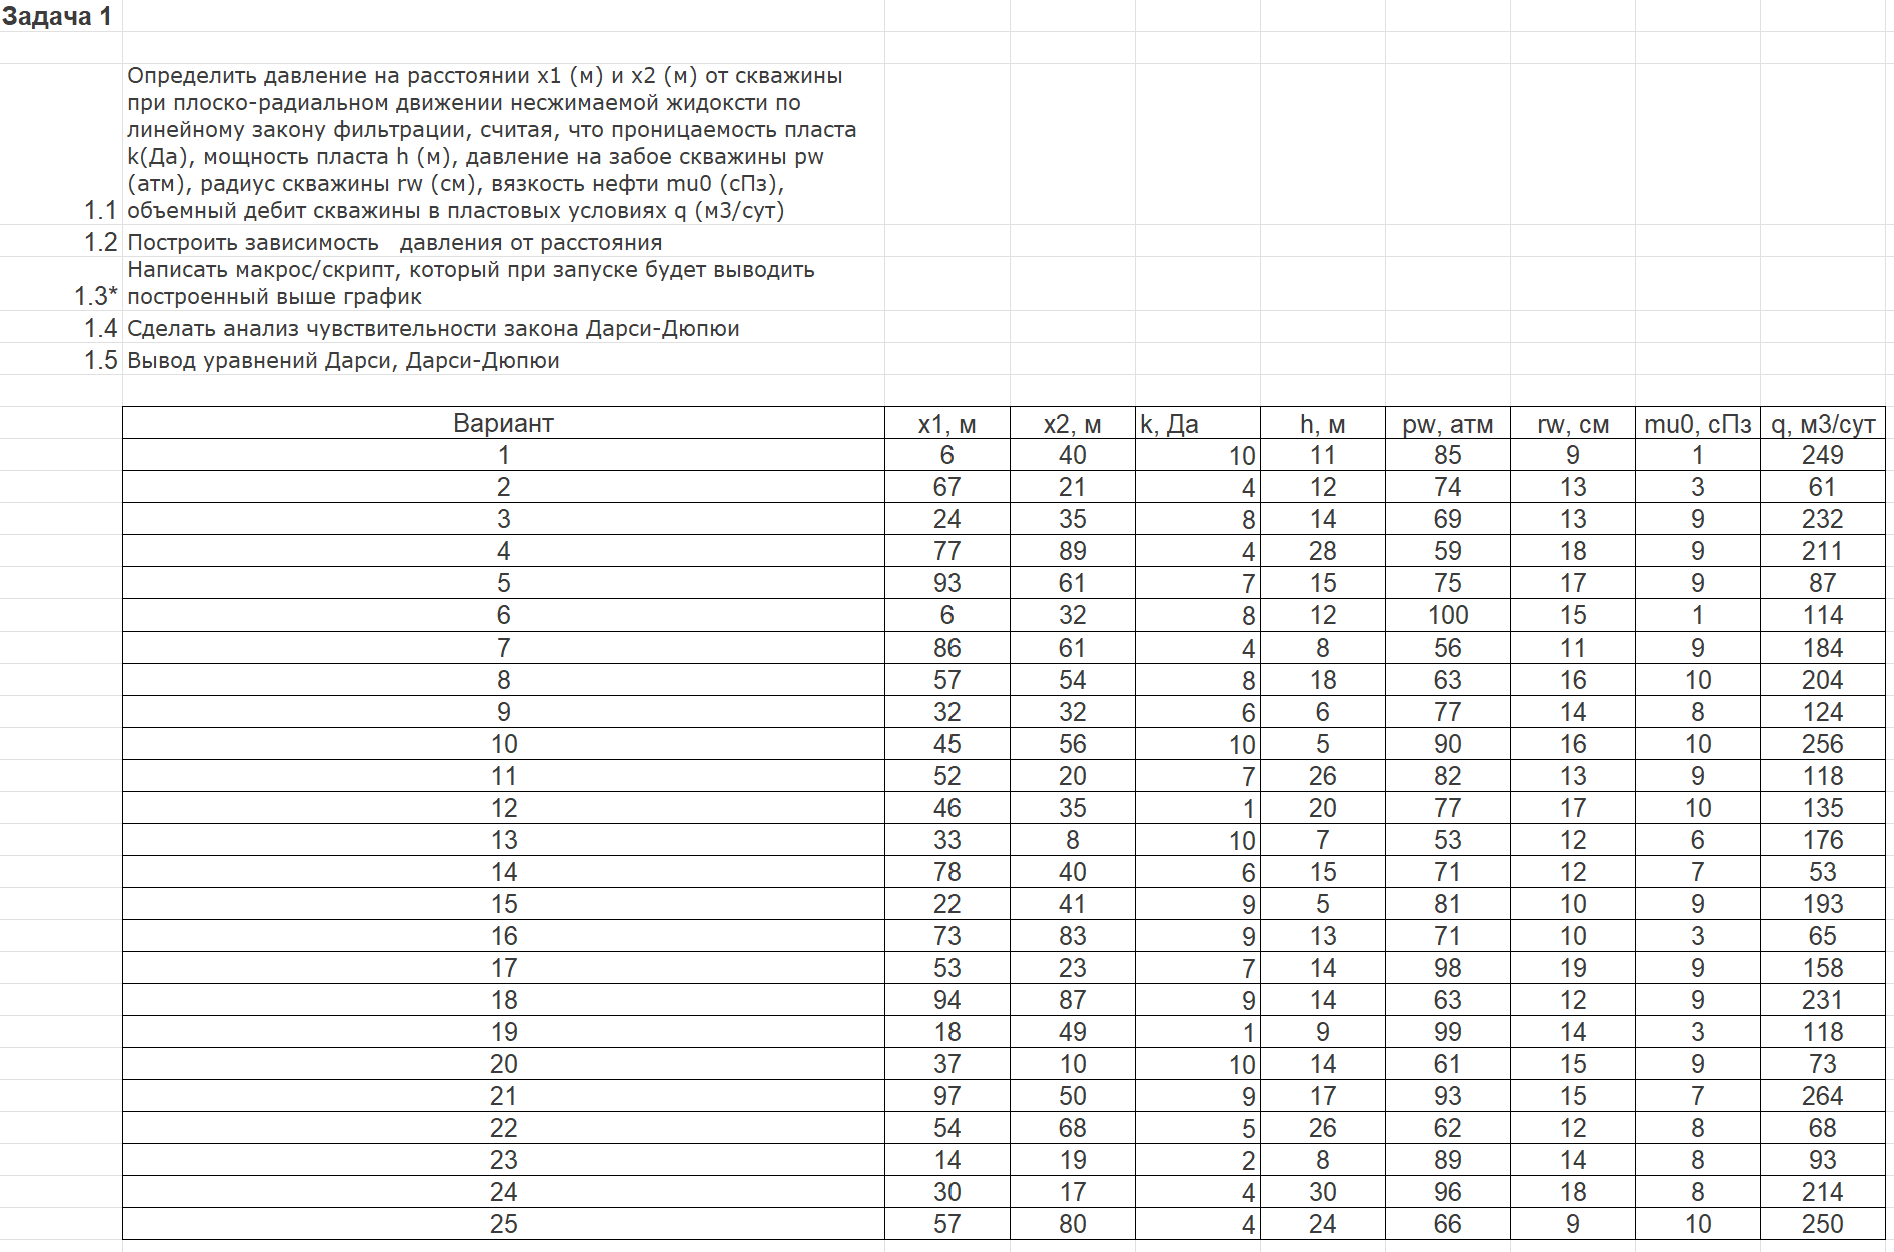
\includegraphics[width=\textwidth]{task1}


\subsection{Расчёт давления по формуле Дюпюи}

Давление на расстоянии $x_1$:
\begin{multline}
P_{x_1}=P_w+\frac{18.41\cdot Q\mu}{kh}\left(\ln{\left(\frac{x_1}{r_w}\right)+S}\right)
=\\=71\text{ атм}+\frac{18.41\cdot 65\dfrac{\text{м}^3}{\text{сут}}\cdot3\text{ сПз}}{9000\text{ мД}\cdot 13\text{ м}}\left(\ln{\left(\frac{73\text{ м}}{0.1\text{ м}}\right)}+0\right)\approx 71.2023\text{ атм}
\end{multline}

Давление на расстоянии $x_2$:
\begin{multline}
P_{x_1}=P_w+\frac{18.41\cdot Q\mu}{kh}\left(\ln{\left(\frac{x_2}{r_w}\right)+S}\right)
=\\=71\text{ атм}+\frac{18.41\cdot 65\dfrac{\text{м}^3}{\text{сут}}\cdot3\text{ сПз}}{9000\text{ мД}\cdot 13\text{ м}}\left(\ln{\left(\frac{83\text{ м}}{0.1\text{ м}}\right)}+0\right)\approx 71.2062\text{ атм}
\end{multline}


\subsection{График зависимости давления от расстояния}

\subsection{Код для вывода графика}

\subsection{Анализ чувствительности формулы Дюпюи}

Вид формулы Дюпюи на установившемся режиме в промысловых единицах со скин-фактором:

\beq
Q=\frac{kh}{18.41\cdot\mu}\,\frac{P_e-P_w}{\ln{\left(\dfrac{r_e}{r_w}\right)+S}}
\eeq

Jupyter-тетрадь с кодом для построения графика и проведения анализа чувствительности доступна по ссылке: \href{https://colab.research.google.com/github/mualal/notebooks-source/blob/master/6_pressure.ipynb}{OPEN IN COLAB}.

\subsection{Вывод уравнения Дарси и формулы Дюпюи}

Приравнивая значение потоковой скорости, найденное из геометрии пласта, к значению, найденному из закона Дарси, получим дифференциальное уравнение притока флюида к скважине.

Дюпюи составил и решил это дифференциальное уравнение для случая границы в виде цилиндрической области (для радиального режима течения).

\beq
\frac{Q}{A}=\frac{k}{\mu}\frac{dP}{dx}\Rightarrow\frac{Q}{2\pi h}\int\limits_{r_w}^{r_e}{\frac{dr}{r}}=\frac{k}{\mu}\int\limits_{P_w}^{P_e}{dp}\Rightarrow Q=\frac{2\pi kh}{\mu}\frac{P_e-P_w}{\ln{\left(\dfrac{r_e}{r_w}\right)}}
\eeq

Формула получена в СИ.
При пересчёте в промысловые единицы измерения формула Дюпюи примет следующий вид:

\beq
Q=\frac{kh}{18.41\cdot\mu}\,\frac{P_e-P_w}{\ln{\left(\dfrac{r_e}{r_w}\right)}}
\eeq

\section{Задание 2 от 14.09.2022}
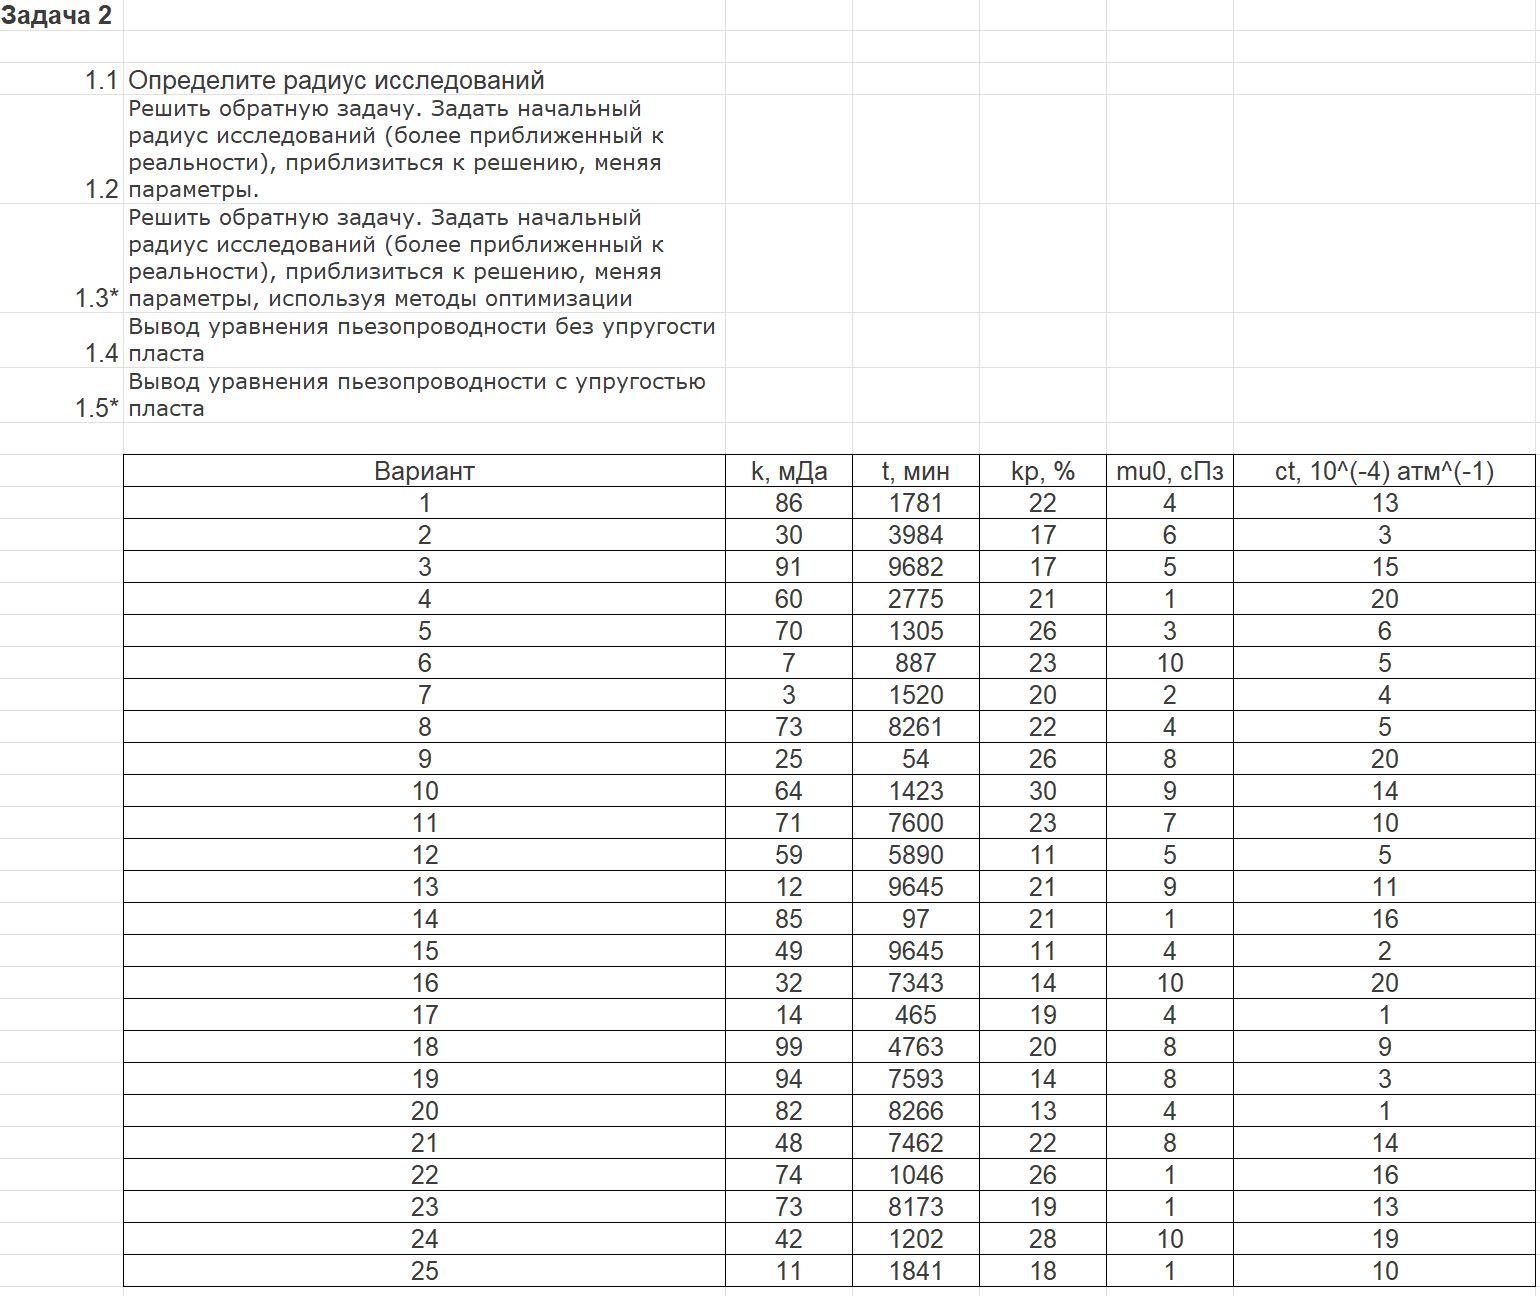
\includegraphics[width=\textwidth]{task2}

\subsection{Радиус исследований}

\beq
r_{inv}=0.037\sqrt{\frac{kt}{\varphi \mu c_t}}=0.037\sqrt{\frac{32\text{ мДа}\cdot 7343\text{ мин}}{0.14\cdot 10\text{ сПз}\cdot 20\cdot 10^{-4}\dfrac{\text{1}}{\text{атм}}}}\approx 338.95\text{ м}
\eeq

График зависимости радиуса исследования от произведения проницаемости и времени построен по ссылке: \href{https://colab.research.google.com/github/mualal/notebooks-source/blob/master/7_exploration_radius.ipynb}{OPEN IN COLAB}.

\subsection{Решение обратной задачи}

Зададим радиус исследования $r_{inv}=100\text{ м}$, тогда:

\beq
kt=\varphi\mu c_t\left(\dfrac{r_{inv}}{0.037}\right)^2=0.14\cdot 10\text{ сПз}\cdot 20\cdot 10^{-4}\frac{1}{\text{атм}}\cdot \left(\frac{100\text{ м}}{0.037}\right)^{\!2}\approx 20452.89\text{ мДа}\cdot\text{мин}
\eeq

При проницаемости $k=32\text{ мДа}$, время исследования будет составлять:

\beq
t\approx\frac{20452.89\text{ мДа}\cdot\text{мин}}{32\text{ мДа}}\approx 639 \text{ мин}\approx10.65\text{ ч}.
\eeq

\subsection{Вывод уравнения пьезопроводности без упругости пласта}

1) Набор уравнений:
\begin{itemize}
	\item неразрывность потока
	\beq\label{Continuity}
	\frac{\partial\left(\rho_f\varphi\right)}{\partial t}+\pmb{\nabla}\cdot\left(\rho_f\varphi \pmb{v_f}\right)=q_f(\pmb{x})
	\eeq
	\item закон Дарси
	\beq\label{Darcy}
	\pmb{W}=-\frac{k}{\mu_f}\cdot\pmb{\nabla} p
	\eeq
	\item сжимаемость флюида
	\beq\label{Compressibility}
	p-p_0=K_f\frac{\rho_f-\rho_f^0}{\rho_f^0}
	\eeq
\end{itemize}

На этих уравнениях строится основное уравнение гидродинамики пласта -- уравнение пьезопроводности.

2) Насыщенности и относительные фазовые проницаемости (для нескольких флюидов)

3) Геометрия (сложное строение пласта)

\subsubsection{В векторной форме (быстрый, но не совсем строгий вывод)}

В предположении неподвижности скелета ($\pmb{v_s}\approx \pmb{0}$ и $\varphi(t)=\textrm{const}$) верно равенство $\pmb{W}\approx\varphi \pmb{v_f}$. Подставляя в закон Дарси \eqref{Darcy}, получаем:
\beq\label{DarcyWithSkeletNotMoving}
\varphi \pmb{v_f}=-\frac{k}{\mu_f}\cdot\pmb{\nabla} p
\eeq

Условие сжимаемости флюида \eqref{Compressibility} перепишем в дифференциальной форме:
\beq\label{CompressibilityDiff}
\frac{\partial p}{\partial t}=\frac{K_f}{\rho_f^0}\frac{\partial\rho_f}{\partial t}
\eeq

Учитывая предположение о неподвижности скелета, перепишем уравнение неразрывности потока:
\beq\label{ContinuityWithSkeletNotMoving}
\varphi\frac{\partial\rho_f}{\partial t}+\pmb{\nabla}\cdot\left(\rho_f\varphi\pmb{v_f}\right)=q_f(\pmb{x})
\eeq

Подставляя \eqref{DarcyWithSkeletNotMoving} и \eqref{CompressibilityDiff} в \eqref{ContinuityWithSkeletNotMoving}, при отсутствии источникового слагаемого ($q_f(\pmb{x})=0$) получаем:
\beq
\varphi\frac{\rho_f^0}{K_f}\frac{\partial p}{\partial t}-\pmb{\nabla}\cdot\left(\rho_f\frac{k}{\mu_f}\pmb{\nabla} p\right)=0
\eeq

При дополнительном условии слабосжимаемости флюида ($\rho_f\approx\rho_f^0=\textrm{const}$) получаем:
\beq
\frac{\partial p}{\partial t}=\frac{kK_f}{\mu_f\varphi}\pmb{\nabla}^2p
\eeq

Это уравнение пьезопроводности (без упругости пласта), полученное в приближении слабосжимаемого флюида, неподвижного и недеформируемого пласта.

\subsubsection{В покомпонентной форме с обезразмериванием (от Шеля Е.В.)}

Запишем ЗСМ для флюида:
\beq
\frac{\partial r_f}{\partial t}+\partial_i\left(r_f v_i^f\right)=0
\eeq

Закон Дарси в "<школьной"> форме:
\beq
Q=-\frac{\Delta p}{L}\frac{k}{\mu}S
\eeq

Закон Дарси в дифференциальной форме:
\beq\label{DarcyDiffShel}
W_i=-\frac{k_{ij}}{\mu}\partial_j p,
\eeq
где $W_i=\varphi v_i^f$ -- потоковая относительная скорость флюида.

Учитывая связь эффективной и истинной плотностей ($r_f=\varphi\rho_f$), перепишем ЗСМ для флюида:
\beq\label{ContinuityShel}
\frac{\partial\left(\rho_f\varphi\right)}{\partial t}+\partial_i\left(\rho_f\varphi v_i^f\right)=0
\eeq

Подставляя \eqref{DarcyDiffShel} в \eqref{ContinuityShel}, получаем:
\beq\label{GeneralPiezo}
\frac{\partial\left(\rho_f\varphi\right)}{\partial t}-\partial_i\left(\rho_f\frac{k_{ij}}{\mu}\partial_j p\right)=0
\eeq

--------------------------------------------------------------------

Замыкающее соотношение (связь плотности флюида и давления):
\beq\label{Zam1}
\rho_f=\rho_f^0\left(1+c_f\left(p-p_0\right)\right),
\eeq
где $c_f$ -- сжимаемость флюида (1/Па).


Замыкающее соотношение (связь пористости и давления):
\beq\label{Zam2}
\varphi=\varphi^0+c_{\text{п}}\left(p-p_0\right),
\eeq
где $c_{\text{п}}$ -- сжимаемость пор (не равно сжимаемости породы).

--------------------------------------------------------------------

Продифференцируем по времени замыкающее соотношение \eqref{Zam1}:
\beq\label{DiffZam1}
\frac{\partial\rho_f}{\partial t}=c_f\rho_f^0\frac{\partial p}{\partial t}
\eeq

Продифференцируем по пространству замыкающее соотношение \eqref{Zam1}:
\beq\label{GradZam1}
\partial_i\rho_f=c_f\rho_f^0\partial_i p
\eeq

Продифференцируем по времени замыкающее соотношение \eqref{Zam2}:
\beq\label{DiffZam2}
\frac{\partial\varphi}{\partial t}=c_\text{п}\frac{\partial p}{\partial t}
\eeq

Продифференцируем по пространству замыкающее соотношение \eqref{Zam2}:
\beq\label{GradZam2}
\partial_i\varphi=c_\text{п}\partial_i p
\eeq

--------------------------------------------------------------------

Раскрывая производные произведений в \eqref{GeneralPiezo}, получаем:
\beq\label{OpenGeneralContinuity}
\frac{\partial\rho_f}{\partial t}\varphi+\rho_f\frac{\partial\varphi}{\partial t}-\frac{k_{ij}}{\mu}\partial_j p\,\partial_i\rho_f-\rho_f\partial_j p\,\partial_i\!\left(\frac{k_{ij}}{\mu}\right)-\rho_f\frac{k_{ij}}{\mu}\left(\partial_i\partial_j p\right)=0
\eeq

Подставляя \eqref{DiffZam1}, \eqref{GradZam1}, \eqref{DiffZam2} и \eqref{GradZam2} в \eqref{OpenGeneralContinuity}, получаем:
\begin{multline}\label{Expanded}
c_f\rho_f^0\frac{\partial p}{\partial t}\varphi+\rho_f c_\text{п}\frac{\partial p}{\partial t}-\frac{k_{ij}}{\mu}\partial_j p\,c_f\rho_f^0\,\partial_i p-\frac{\rho_f}{\mu}\partial_j p\,\partial_i k_{ij}+\\+\rho_f\,\partial_j p\,k_{ij}\frac{\partial\mu}{\partial p}\frac{1}{\mu^2}\partial_i p-\rho_f\frac{k_{ij}}{\mu}\left(\partial_i\partial_j p\right)=0
\end{multline}

--------------------------------------------------------------------

Перед анализом физических уравнений всегда делают масштабный анализ, чтобы понять, какие слагаемые в уравнении важны, а какие не важны (пример: уравнение Навье-Стокса с числами Струхаля, Эйлера, Рейнольдса, Фруда).

Спойлер: ГДМ симуляторы не решают уравнение пьезопроводности в классическом виде, а решают закон сохранения массы, в который они подставляют закон Дарси.

Далее необходимо выделить характерные масштабные факторы, обезразмерив каждую из функций в уравнении.

Введём безразмерное давление $\tilde{p}$ такое, что:
\beq
p=\tilde{p}\cdot p_0,
\eeq
где $p_0$ -- пластовое давление.

Введём безразмерное расстояние $\tilde{r}$ такое, что:
\beq
\vec{r}=\tilde{r}\cdot L,
\eeq
где $L$ -- некое характерное расстояние (например, между скважинами).

Введём безразмерную проницаемость $\tilde{k}_{ij}$ такую, что:
\beq
k_{ij}=\tilde{k}_{ij}\cdot k_0,
\eeq
где $k_0$ -- некая характерная проницаемость.

Введём безразмерную вязкость $\tilde{\mu}$ такую, что:
\beq
\mu=\tilde{\mu}\cdot\mu_0,
\eeq
где $\mu_0$ -- некая характерная вязкость.

Все безразмерные функции (с волной) порядка единицы.

--------------------------------------------------------------------

Перепишем \eqref{Expanded} в введённых безразмерных величинах, разделив обе части этого уравнения на $\rho_f^0$:
\begin{multline}
\frac{\partial p}{\partial t}\left(\varphi c_f+\frac{\rho_f}{\rho_f^0}\cdot c_\text{п}\right)-\frac{k_0}{\mu_0}\frac{p_0^2}{L^2}c_f\frac{\tilde{k}_{ij}}{\tilde{\mu}}\,\tilde{\partial}_i\tilde{p}\,\tilde{\partial}_j\tilde{p}-\frac{\rho_f}{\rho_f^0}\frac{k_0\,p_0}{\mu_0L^2}\frac{\tilde{k}_{ij}}{\tilde{\mu}}\,\tilde{\partial}_j\tilde{p}\,\tilde{\partial}_i\tilde{k}_{ij}+\\+\frac{\rho_f}{\rho_f^0}\frac{p_0\,k_0}{L^2\mu_0}\,\tilde{\partial}_j\tilde{p}\,\tilde{k}_{ij}\frac{\partial\tilde{\mu}}{\partial\tilde{p}}\frac{1}{\tilde{\mu}^2}\,\tilde{\partial}_i\tilde{p}-\frac{\rho_f}{\rho_f^0}\frac{k_0}{\mu_0}\frac{p_0}{L^2}\,\frac{\tilde{k}_{ij}}{\tilde{\mu}}\left(\tilde{\partial}_i\tilde{\partial}_j\tilde{p}\right)=0
\end{multline}

Вынесли все масштабные множители. Далее делим обе части уравнения на множитель перед старшей производной $\left(\text{на }\frac{k_0\,p_0}{\mu_0\,L^2}\right)$, т.е. обезразмериваем уравнение:
\begin{multline}\label{PiezoEqDiv}
\frac{\mu_0L^2}{k_0p_0}\cdot\frac{\partial p}{\partial t}\left(\varphi c_f+\frac{\rho_f}{\rho_f^0}\cdot c_\text{п}\right)-p_0c_f\frac{\tilde{k}_{ij}}{\tilde{\mu}}\,\tilde{\partial}_i\tilde{p}\,\tilde{\partial}_j\tilde{p}-\frac{\rho_f}{\rho_f^0}\frac{\tilde{k}_{ij}}{\tilde{\mu}}\,\tilde{\partial}_j\tilde{p}\,\tilde{\partial}_i\tilde{k}_{ij}+\\+\frac{\rho_f}{\rho_f^0}\frac{\partial\tilde{\mu}}{\partial\tilde{p}}\frac{1}{\tilde{\mu}^2}\tilde{k}_{ij}\,\tilde{\partial}_j\tilde{p}\,\tilde{\partial}_i\tilde{p}-\frac{\rho_f}{\rho_f^0}\frac{\tilde{k}_{ij}}{\tilde{\mu}}\left(\tilde{\partial}_i\tilde{\partial}_j\tilde{p}\right)=0
\end{multline}

--------------------------------------------------------------------

Сделаем 3 важных приближения:
\begin{enumerate}
	\item $p_0 c_f\ll 1$ (прикинем: сжимаемость воды порядка $10^{-5}\text{ атм}^{-1}=10^{-10}\text{ Па}^{-1}$; характерные значения давлений на глубинах, равных нескольким километрам, составляют сотни атмосфер; таким образом, произведение порядка $10^{-3}$, что много меньше единицы; но такое приближение не работает для газа: для него рассматриваемое произведение порядка единицы); это приближение фактически равносильно приближению $\rho_f\approx\rho_f^0$;
	\item $\tilde{\partial}_i\tilde{k}_{ij}\ll 1$ (считаем, что на характерном масштабе задачи по данному направлению проницаемость изменяется незначительно, не больше 10 процентов);
	\item $\dfrac{\partial\tilde{\mu}}{\partial\tilde{p}}\ll 1$ (считаем, что отмасштабированный график проницаемости от давления пологий -- этот факт подтверждается экспериментально -- вязкость слабо зависит от давления)
\end{enumerate}

Тогда уравнение \eqref{PiezoEqDiv} перепишется в следующем виде (убрали слагаемые с пренебрежимо малыми множителями в рамках сделанных приближений и вернулись от безразмерных функций с волной к обычным функциям):
\beq
\frac{\partial p}{\partial t}\underbrace{\left(\varphi c_f+c_\text{п}\right)}_{c_t}-\frac{k_{ij}}{\mu}\partial_i\partial_j p=0
\eeq
(заметим, что если есть анизотропия проницаемости, то лапласиана в уравнении не будет).

Получаем классическое уравнение пьезопроводности:
\beq
\frac{\partial p}{\partial t}-\frac{k_{ij}}{\mu c_t}\partial_i\partial_j p=0,
\eeq
где $c_t$ -- это полная сжимаемость.

Замечание. Но есть литература, в которой $c_t=c_f+\frac{c_\text{п}}{\varphi}$, тогда уравнение пьезопроводности будет выглядеть так:
\beq
\frac{\partial p}{\partial t}-\frac{k_{ij}}{\mu\varphi c_t}\partial_i\partial_j p=0
\eeq

--------------------------------------------------------------------

Пусть тензор проницаемости изотропен $k_{ij}=k_0\cdot\delta_{ij}$, тогда:
\beq
\frac{\partial p}{\partial t}-\frac{k_0}{\mu c_t}\delta_{ij}\,\partial_i\partial_j p=0\Leftrightarrow\frac{\partial p}{\partial t}-\frac{k_0}{\mu c_t}\Delta p=0
\eeq
(получили всем известный вид уравнения пьезопроводности).


\subsection{Вывод уравнения пьезопроводности с упругостью пласта}

Задача со звёздочкой. Ещё думаю.

\section{Задание от 21.09.2022}

\subsection{PVT-свойства нефти}

\subsection{Анизотропия проницаемости}

\subsection{Нормализация относительных фазовых проницаемостей}
Jupyter-тетрадь с кодом обработки ОФП доступна по ссылке: \href{https://github.com/mualal/notebooks-source/blob/master/9_labdata_relative_permeabilities.ipynb}{OPEN IN GITHUB}.


\newpage
\section{Задание от 28.09.2022}

Требуется создать синтетическую BOX-модель. Необходимо:
\begin{itemize}
	\item создать BOX-модель с декартовой сеткой 61*114*40 ячеек с размерами ячеек 100*100*0.2 м, глубина кровли 2000 м, ЗСВ 2008 м;
	\item пористость 0.2, проницаемость по X,Y 100 мД, по Z -- 1 мД;
	\item ОФП и PVT-свойства взять по результатам задания от 21.09.2022;
	\item разместить скважины по 5-точечной схеме (хотя бы один элемент).
\end{itemize}

\subsection{Секция RUNSPEC}
Секция \textbf{RUNSPEC} необходима симулятору для выделения оперативной памяти для хранения данных (значений параметров) модели.
Точное количество памяти требует Eclipse.
В т-Навигаторе память выделяется динамически, поэтому в т-Навигаторе некоторые данные этого раздела игнорируются. 

Зададим название модели, присутствующие в ней фазы (нефть и вода) и метрическую систему единиц.

\begin{eclrun}
NOECHO
RUNSPEC

TITLE
Test_model

OIL
WATER

METRIC
\end{eclrun}

Если хотим только прочитать файл и проверить его на наличие ошибок без запуска расчёта, то используем ключевое слово NOSIM.
Но в данной модели хотим запустить полный расчёт, поэтому закомментируем это ключевое слово.
\begin{eclrun}
-- NOSIM
\end{eclrun}

Зададим количество $Nx$, $Ny$ и $Nz$ ячеек расчётной сетки в направлениях $X$, $Y$, $Z$.

\begin{eclrun}
DIMENS
-- Nx  Ny   Nz
   61  114  40 /
\end{eclrun}

Следующее ключевое слово используется для определения числа областей с различными параметрами моделирования.
Задаваемые числа определяют количество областей с различными свойствами начального равновесия.
В данном примере определим только число регионов (равное 1) с различными начальными данными опции равновесия (эти данные будут задаваться в дальнейшем с помощью ключевого слова EQUIL).
\begin{eclrun}
EQLDIMS
 1  /
\end{eclrun}

Следующее ключевое слово задаёт максимальное число параметров, описывающих аквифер.
Первые 4 по умолчанию; максимальное число водоносных пластов, описанных с помощью аналитической модели, в рассматриваемом примере равно 1; максимальное число блоков сетки, примыкающих к какому-либо водоносному пласту, равно 100000; следующие 2 параметра по умолчанию. Подробнее в руководстве.
\begin{eclrun}
AQUDIMS
  4*  1  100000 /
\end{eclrun}

Укажем, что в модели будет использоваться метод масштабирования конечных точек фазовых проницаемостей и капиллярных давлений.
В параметрах указываются переключатель направленного масштабирования конечных точек (в данном примере NODIR) и переключатель нереверсивного масштабирования конечных точек (в данном примере REVERS).
\begin{eclrun}
ENDSCALE
'NODIR'  'REVERS' /
\end{eclrun}

Следующее ключевое слово задаёт максимальные размерности данных по скважинам.
Всего 12 параметров.
В данном примере зададим только максимальное количество скважин в модели, максимальное количество интервалов перфорации для каждой скважины, максимальное количество групп скважин в модели, максимальное количество скважин в одной группе; остальные параметры оставим по умолчанию равными нулю. 
\begin{eclrun}
WELLDIMS
-- Max_wells  Conn_well  Max_groups  Wells_group
   30         50         2           30   /
\end{eclrun}

Следующее ключевое слово используется для задания числа регионов с различными параметрами моделирования.
В данном примере зададим количество регионов фильтрации, количество регионов с различными PVT-свойствами, макимальное количество различных насыщенностей, задаваемых в одной VPT таблице, максимальное количество различных давлений, задаваемых в одной VPT таблице, количество регионов, для которых необходимо выводить данные о запасах; остальные параметры оставим по умолчанию.
\begin{eclrun}
TABDIMS
--NTSFUN  NTPVT  NSSFUN_nodes  NPPVT_nodes NTFIP
    1      1       30           20         3 /
\end{eclrun}

Следующее ключевое слово используется для задания числа регионов с различными параметрами моделирования.
Задаваемые 4 числа определяют:
количество регионов, для которых необходимо выводить данные о запасах (может быть задано также с помощью TABDIMS);
количество множеств регионов, для которых необходимо выводить данные о запасах;
количество регионов с независимыми месторождениями;
количество регионов потока.

В данном примере зададим только первый параметр (который фактически уже задали в TABDIMS); значения остальных параметров оставим по умолчанию.
\begin{eclrun}
REGDIMS
--fipnum fipxx isolnum fluxnum 
 3  /
\end{eclrun}

Укажем максимальное количество векторов в summary файле.
\begin{eclrun}
SMRYDIMS
1000000  /
\end{eclrun}

Выходные и входные файлы унифицированы.
\begin{eclrun}
UNIFOUT
UNIFIN
\end{eclrun}

Укажем дату начала моделирования.
\begin{eclrun}
START
1 'NOV' 2022 /
\end{eclrun}

Включим возможность использования опций обработки данных сетки
\begin{eclrun}
GRIDOPTS
YES /
\end{eclrun}

Зададим ограничения на печать сообщений разных типов, а также условия на остановку расчёта при большом количестве сообщений.
\begin{eclrun}
MESSAGES
-- print                                            
-- message comment warning problem  error   bug     
   1000000 1000000 1000000 10000000 1000000 1000000
-- stop
-- message comment warning problem error bug
   1000000 1000000 1000000 100000  1000  1000  /
\end{eclrun}

\subsection{Секция GRID}
Секция \textbf{GRID} необходима для задания геометрии и фильтрационно-ёмкостных свойств (ФЕС) модели.

Ключевое слово EQUALS позволяет задать значение любого параметра сетки для ячеек, выбранных в область параллелепипеда.

Зададим размеры ячеек DX, DY, DZ в направлениях X, Y, Z соответственно. По умолчанию размеры задаются для каждой из ячеек сетки. 
При этом симулятор строит блочно-центрированную геометрию сетки.
В дальнейшем (уже за рамками данного примера) будем использовать и геометрию угловой точки (с помощью ключевых слов COORD и ZCORN).
\begin{eclrun}
GRID

EQUALS
'DX'    100  /
'DY'    100  /
'DZ'    0.2  /
/
\end{eclrun}


Далее зададим глубину залегания верхнего слоя ячеек.
После значения 2000 заданы 4 параметра по умолчанию (начало интервала по X, конец интервала по X, начало интервала по Y, конец интервала по Y -- по умолчанию заданы все ячейки в направлениях X и Y) и два параметра (начало интервала по Z, конец интервала по Z) равны 1 (т.е. задаём ячейки только верхнего слоя).
Таким образом, значение TOPS 2000 применяется только к ячейкам верхнего слоя. Для других слоёв симулятор автоматически определяет значение, основываясь на высоте ячеек. 
\begin{eclrun}
EQUALS
'TOPS' 2000 4* 1 1 /
/
\end{eclrun}

Далее определяем, что все ячейки модели активны, и задаём пористость и проницаемость по X, Y, Z во всех ячейках.
\begin{eclrun}
EQUALS
'ACTNUM'  1  /
'PORO'  0.2  /
'PERMX' 100  /
'PERMY' 100  /
'PERMZ'  1  /
/
\end{eclrun}

Скажем симулятору, что необходимо записать исходные данные со свойствами сетки и таблицами насыщенностей в файл, который в дальнейшем можно будет прочесть в графических пакетах.
\begin{eclrun}
INIT
\end{eclrun}

\subsection{Секция EDIT}

Опциональная секция с возможностью редактирования данных \textbf{GRID} секции.
В данном примере оставим эту секцию пустой.
\begin{eclrun}
EDIT
\end{eclrun}

\subsection{Секция PROPS}

Секция \textbf{PROPS} необходима для задания параметров флюидов, относительных фазовых проницаемостей и распределения жидкостей на основе функций капиллярных давлений.

Определим PVT-свойства воды.
Задаются опорное давление, коэффициент объёмного расширения воды, коэффициент сжимаемости воды, вязкость воды и производная вязкости воды по давлению.
\begin{eclrun}
PROPS

PVTW          
--P    Bw      cw        muw     dmuw/dpres  
159.6  1.0264  4.32E-05  0.3253  0  /
\end{eclrun}

Определим упругие свойства породы.
Задаются опорное давление, сжимаемость породы, сжимаемость скелета породы, сжимаемость блока (блока, содержащего смесь), значение пористости при опорном давлении, значение коэффициента Пуассона при опорном давлении.
В данном примере укажем значения только для опорного давления и сжимаемости породы; остальные параметры оставим по умолчанию (см. руководство).
\begin{eclrun}
ROCK
--Pref  Compr 
159.6  4.765E-05  /
\end{eclrun}

Зададим плотности нефти и воды в поверхностных условиях.
\begin{eclrun}
DENSITY 
860  1007.5  /
\end{eclrun}

Следующее ключевое слово служит для задания постоянной и однородной концентрации растворённого газа в нефти.
Это обеспечивает наиболее эффективное моделирование системы чёрная нефть, где нет отдельной газовой фазы и давление никогда не опускается ниже точки давления насыщения.

Указаны концентрация растворённого газа и давление насыщения (расчёт будет завершён, если давление в каком-либо блоке сетки опустится ниже этого значения).
\begin{eclrun}
RSCONST 
--Rs  Pb
  20  34  /
\end{eclrun}


Следующее ключевое слово используется для задания PVT-свойств нелетучей нефти для рассматриваемых PVT-регионов.

Необходимо ввести следующие параметры: давление насыщения, коэффициент объёмного расширения нефти, вязкость нефти при давлении насыщения.

PVT свойства нелетучей нефти для каждого PVT региона вводятся в таблицы.
Количество таблиц равно количеству регионов, определённых в TABDIMS.

В рассматриваемом примере одна таблица для единственного региона.
Таблица получена в Excel-файле при выполнении задания от 21.09.2022.

\begin{eclrun}
PVDO 
--P     Bo      muo
34     1.06000  9.00000
40     1.05926  9.08157
60     1.05681  9.35346
80     1.05436  9.62535
100    1.05192  9.89724
120    1.04948  10.16913
140    1.04705  10.44102
159.6  1.04467  10.70748
180    1.04220  10.98481
200    1.03978  11.25670
220    1.03737  11.52859
240    1.03497  11.80048
260    1.03257  12.07237
280    1.03018  12.34427
300    1.02779  12.61616
/
\end{eclrun}

Следующее ключевое слово можно указывать, если в секции \textbf{RUNSPEC} присутствует ключевое слово ENDSCALE.
Позволяет задать трёхточечный метод масштабирования конечных точек фазовых проницаемостей.
Указывается один аргумент, имеющий 2 возможных значения (YES -- да, трёхточечный метод масштабирования, NO -- нет, 2-точечный метод)
\begin{eclrun}
SCALECRS
YES /
\end{eclrun}


Зададим таблицы нормализованных относительных фазовых проницаемостей для систем вода-нефть для каждого региона фильтрации (количество регионов задано в TABDIMS -- в рассматриваемом примере один единственный регион -- следовательно, только одна таблица).

Таблица содержит 4 колонки со следующими параметрами: водонасыщенность (SW), проницаемость воды (KRWO), проницаемость нефти (KROW), капиллярное давление фазы нефть-вода (POW).
\begin{eclrun}
SWOF
--Sw     Krw     Kro     Pc
0.0  0.000000  1.000000  0.22100
0.1  0.049403  0.675833  0.11707
0.2  0.122172  0.436130  0.04704
0.3  0.207486  0.265435  0.02680
0.4  0.302128  0.149624  0.01752
0.5  0.404371  0.075953  0.01231
0.6  0.513110  0.033125  0.00900
0.7  0.627566  0.011364  0.00673
0.8  0.747156  0.002516  0.00507
0.9  0.871424  0.000191  0.00333
1.0  1.000000  0.000000  0.00000
/
\end{eclrun}

С помощью следующего ключевого слова задаём арифметические и алгебраические операции над параметрами сетки для ячеек, выбранных в область параллелепипеда.
Задаваемые значения: изменяемый параметр сетки; изменяемая область параллелепипеда; операция; параметр сетки, являющийся аргументом; скалярный параметр 1, если нужен; скалярный параметр 2, если нужен.

В рассматриваемом примере задаём корреляции остаточных насыщенностей и концевых точек от ФЕС ячейки.
Коэффициенты корреляций (скалярные параметры) найдены при выполнении задания от 21.09.2022.

Остаточные насыщенности и концевые точки необходимы для проведения масштабирования ранее заданных нормализованных ОФП.
\begin{eclrun}
OPERATE
SWCR   1 61  1 114  1 40  'LOGE'   PERMX /
SWCR   1 61  1 114  1 40  'MULTA'  SWCR  -0.04705  0.52721  /
SOWCR  1 61  1 114  1 40  'LOGE'   PERMX /
SOWCR  1 61  1 114  1 40  'MULTA'  SOWCR  -0.01289  0.27396 /
KRWR   1 61  1 114  1 40  'LOGE'   PERMX /
KRWR   1 61  1 114  1 40  'MULTA'  KRWR   0.06701  -0.14287 /
--Krw@(Sw=1-Sowcr)
/
\end{eclrun}

Далее для всех ячеек задаём:
максимальную водонасыщенность;
относительная проницаемость по нефти при критической водонасыщенности;
максимальное значение относительной проницаемости по нефти;
максимальное значение относительной проницаемости по воде
(все задаваемые значения используются при масштабировании конечных точек насыщенностей).
\begin{eclrun}
EQUALS
SWU 1 /--MAX Sw
KRORW  0.833 /--Kro@(Sw=Swcr)
KRO 1 /-- Kro@(SW=0)
KRW 1 /-- Krw@(SW=1)
/
\end{eclrun}

Далее зададим минимальную водонасыщенность ячеек SWL, используемую при масштабировании конечных точек насыщенностей (скопируем значения из критических водонасыщенностей SWCR).
\begin{eclrun}
COPY
SWCR SWL /--MIN Sw
/
\end{eclrun}


\subsection{Секция REGION}

Секция \textbf{REGION} позволяет определить регионы (области) модели с разными свойствами.
В данном примере оставим эту секцию пустой.
\begin{eclrun}
REGIONS
\end{eclrun}


\subsection{Секция SOLUTION}

В секции \textbf{SOLUTION} доопределяются параметры, необходимые для инициализации модели.

Следующее ключевое слово задаёт для каждого региона равновесия (в рассматриваемом примере один единственный регион) свойства, используемые при расчёте начальных условий.
Рассматривается равновесный способ инициализации.

Указаны: глубина; давление на этой глубине; глубина водо-нефтяного контакта; капиллярное давление на глубине водо-нефтяного контакта (если 0, то это зеркало свободной воды); глубина газо-нефтяного контакта; капиллярное давление на глубине газо-нефтяного контакта; далее см. руководство.

\begin{eclrun}
SOLUTION

EQUIL
--FWLs
2008   200.8   2008   0   1000   0  1  0  1*  /
\end{eclrun}

Следующее ключевое слово осуществляет управление выходными данными секции \textbf{SOLUTION}.
\begin{eclrun}
RPTSOL
'FIP=2' 'SWATINIT' /
\end{eclrun}

\subsection{Секция SUMMARY}

В секции \textbf{SUMMARY} определяются векторы, которые запишутся в файлы с результатом расчёта, и их формат.

\begin{eclrun}
SUMMARY

ALL
SEPARATE
EXCEL
RUNSUM
RPTONLY
\end{eclrun}

\subsection{Секция SCHEDULE}

В секции \textbf{SCHEDULE} определяются скважины, группы скважин, график работы, требования к отчётности и т.п.

Следующее ключевое слово осуществляет контроль вывода данных в restart файл.
\begin{eclrun}
SCHEDULE

RPTRST
--report every timestep
'BASIC=2' 'FREQ=1'  /
\end{eclrun}


Зададим структуру иерархии групп скважин.
\begin{eclrun}
GRUPTREE
'INJECT'  'FIELD'  /
'PRODUCE' 'FIELD'  /
/
\end{eclrun}

Следующее ключевое слово определяет информацию о забое скважин.

Вводятся следующие данные для каждой из скважин:
название скважины;
название группы скважин, к которой принадлежит данная скважина;
координата ячейки по оси X, в которой расположен забой или устье скважины;
координата ячейки по оси Y, в которой расположен забой или устье скважины;
опорная глубина для забойного давления (по умолчанию глубина первого интервала перфорации);
предпочтительная фаза для скважины (данные этого параметра используются для определения индекса продуктивности/приёмистости скважины, или её потенциального расхода);
далее см. руководство.

\begin{eclrun}
WELSPECS
-- name   group      iw  jw ref.depth phase
'INJ1'    'INJECT'   30  75  1*  'WATER'  /
'INJ2'    'INJECT'   40  75  1*  'WATER'  /
'INJ3'    'INJECT'   20  75  1*  'WATER'  /
'INJ4'    'INJECT'   20  65  1*  'WATER'  /
'INJ5'    'INJECT'   30  65  1*  'WATER'  /
'INJ6'    'INJECT'   40  65  1*  'WATER'  /
'INJ7'    'INJECT'   20  55  1*  'WATER'  /
'INJ8'    'INJECT'   30  55  1*  'WATER'  /
'INJ9'    'INJECT'   40  55  1*  'WATER'  /
'PR_01'  'PRODUCE'   25  70  1*    'OIL'  /
'PR_02'  'PRODUCE'   25  80  1*    'OIL'  /
'PR_03'  'PRODUCE'   35  70  1*    'OIL'  /
'PR_04'  'PRODUCE'   35  80  1*    'OIL'  /
'PR_05'  'PRODUCE'   45  80  1*    'OIL'  /
'PR_06'  'PRODUCE'   45  70  1*    'OIL'  /
'PR_07'  'PRODUCE'   15  80  1*    'OIL'  /
'PR_08'  'PRODUCE'   15  70  1*    'OIL'  /
'PR_09'  'PRODUCE'   15  60  1*    'OIL'  /
'PR_10'  'PRODUCE'   25  60  1*    'OIL'  /
'PR_11'  'PRODUCE'   35  60  1*    'OIL'  /
'PR_12'  'PRODUCE'   45  60  1*    'OIL'  /
'PR_13'  'PRODUCE'   15  50  1*    'OIL'  /
'PR_14'  'PRODUCE'   25  50  1*    'OIL'  /
'PR_15'  'PRODUCE'   35  50  1*    'OIL'  /
'PR_16'  'PRODUCE'   45  50  1*    'OIL'  /
/
\end{eclrun}

Следующее ключевое слово определяет интервалы перфорации скважины и траекторию скважины.

Вводятся следующие данные:
название скважины (или номер);
координата участка перфорации по оси X;
координата участка перфорации по оси Y;
слой, с которого начинается вертикальный участок перфорации скважины;
слой, на котором заканчивается вертикальный участок перфорации скважины;
состояние перфорации;
номер таблицы фильтрации;
коэффициент проводимости для каждого блока в интервале перфорации;
диаметр скважины;
гидропроводность (КН) для каждого блока в интервале перфорации;
скин $S$;
D-фактор скважины для течения не-Дарси;
пространственная ориентация скважины (X, Y или Z);
эффективный радиус $r_o$.

\begin{eclrun}
COMPDAT
'INJ1'   30  75  1 40 'OPEN' 2* 0.16  1* 0 1* 'Z' 1* /
'INJ2'   40  75  1 40 'OPEN' 2* 0.16  1* 0 1* 'Z' 1* /
'INJ3'   20  75  1 40 'OPEN' 2* 0.16  1* 0 1* 'Z' 1* /
'INJ4'   20  65  1 40 'OPEN' 2* 0.16  1* 0 1* 'Z' 1* /
'INJ5'   30  65  1 40 'OPEN' 2* 0.16  1* 0 1* 'Z' 1* /
'INJ6'   40  65  1 40 'OPEN' 2* 0.16  1* 0 1* 'Z' 1* /
'INJ7'   20  55  1 40 'OPEN' 2* 0.16  1* 0 1* 'Z' 1* /
'INJ8'   30  55  1 40 'OPEN' 2* 0.16  1* 0 1* 'Z' 1* /
'INJ9'   40  55  1 40 'OPEN' 2* 0.16  1* 0 1* 'Z' 1* /
'PR_01'  25  70  1 20 'OPEN' 2* 0.16  1* 0 1* 'Z' 1* /
'PR_02'  25  80  1 20 'OPEN' 2* 0.16  1* 0 1* 'Z' 1* /
'PR_03'  35  70  1 20 'OPEN' 2* 0.16  1* 0 1* 'Z' 1* /
'PR_04'  35  80  1 20 'OPEN' 2* 0.16  1* 0 1* 'Z' 1* /
'PR_05'  45  80  1 20 'OPEN' 2* 0.16  1* 0 1* 'Z' 1* /
'PR_06'  45  70  1 20 'OPEN' 2* 0.16  1* 0 1* 'Z' 1* /
'PR_07'  15  80  1 20 'OPEN' 2* 0.16  1* 0 1* 'Z' 1* /
'PR_08'  15  70  1 20 'OPEN' 2* 0.16  1* 0 1* 'Z' 1* /
'PR_09'  15  60  1 20 'OPEN' 2* 0.16  1* 0 1* 'Z' 1* /
'PR_10'  25  60  1 20 'OPEN' 2* 0.16  1* 0 1* 'Z' 1* /
'PR_11'  35  60  1 20 'OPEN' 2* 0.16  1* 0 1* 'Z' 1* /
'PR_12'  45  60  1 20 'OPEN' 2* 0.16  1* 0 1* 'Z' 1* /
'PR_13'  15  50  1 20 'OPEN' 2* 0.16  1* 0 1* 'Z' 1* /
'PR_14'  25  50  1 20 'OPEN' 2* 0.16  1* 0 1* 'Z' 1* /
'PR_15'  35  50  1 20 'OPEN' 2* 0.16  1* 0 1* 'Z' 1* /
'PR_16'  45  50  1 20 'OPEN' 2* 0.16  1* 0 1* 'Z' 1* /
/
\end{eclrun}


Следующее ключевое слово управляет нагнетательными скважинами.

Вводятся следующие данные:
название скважины (или номер) или список скважин;
тип закачиваемого флюида;
режим работы скважины (открыта, остановлена или закрыта);
управление скважиной (контроль по объёму закачки RATE, контроль по забойному давлению BHP и т.д.);
объём закачки для нагнетательной скважины в поверхностных условиях;
объём закачки для нагнетательной скважины в пластовых условиях;
забойное давление или ограничение по забойному давлению;
далее см. руководство. 

\begin{eclrun}
WCONINJE
 'INJ1' 'WATER' 'OPEN' 'BHP' 2* 450 /
 'INJ2' 'WATER' 'OPEN' 'BHP' 2* 450 /
 'INJ3' 'WATER' 'OPEN' 'BHP' 2* 450 /
 'INJ4' 'WATER' 'OPEN' 'BHP' 2* 450 /
 'INJ5' 'WATER' 'OPEN' 'BHP' 2* 450 /
 'INJ6' 'WATER' 'OPEN' 'BHP' 2* 450 /
 'INJ7' 'WATER' 'OPEN' 'BHP' 2* 450 /
 'INJ8' 'WATER' 'OPEN' 'BHP' 2* 450 /
 'INJ9' 'WATER' 'OPEN' 'BHP' 2* 450 /
/
\end{eclrun}


Следующее ключевое слово управляет добывающими скважинами.

Вводятся следующие данные:
название скважины (или номер) или список скважин;
режим работы скважины (открыта, остановлена или закрыта);
управление скважиной (контроль по дебиту жидкости LRAT, контроль по забойному давлению BHP и т.д.);
дебит нефти в поверхностных условиях (или ограничение по дебиту нефти);
дебит воды в поверхностных условиях (или ограничение по дебиту воды);
дебит газа в поверхностных условиях (или ограничение по дебиту газа);
дебит жидкости на поверхности (или ограничение по дебиту жидкости);
дебит жидкости в пласте (или ограничение по дебиту жидкости в пласте);
величина забойного давления или ограничение по забойному давлению;
далее см. руководство. 

\begin{eclrun}
WCONPROD
 'PR_01' 'OPEN' 'BHP' 5* 50 /
 'PR_02' 'OPEN' 'BHP' 5* 50 /
 'PR_03' 'OPEN' 'BHP' 5* 50 /
 'PR_04' 'OPEN' 'BHP' 5* 50 /
 'PR_05' 'OPEN' 'BHP' 5* 50 /
 'PR_06' 'OPEN' 'BHP' 5* 50 /
 'PR_07' 'OPEN' 'BHP' 5* 50 /
 'PR_08' 'OPEN' 'BHP' 5* 50 /
 'PR_09' 'OPEN' 'BHP' 5* 50 /
 'PR_10' 'OPEN' 'BHP' 5* 50 /
 'PR_11' 'OPEN' 'BHP' 5* 50 /
 'PR_12' 'OPEN' 'BHP' 5* 50 /
 'PR_13' 'OPEN' 'BHP' 5* 50 /
 'PR_14' 'OPEN' 'BHP' 5* 50 /
 'PR_15' 'OPEN' 'BHP' 5* 50 /
 'PR_16' 'OPEN' 'BHP' 5* 50 /
/
\end{eclrun}

Определим длину (в днях) и количество временных шагов моделирования.
\begin{eclrun}
TSTEP
48*30 /
\end{eclrun}

Завершим чтение файла.
\begin{eclrun}
END
\end{eclrun}


Далее приведены несколько результатов расчёта построенной box-модели.

\begin{figure}[H]
\center
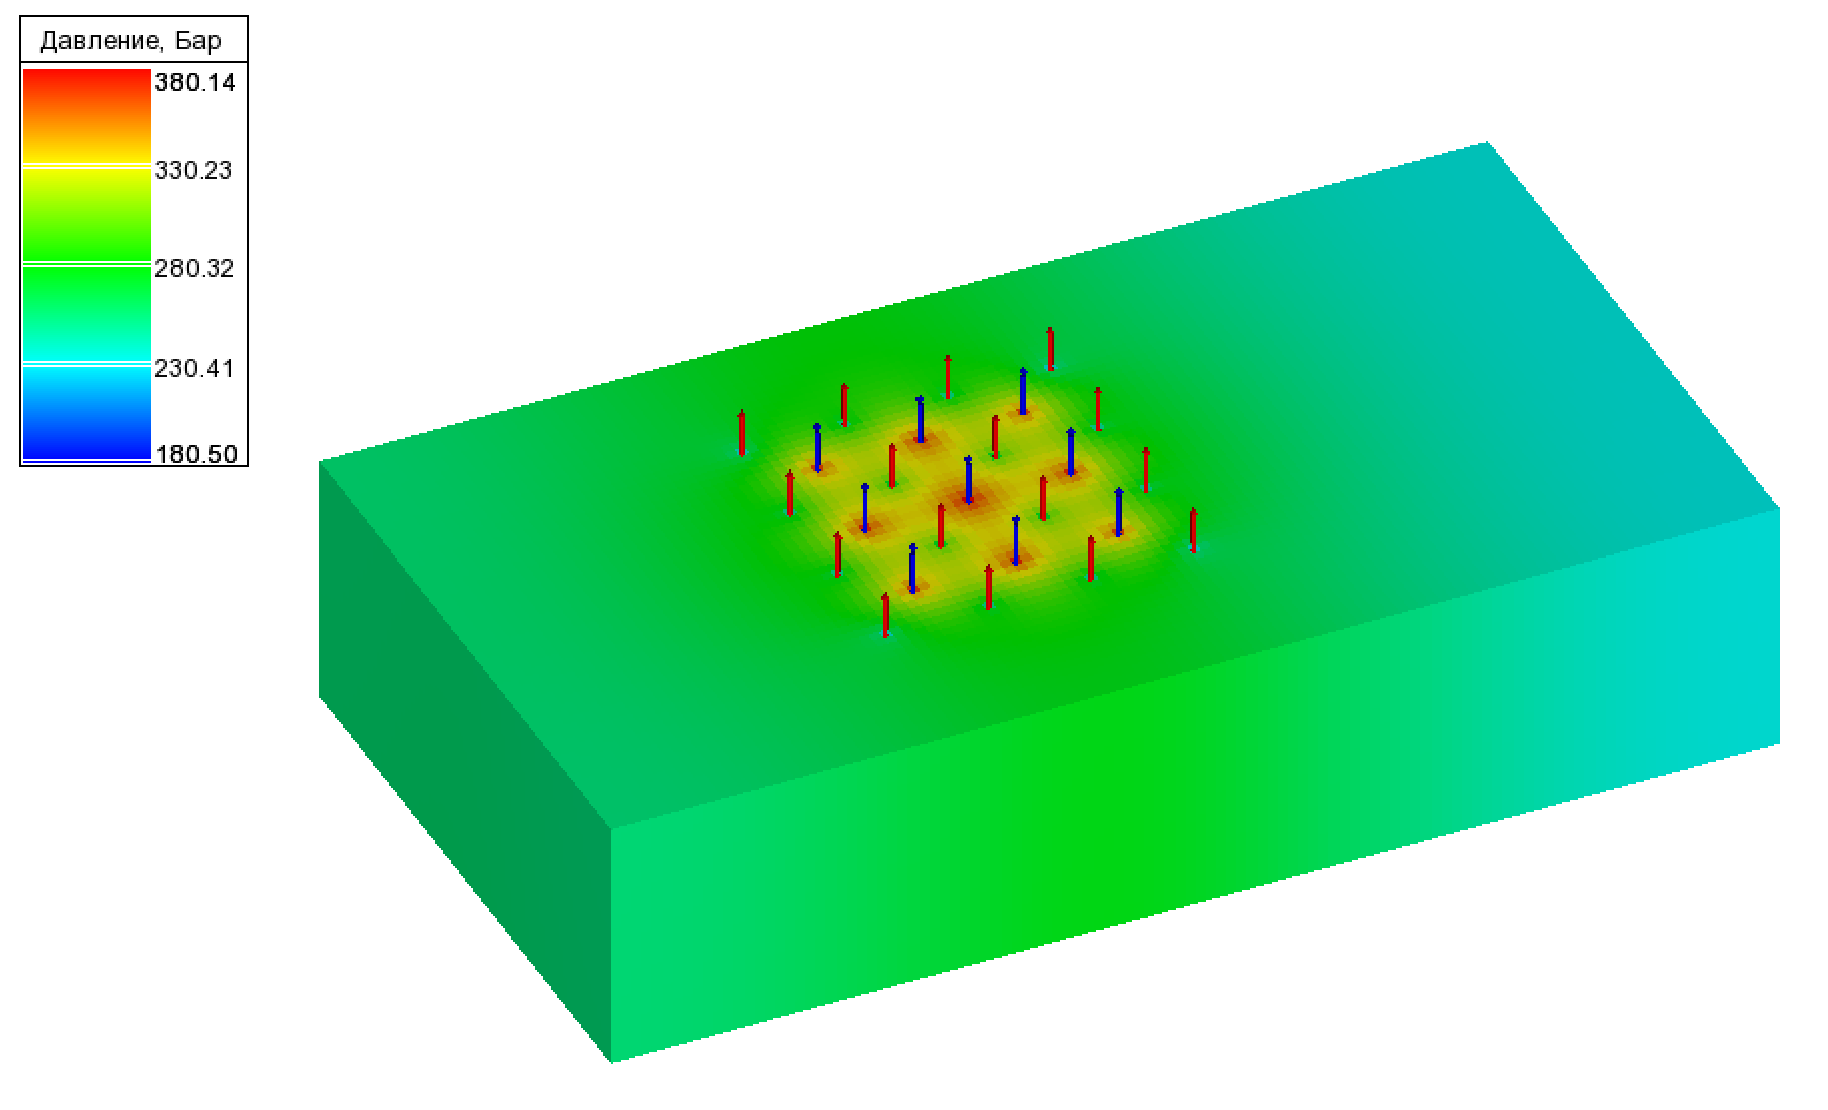
\includegraphics[width=\textwidth]{tnav_pressure_box_model}
\caption{Распределение давлений в последний месяц моделирования -- визуализация tNavigator}
\label{fig:tnav_pressure_box_model}
\end{figure}

\begin{figure}[H]
\center
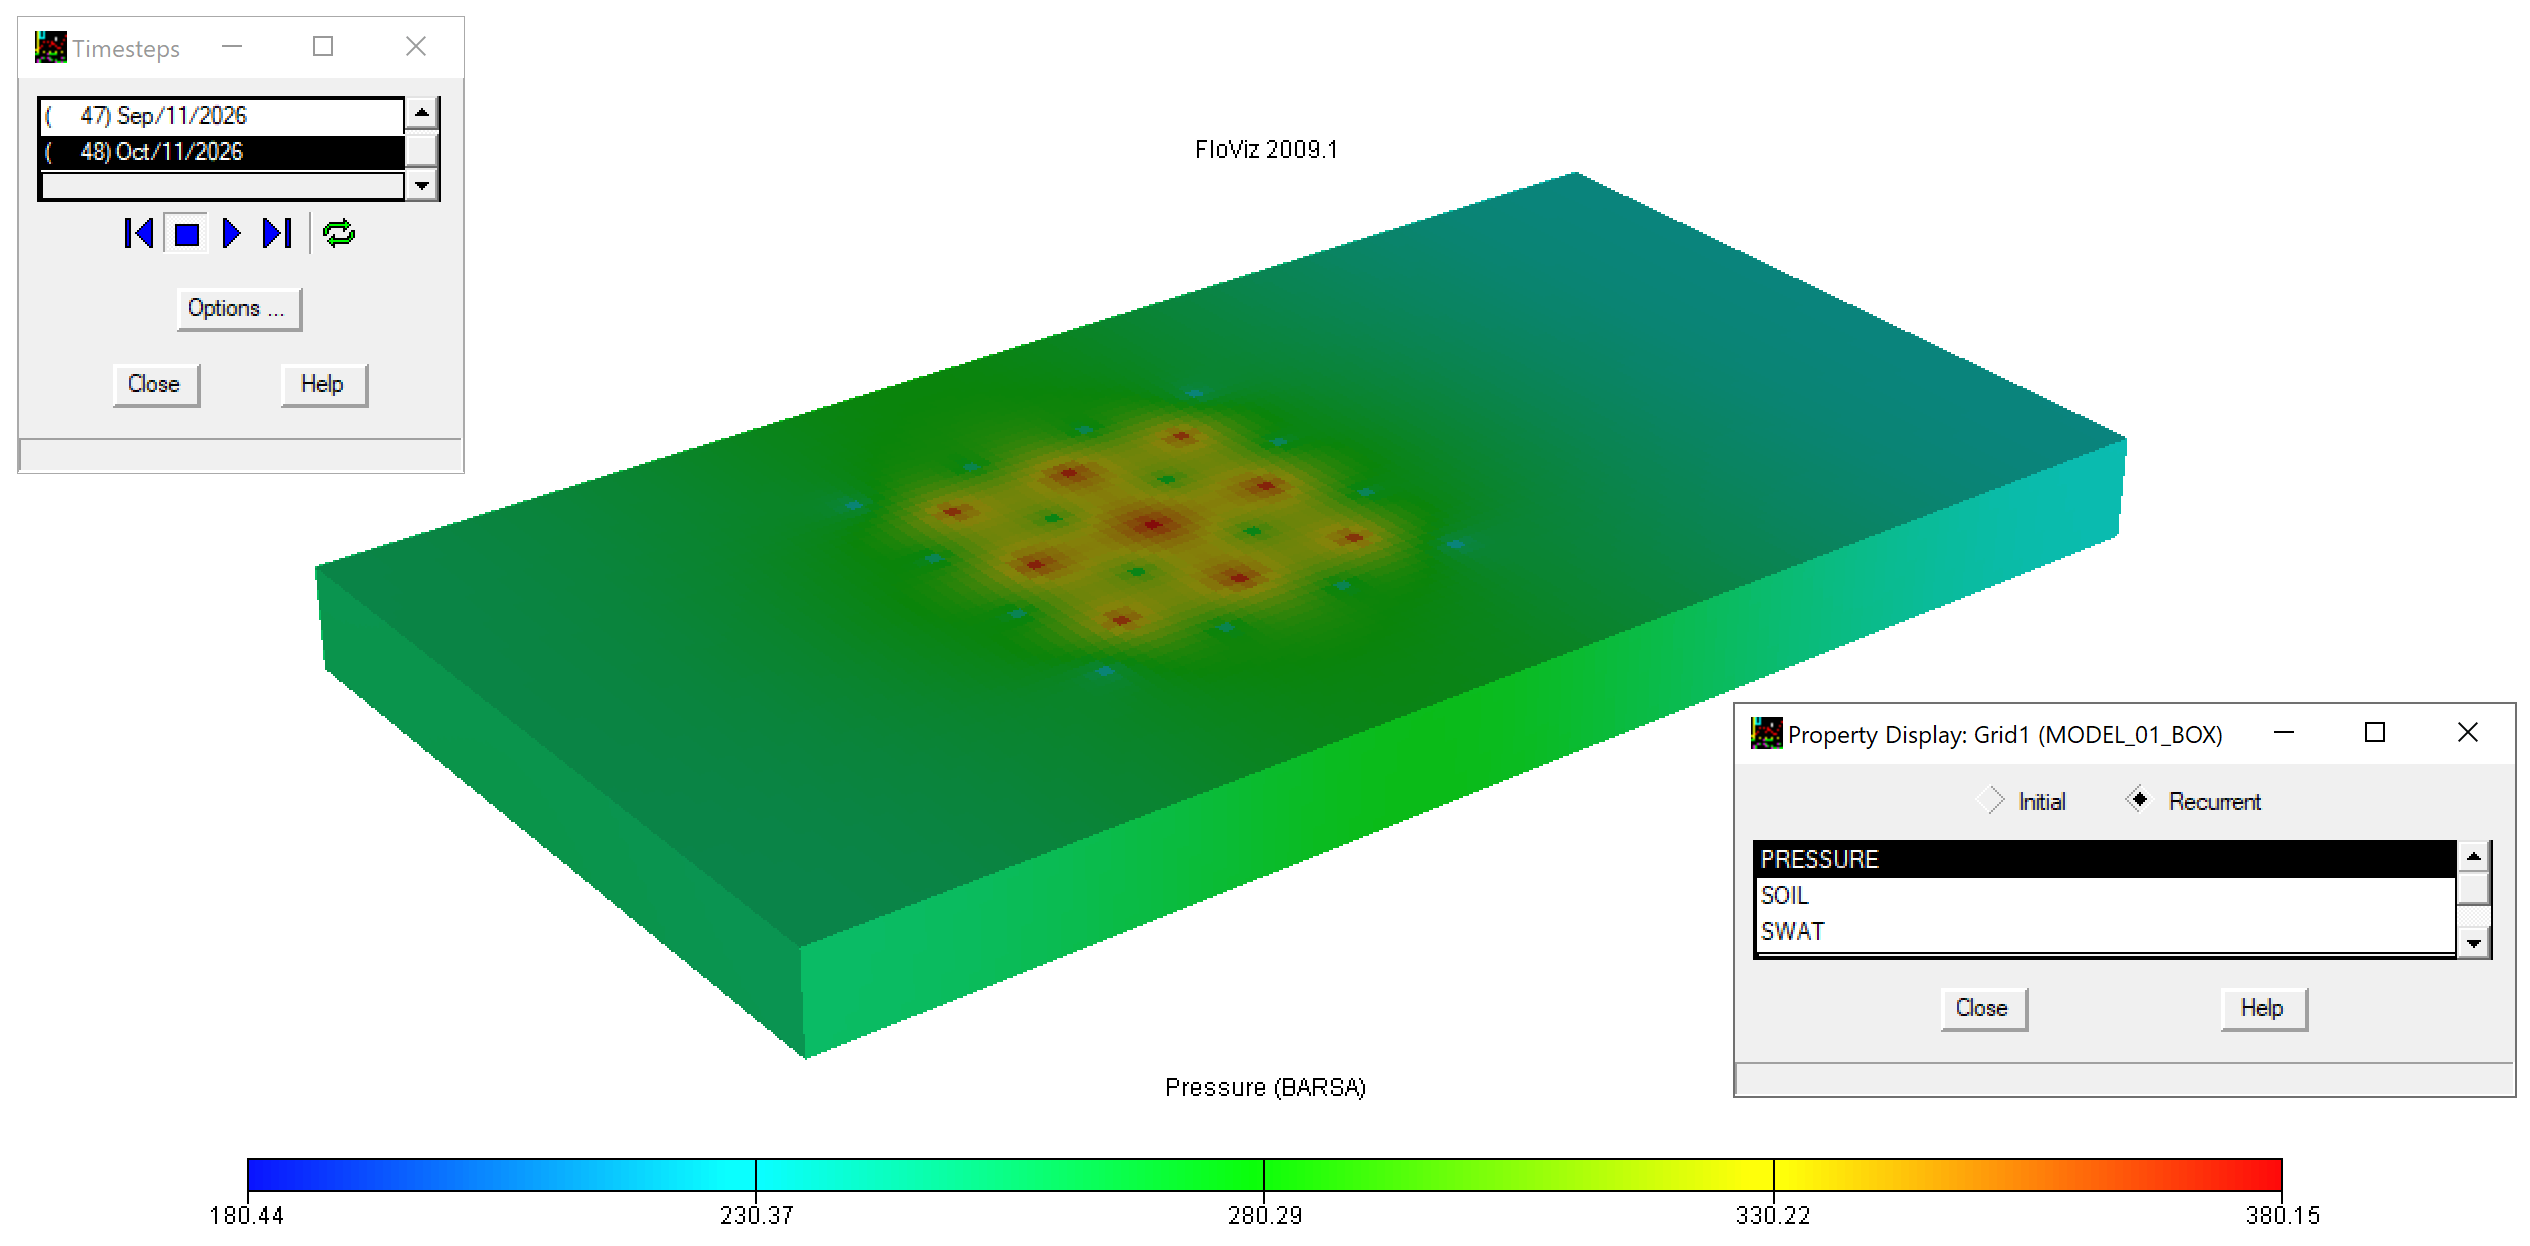
\includegraphics[width=\textwidth]{ecl_pressure_box_model}
\caption{Распределение давлений в последний месяц моделирования -- визуализация FloViz}
\label{fig:ecl_pressure_box_model}
\end{figure}


\begin{figure}[H]
\center
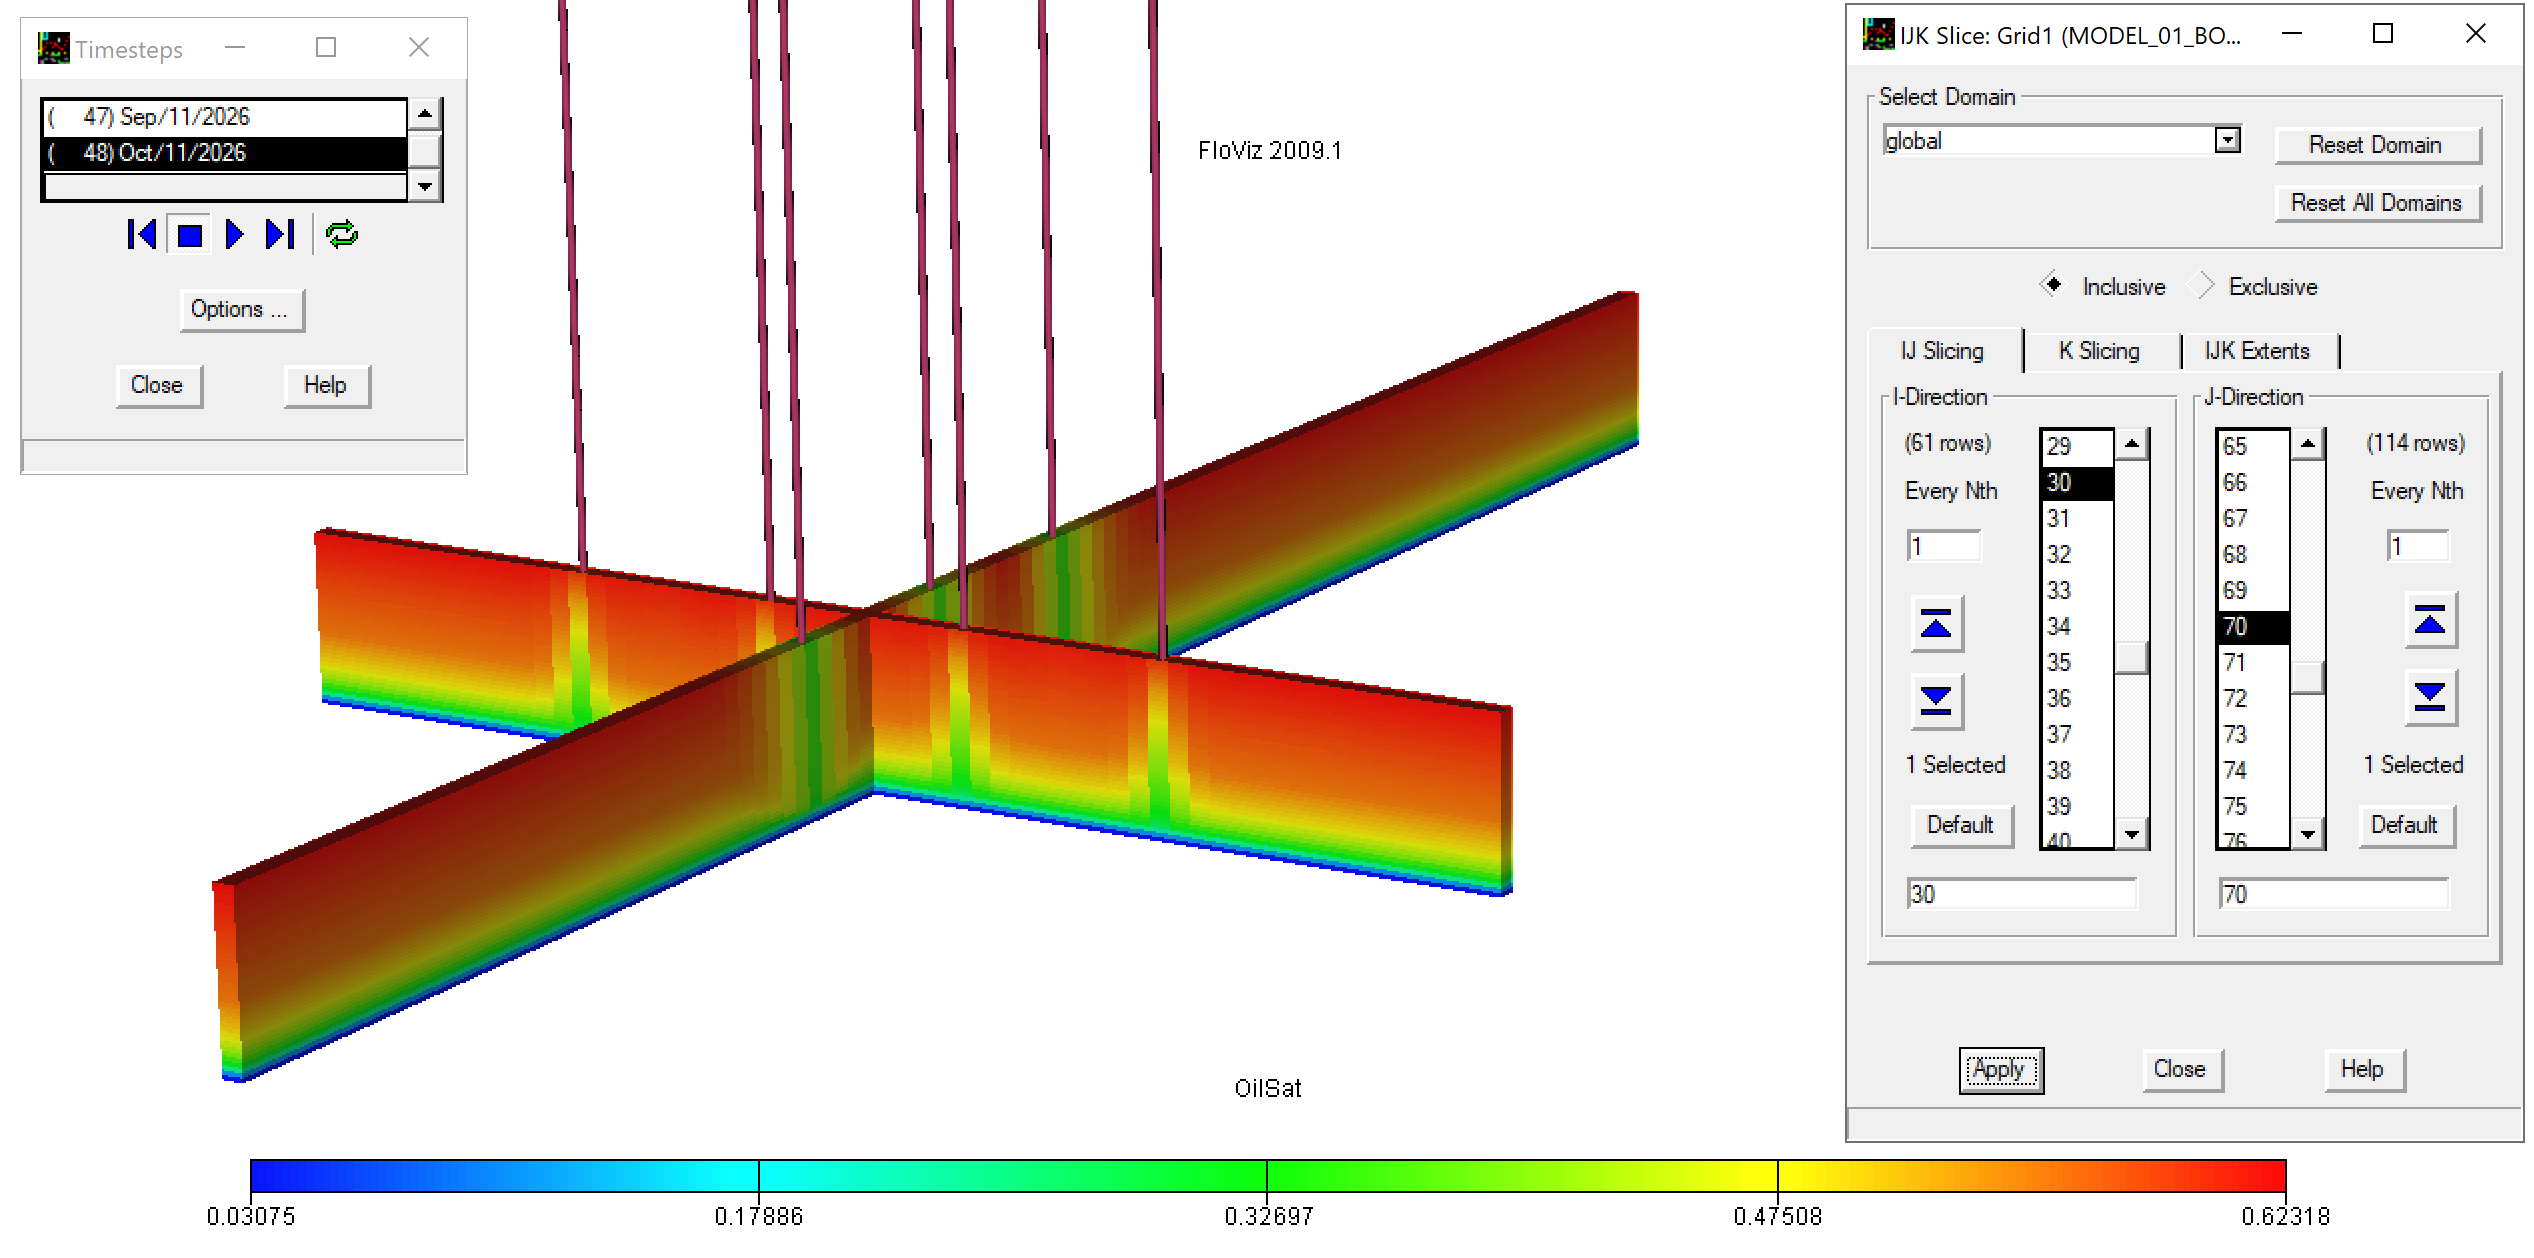
\includegraphics[width=\textwidth]{ecl_oilsat_slices_box_model}
\caption{Нефтенасыщенность в последний месяц моделирования (слайсы вдоль ряда нагнетательных и вдоль ряда добывающих скважин) -- визуализация FloViz}
\label{fig:ecl_oilsat_slices_box_model}
\end{figure}


\begin{figure}[H]
\center
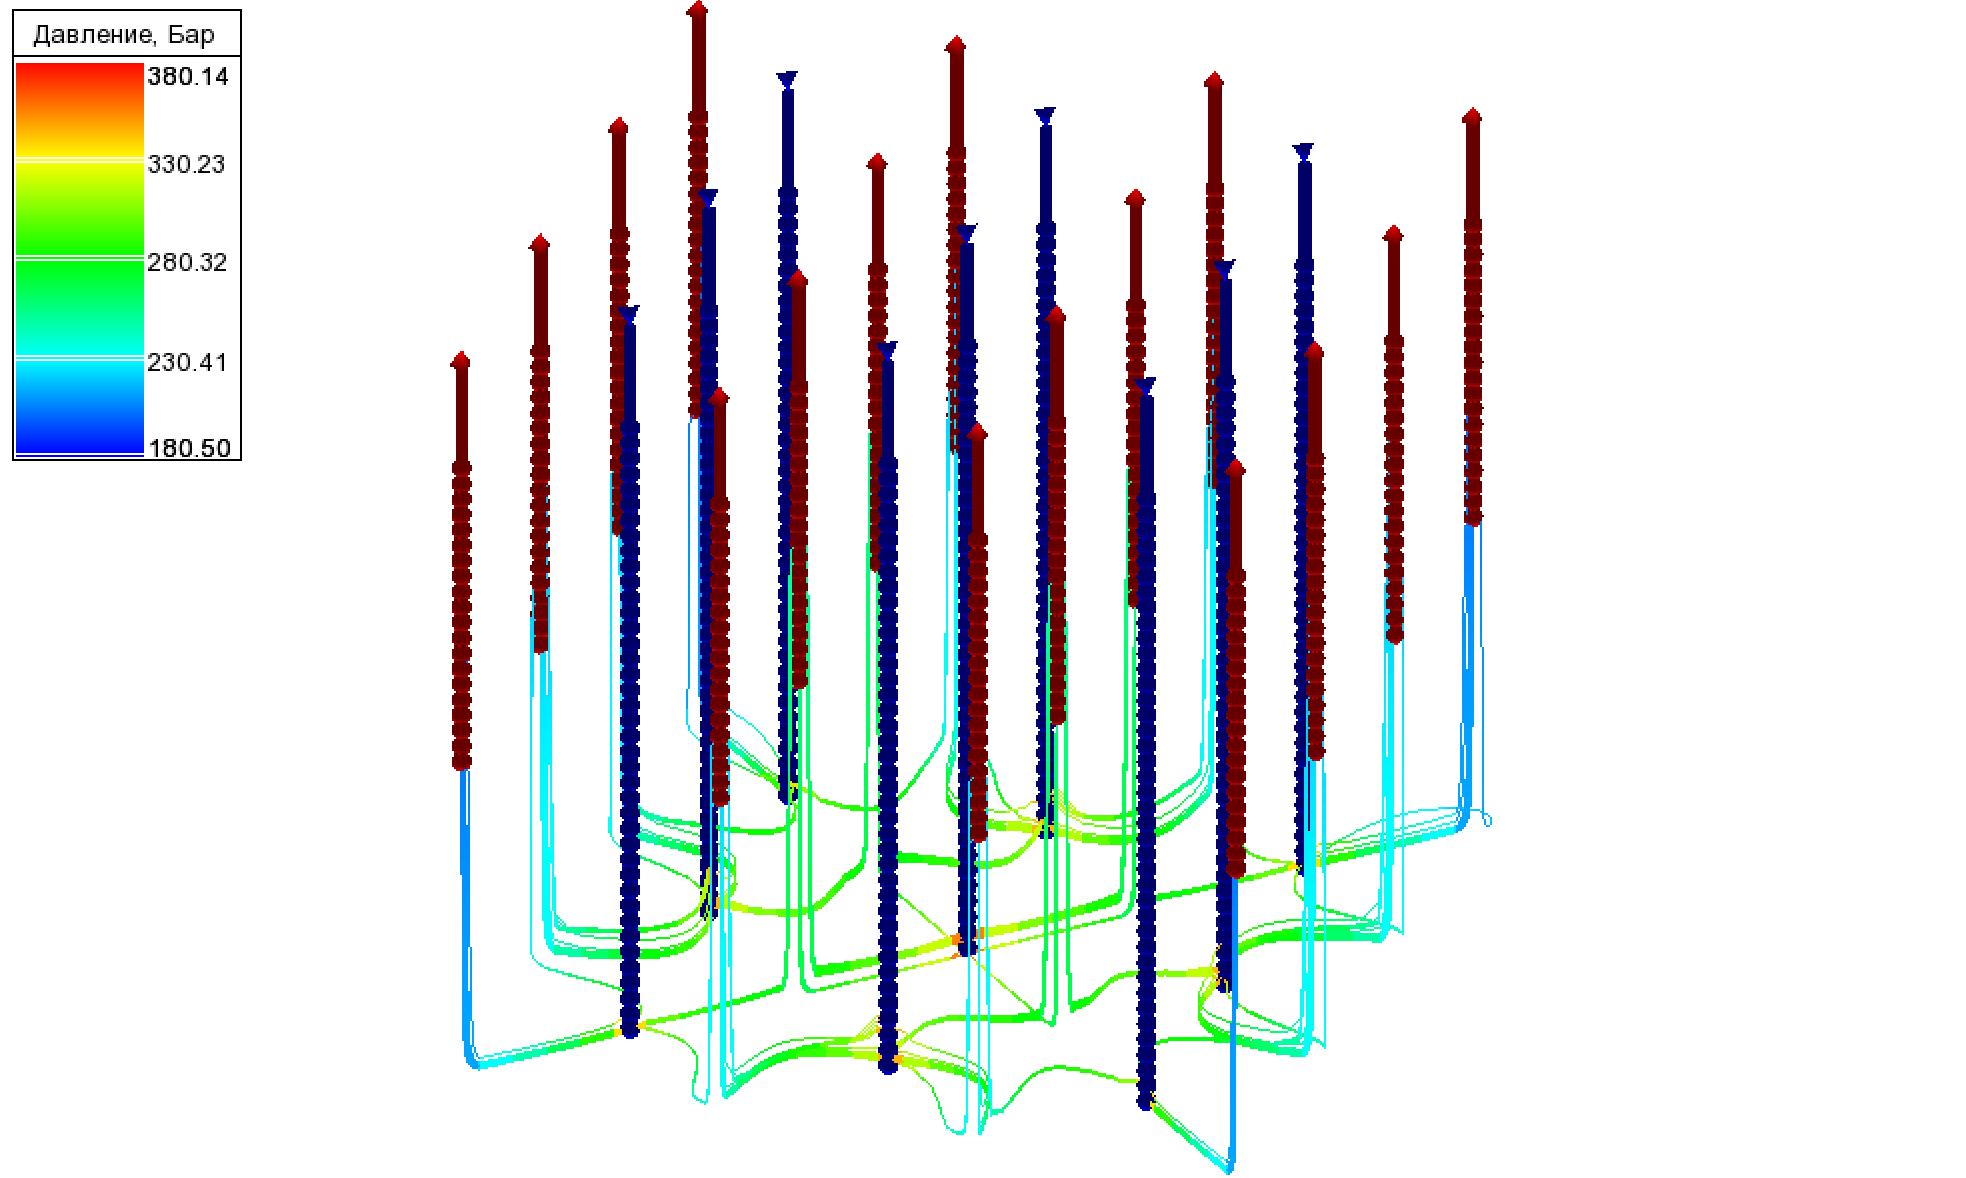
\includegraphics[width=\textwidth]{tnav_flow_lines_start_box_model}
\caption{Линии тока в первые месяцы расчёта -- визуализация tNavigator}
\label{fig:tnav_flow_lines_start_box_model}
\end{figure}

\begin{figure}[H]
\center
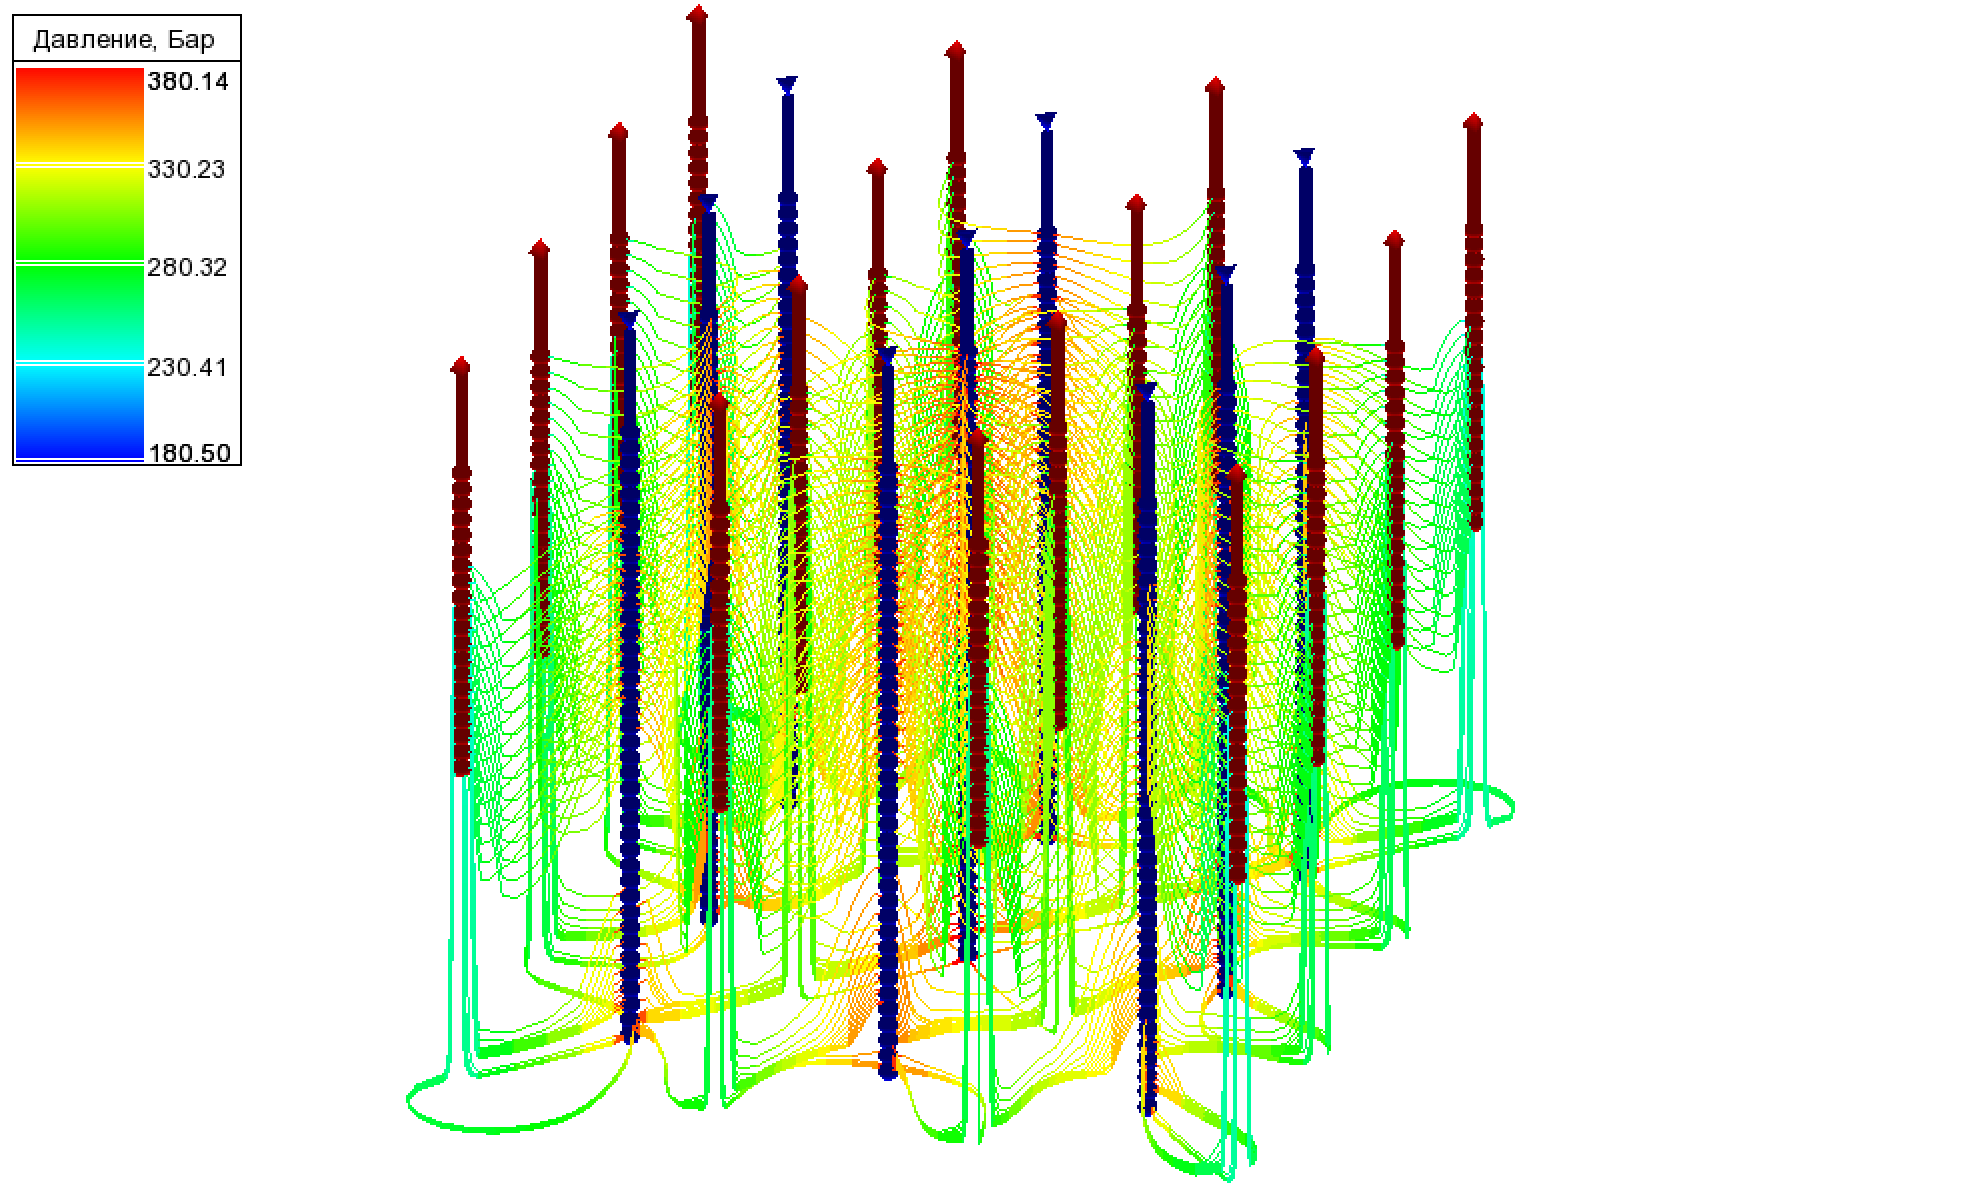
\includegraphics[width=\textwidth]{tnav_flow_lines_end_box_model}
\caption{Линии тока в последний месяц моделирования -- визуализация tNavigator}
\label{fig:tnav_flow_lines_end_box_model}
\end{figure}

\begin{figure}[H]
\center
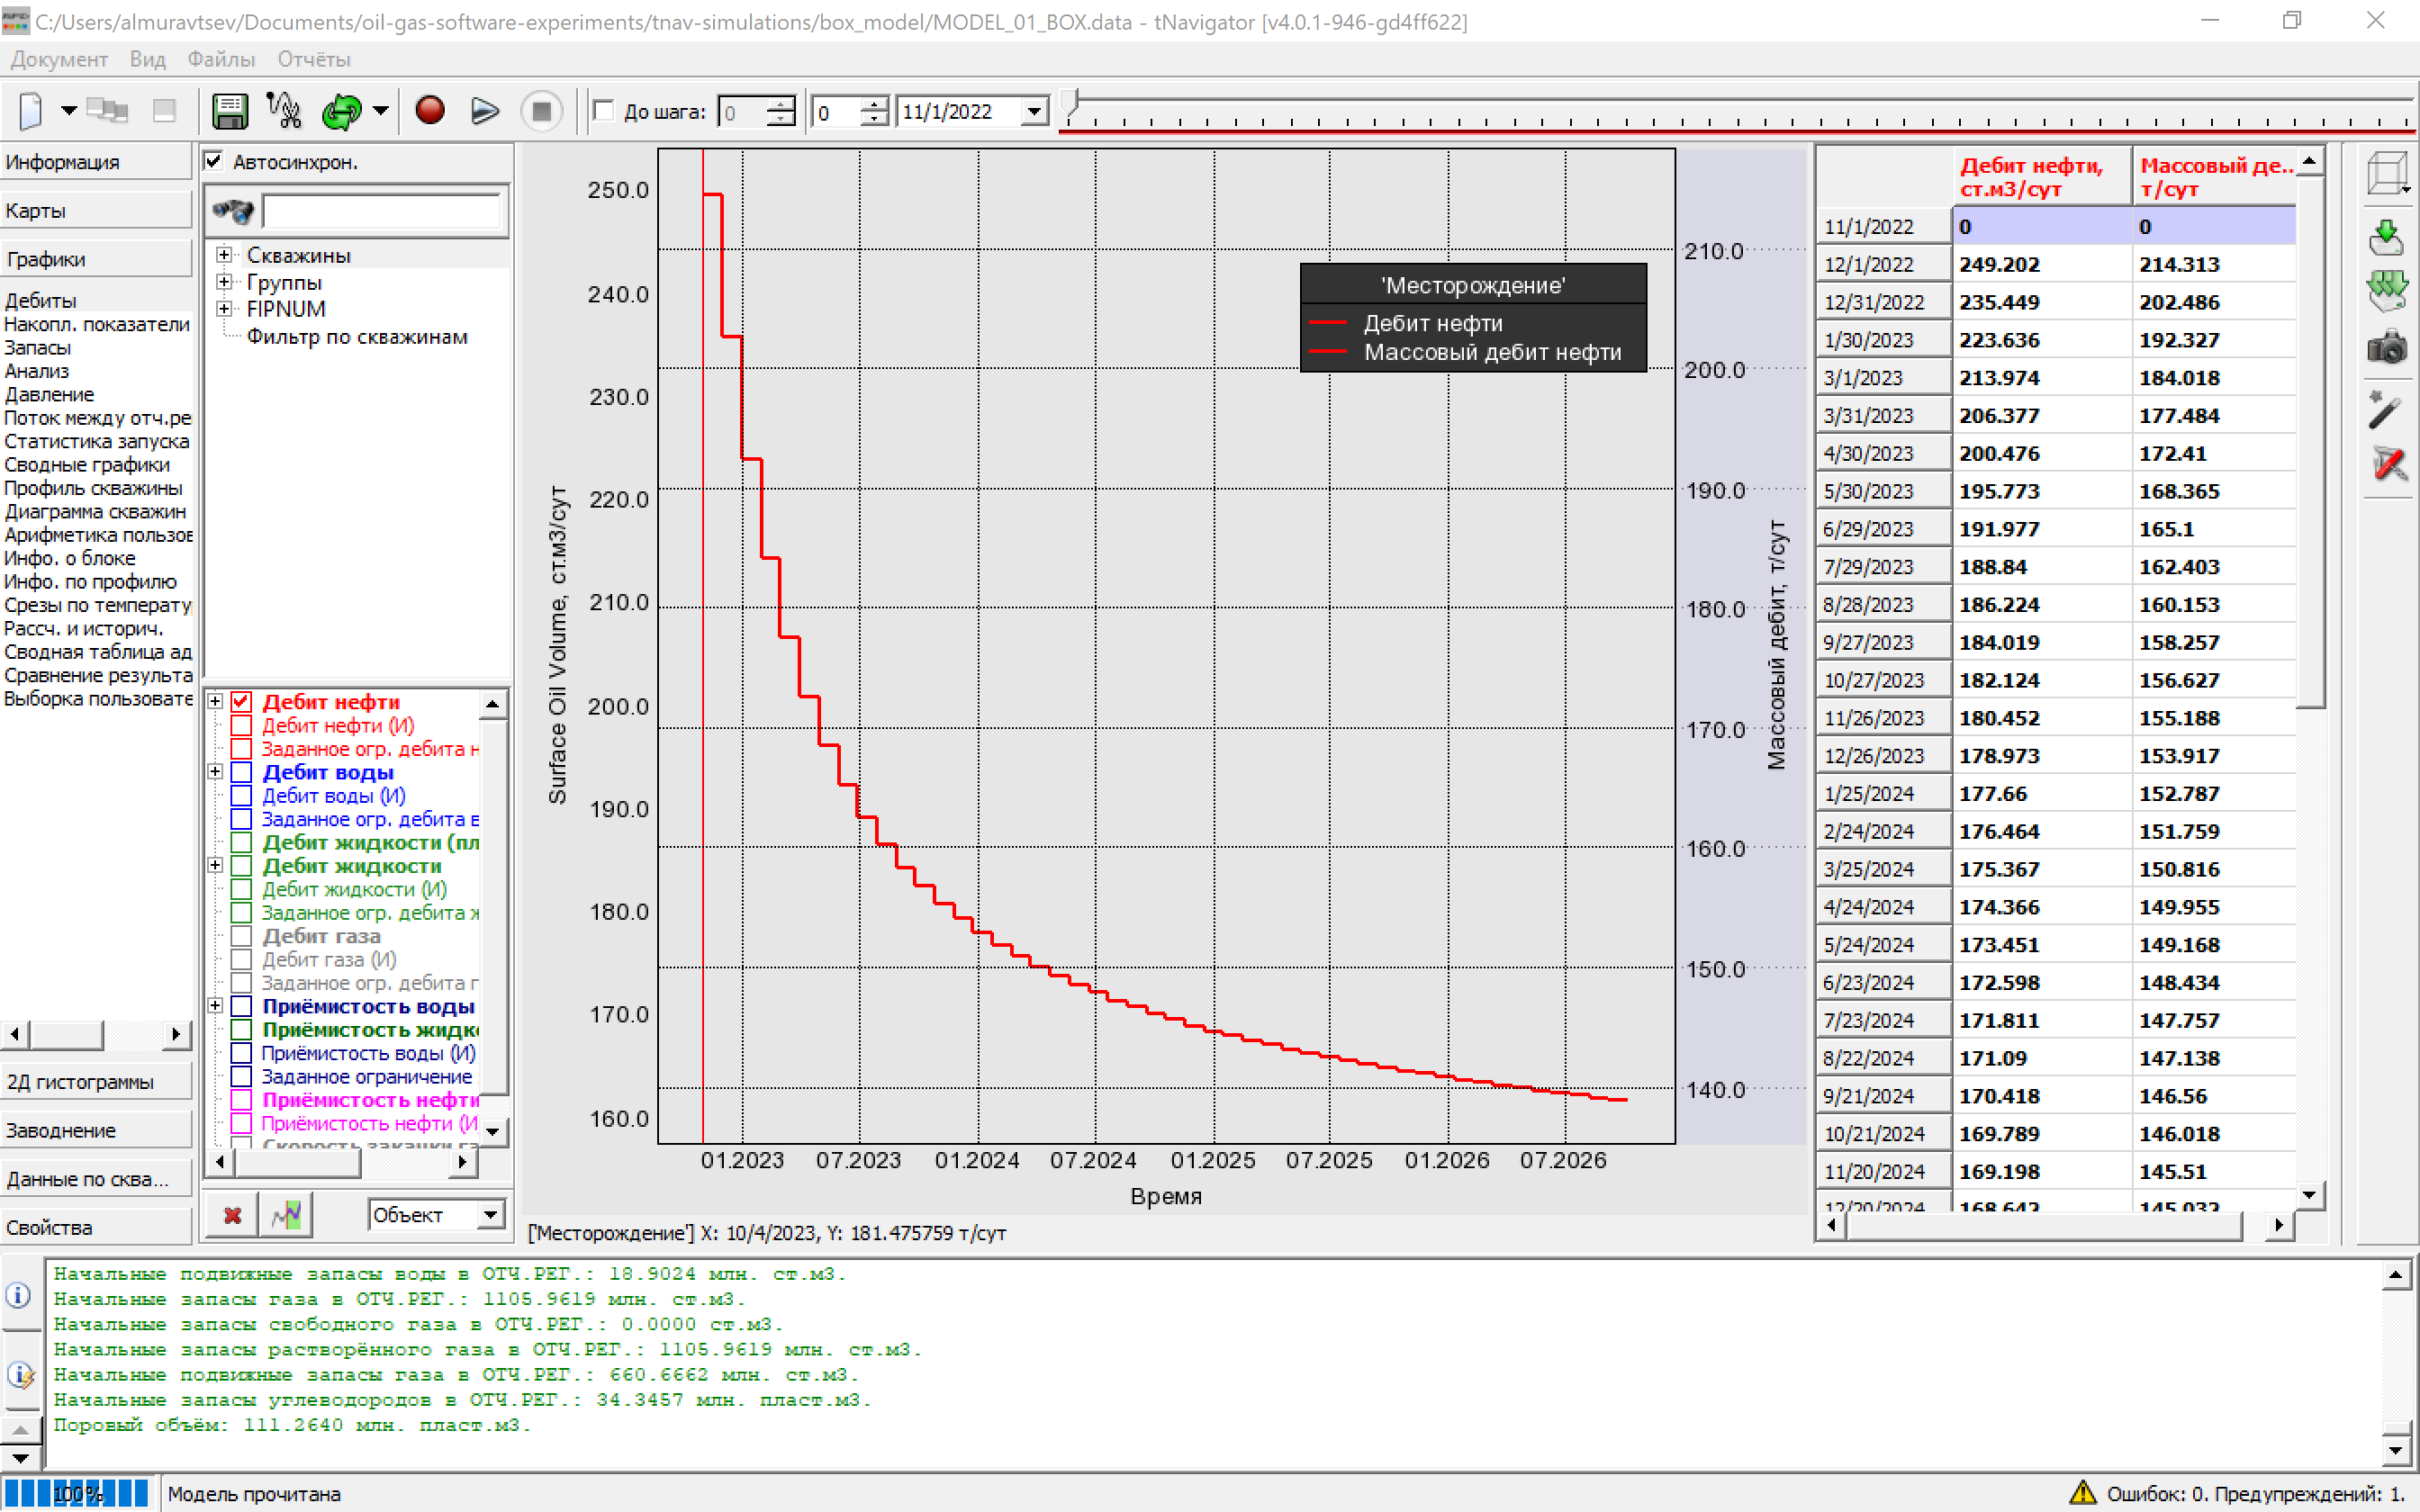
\includegraphics[width=\textwidth]{tnav_fopr_box_model}
\caption{График дебитов нефти (суммарно со всех скважин)-- визуализация tNavigator}
\label{fig:tnav_fopr_box_model}
\end{figure}

\begin{figure}[H]
\center
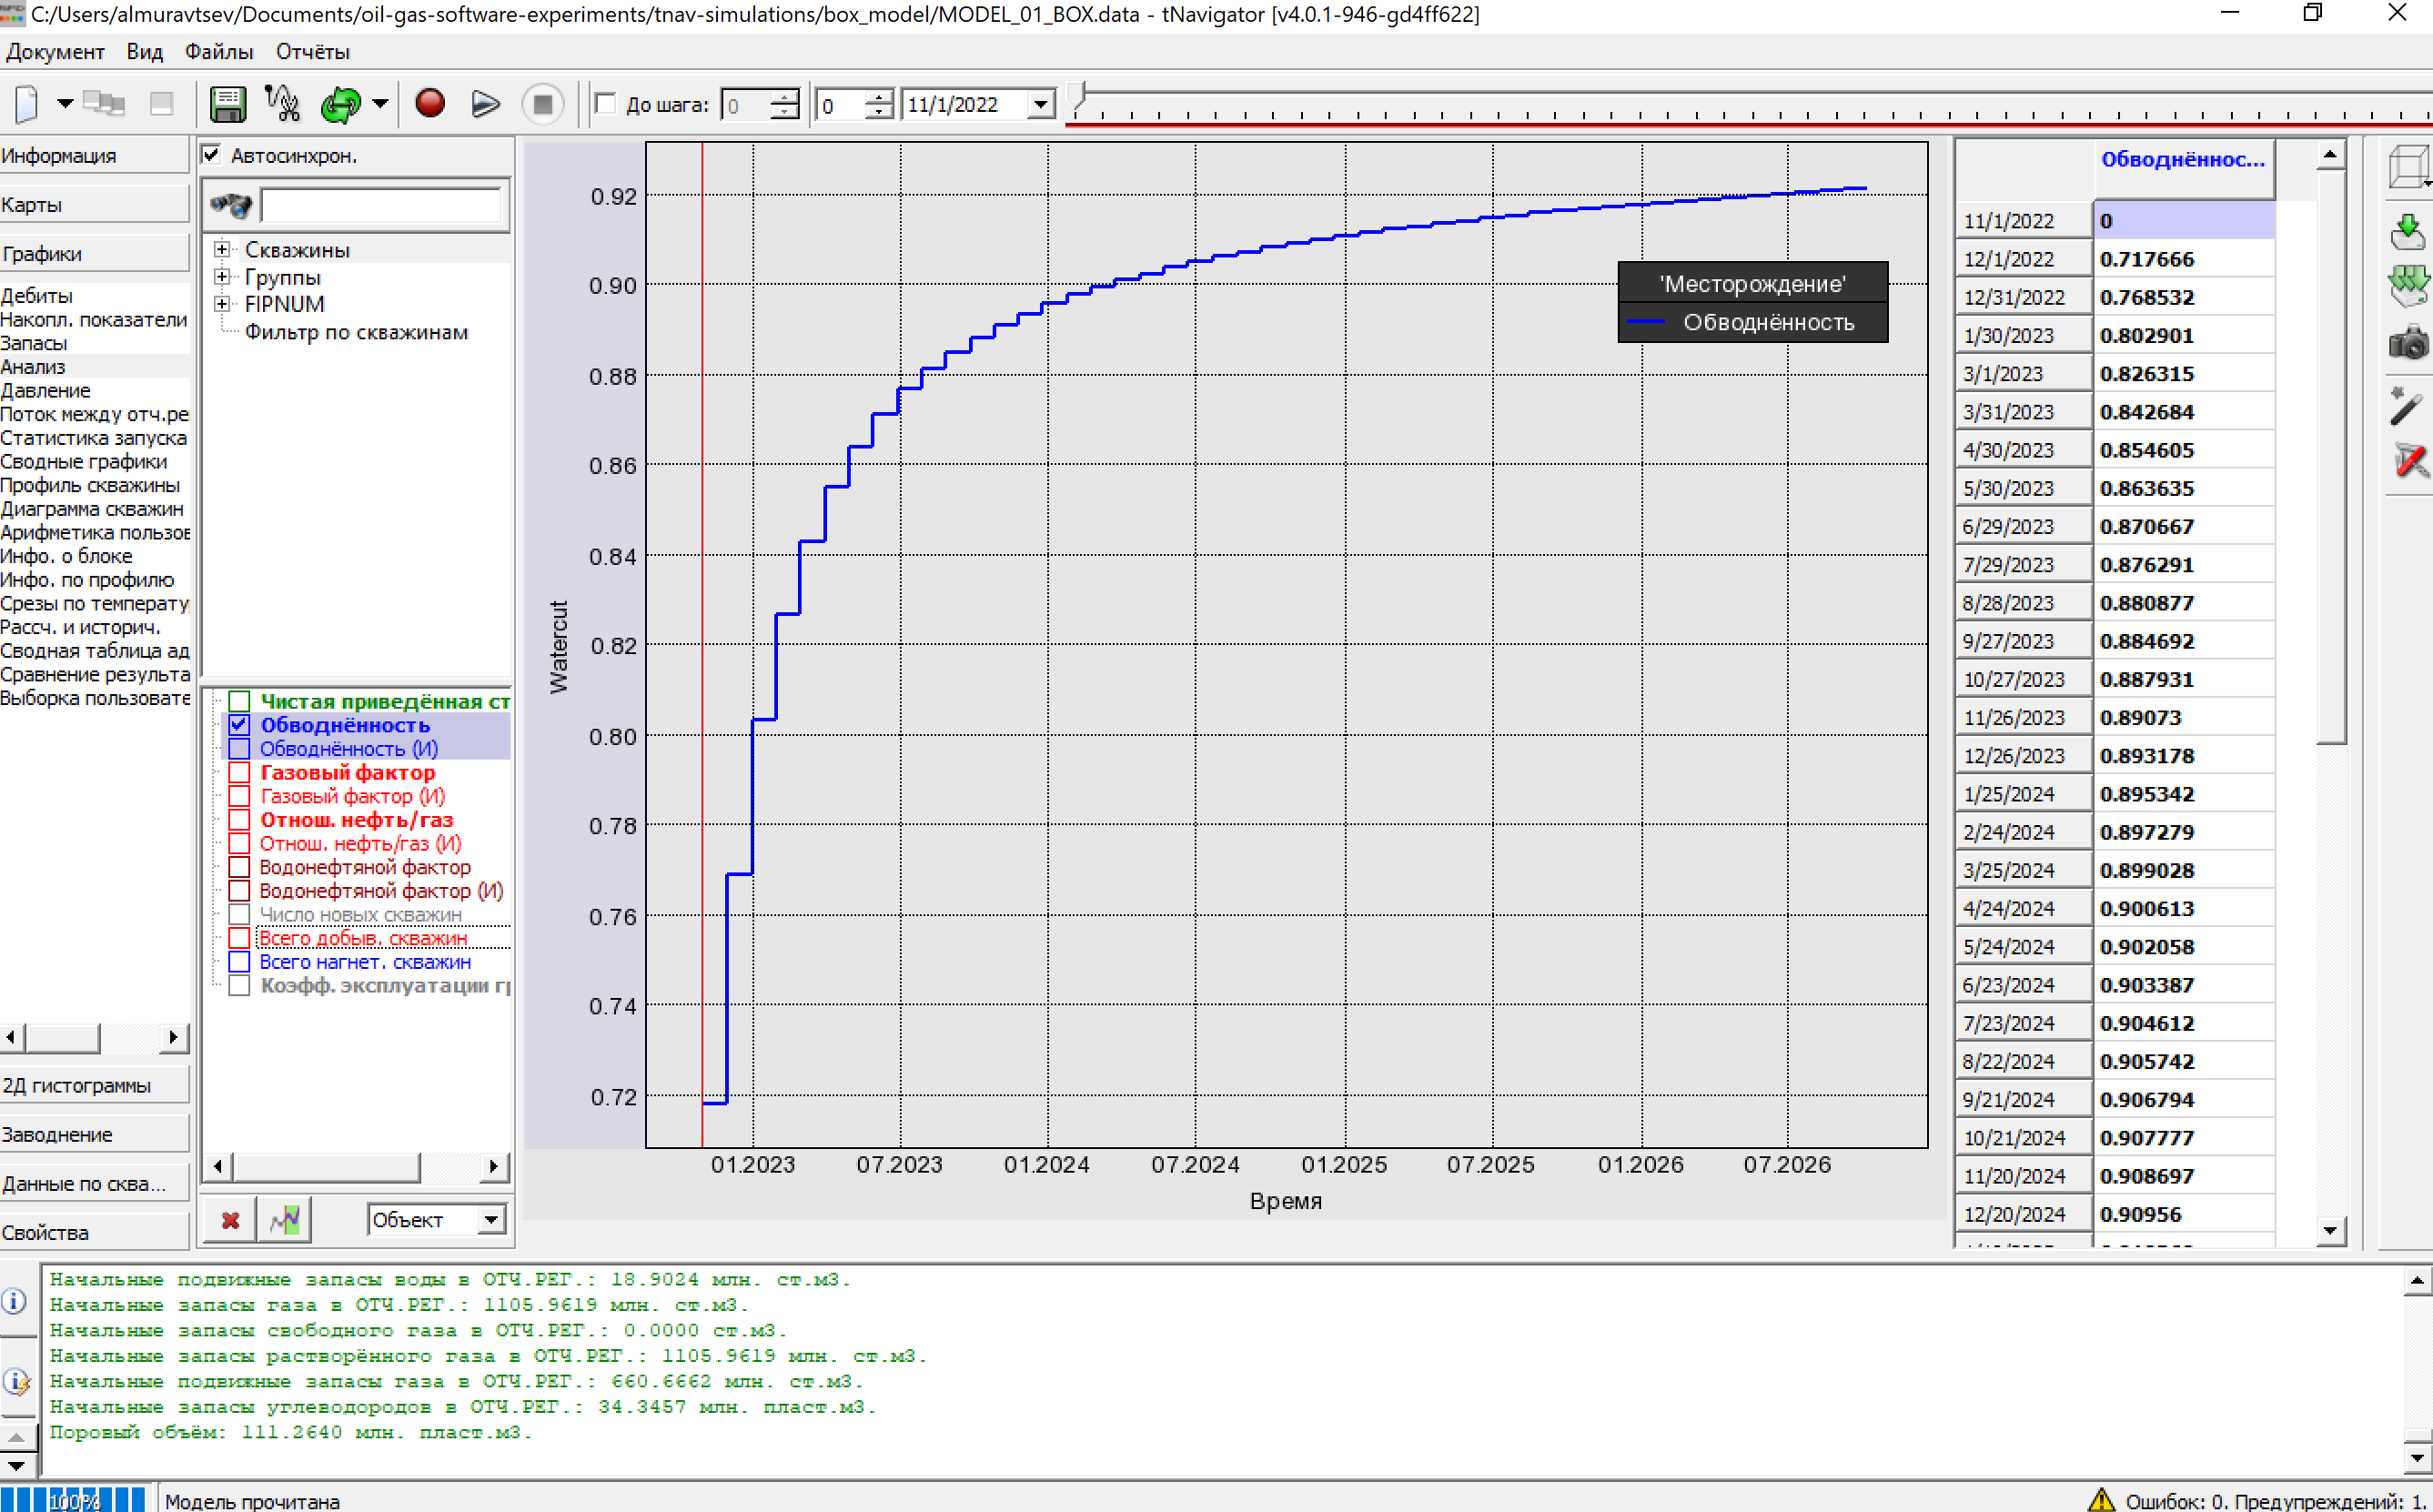
\includegraphics[width=\textwidth]{tnav_fwct_box_model}
\caption{График обводнённости (суммарно со всех скважин) -- визуализация tNavigator}
\label{fig:tnav_fwct_box_model}
\end{figure}


\begin{figure}[H]
\center
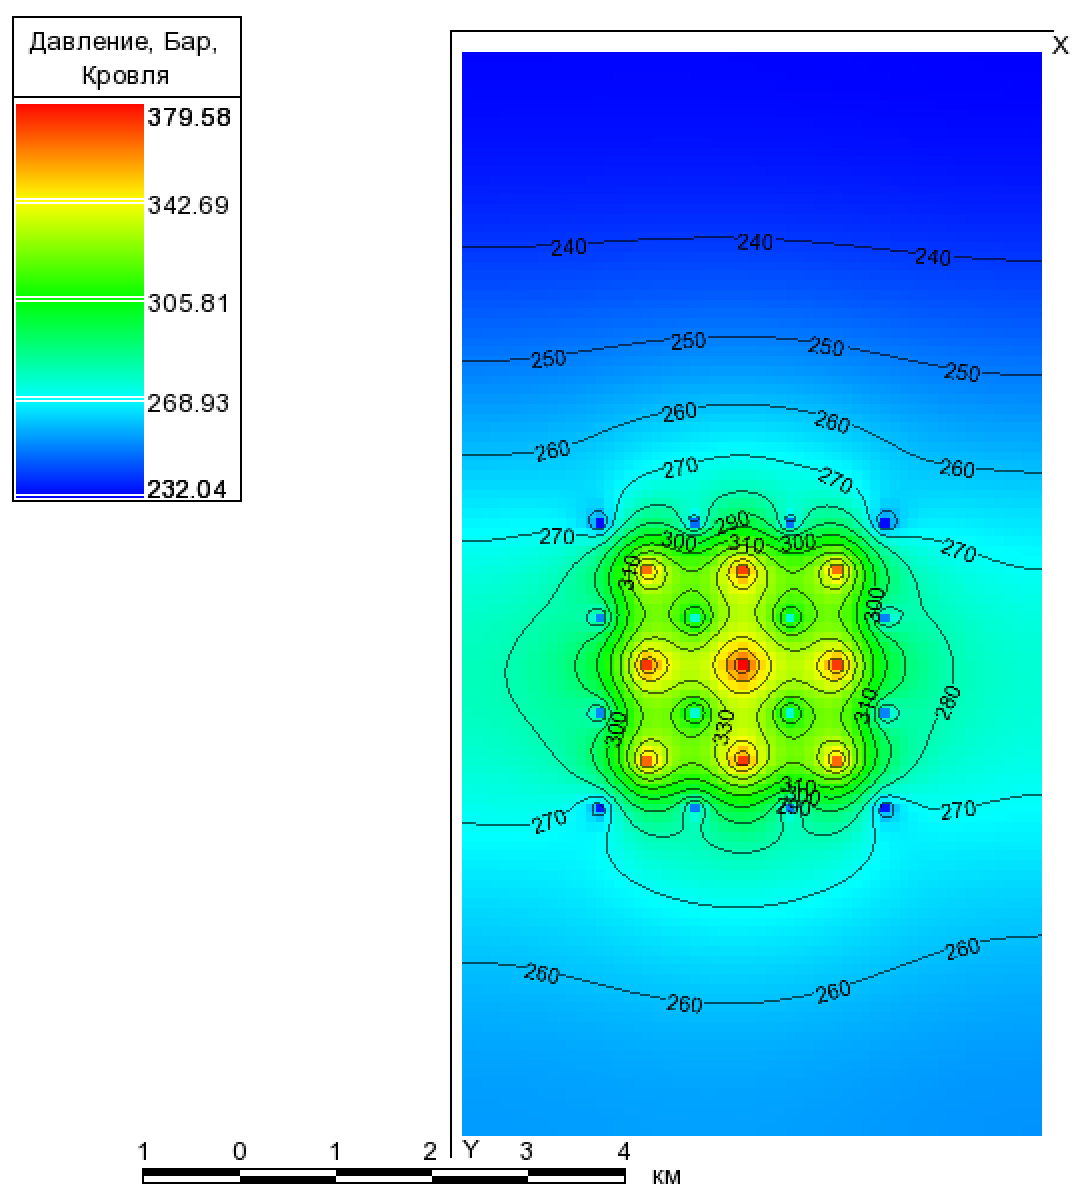
\includegraphics[width=.6\textwidth]{tnav_head_box_pressure_map}
\caption{Распределение давления -- визуализация tNavigator}
\label{fig:tnav_fwct_box_model}
\end{figure}


\newpage
\section{Задание от 05.10.2022}

\begin{enumerate}
	\item Требуется дополнить модель из задания от 28.09.2022 гридами структуры, пористости, активных ячеек
	\item Проницаемость задать по зависимости от пористости (по керну), анизотропию проницаемости по керну, ЗСВ 1252 м
	\item Проинициализировать модель различными способами:
	\begin{itemize}
		\item EQUIL + Pc (задать различные величины Pc на контакте)
		\item EQUIL + SWATINIT
		\item Понять как меняется начальное распределение насыщенности (и запасы) в модели в зависимости от способа инициализации
	\end{itemize}
\end{enumerate}

\subsection{Дополнение модели гридами структуры, пористости, активных ячеек}

В секции \textbf{RUNSPEC} изменим максимальное число водоносных пластов, описанных с помощью аналитической модели (увеличим от 1 до 3).
\begin{eclrun}
AQUDIMS
  4*  3  100000 /
\end{eclrun}

Полностью перепишем секцию \textbf{GRID} предыдущей модели от 28.09.2022.

В начале секции \textbf{GRID} пропишем ключевое слово NEWTRAN, чтобы показать, что коэффициенты пропускания рассчитываются по угловым положениям ячеек (типично при задании геометрии угловой точки).
\begin{eclrun}
NEWTRAN
\end{eclrun}

Дополнительно будем использовать опциональное ключевое слово NOECHO с целью уменьшения количества выводов в консоль и для предотвращения вывода больших прилагаемых файлов.
\begin{eclrun}
NOECHO
\end{eclrun}

Подключим файл с гридом структуры.
Геометрия сгененерирована в Petrel-е и задана в виде геометрии угловой точки (с помощью ключевых слов COORD и ZCORN).
\begin{eclrun}
INCLUDE
'INC\GRID.inc' /
\end{eclrun}

Подключим файл с гридом активных ячеек, в котором с помощью ключевого слова ACTNUM прописаны активные ячейки (файл сгенерирован в т-Навигаторе).
\begin{eclrun}
INCLUDE
'INC\ACTNUM.inc' /
\end{eclrun}

Подключим файл с гридом пористости PORO (файл сгенерирован в т-Навигаторе).
\begin{eclrun}
INCLUDE
'INC\PORO.inc' /
\end{eclrun}


\begin{figure}[H]
\center
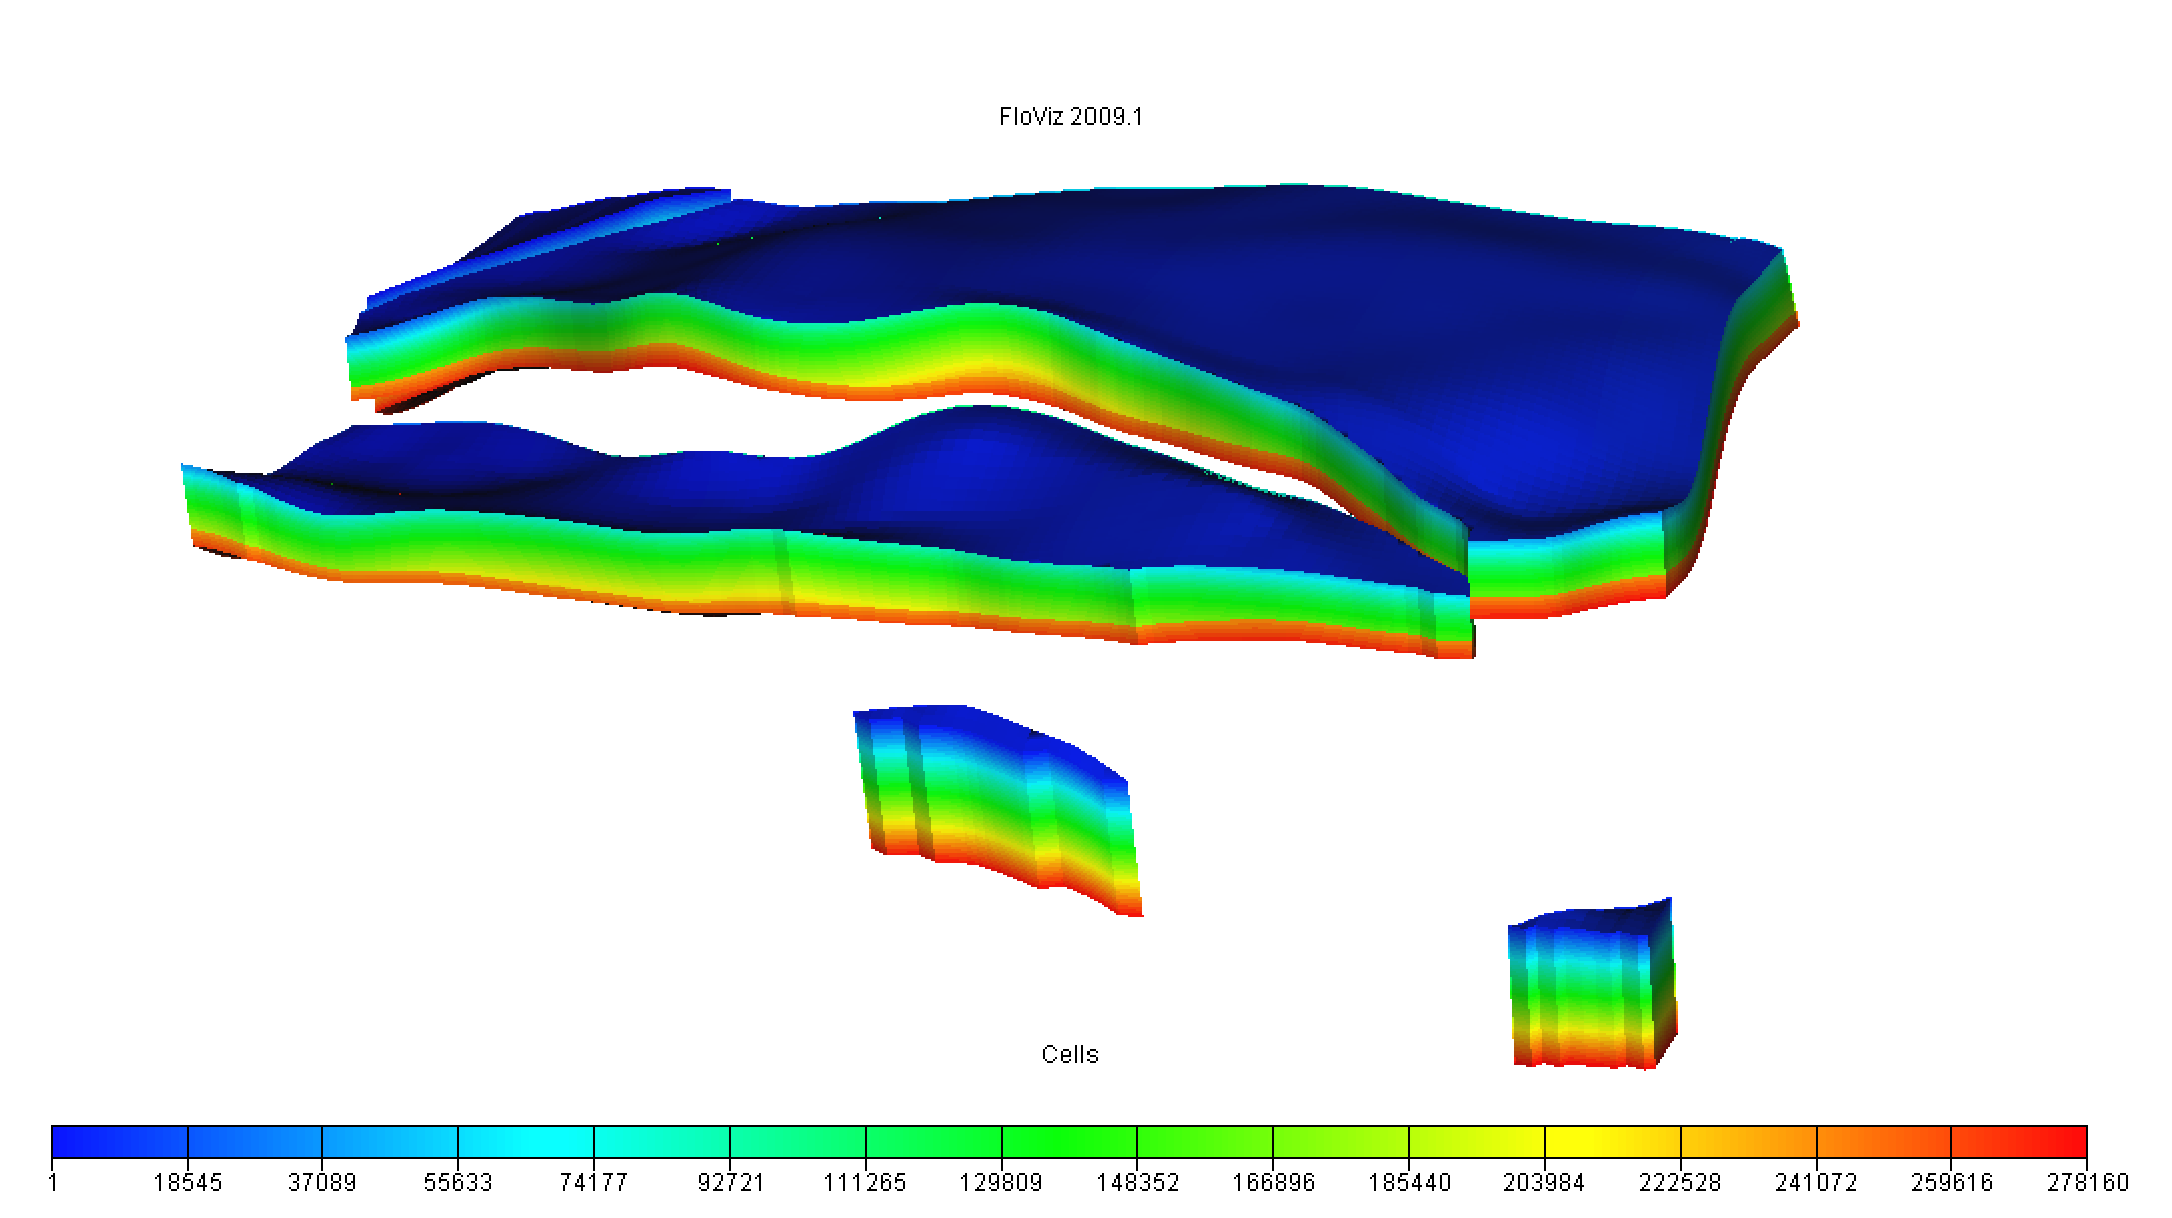
\includegraphics[width=\textwidth]{ecl_grid_cells_model_01}
\caption{Грид структуры (все ячейки) модели -- визуализация FloViz}
\label{fig:ecl_grid_cells_model_01}
\end{figure}


\begin{figure}[H]
\center
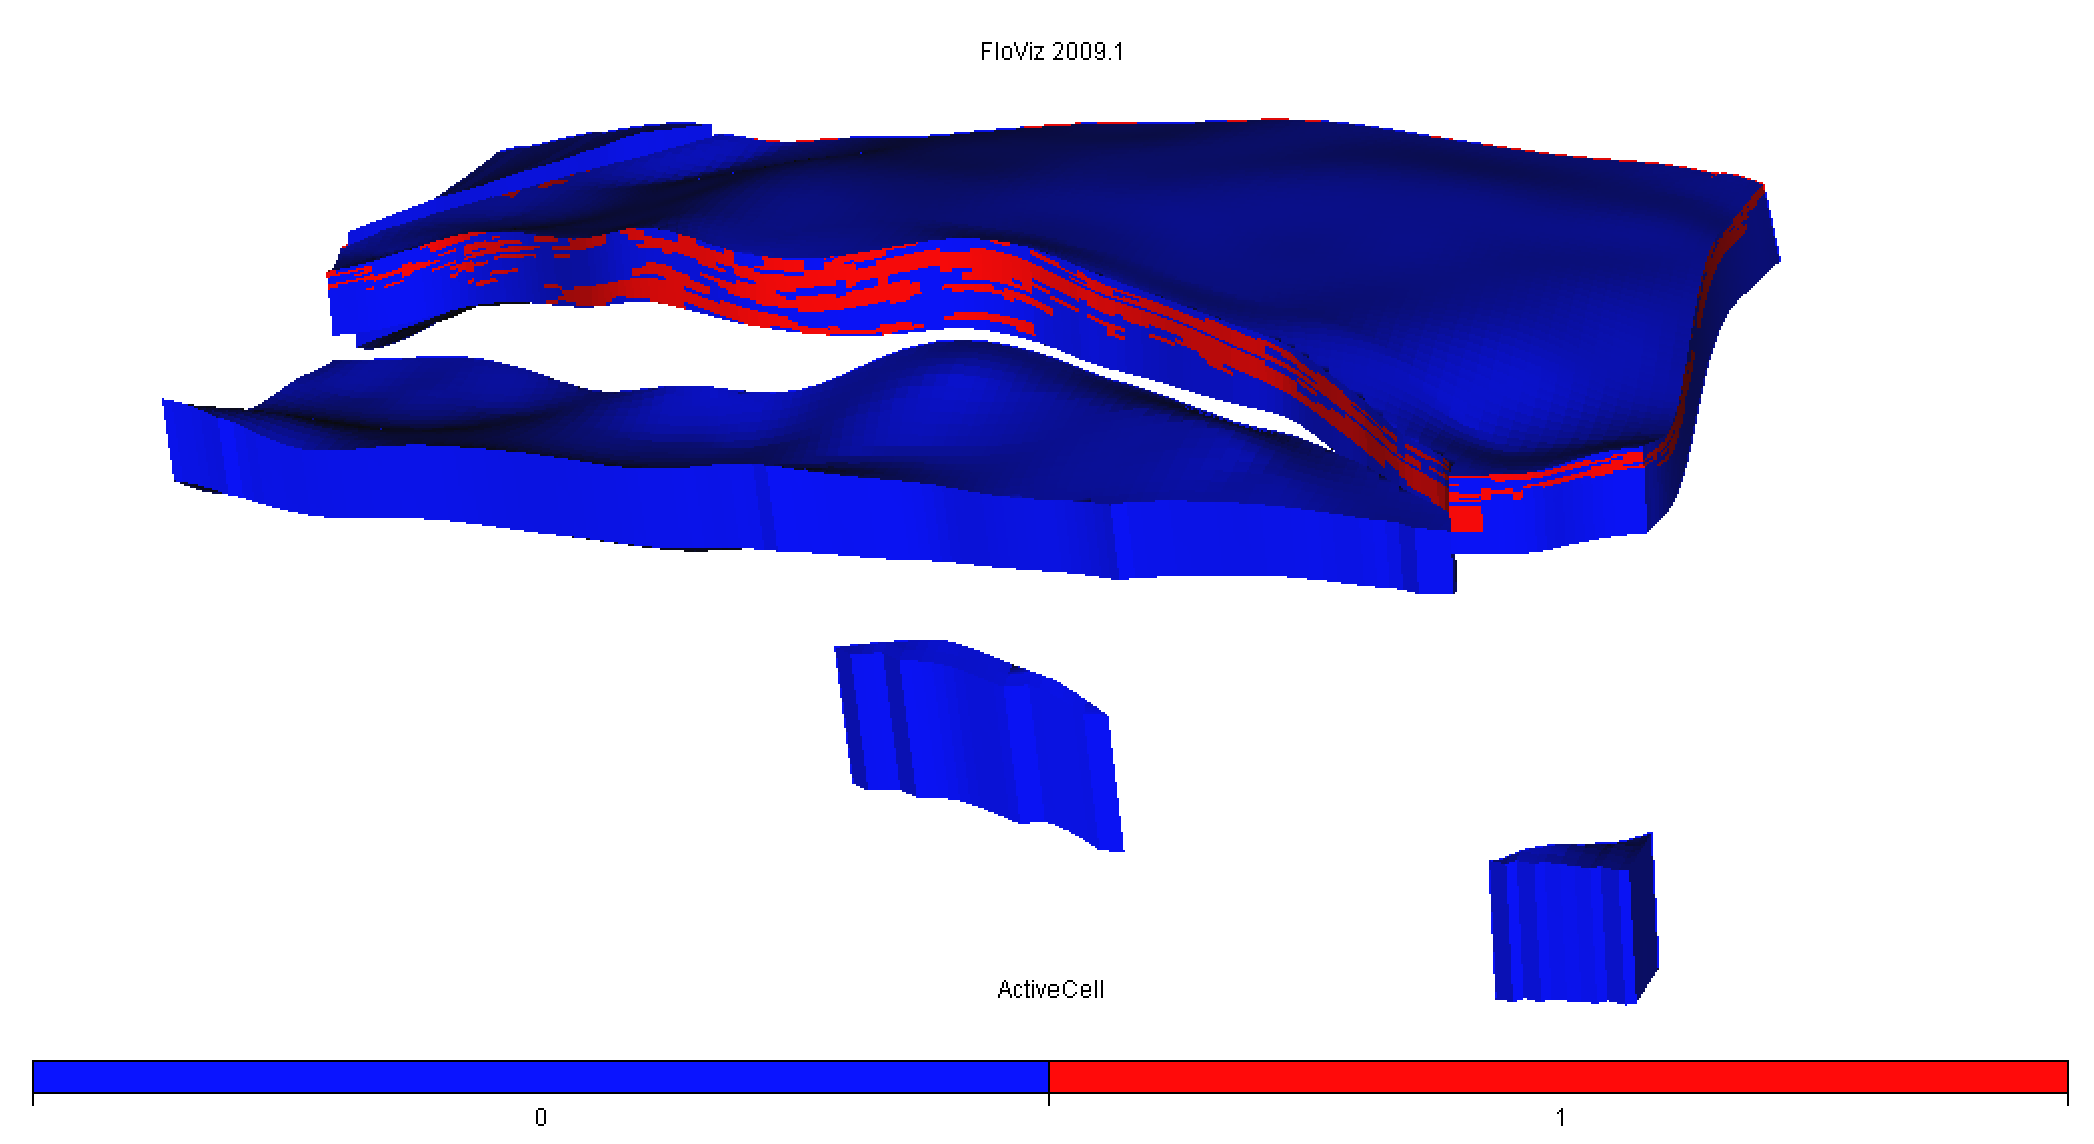
\includegraphics[width=\textwidth]{ecl_grid_active_cells_model_01}
\caption{Грид активных ячеек модели -- визуализация FloViz}
\label{fig:ecl_grid_active_cells_model_01}
\end{figure}


\begin{figure}[H]
\center
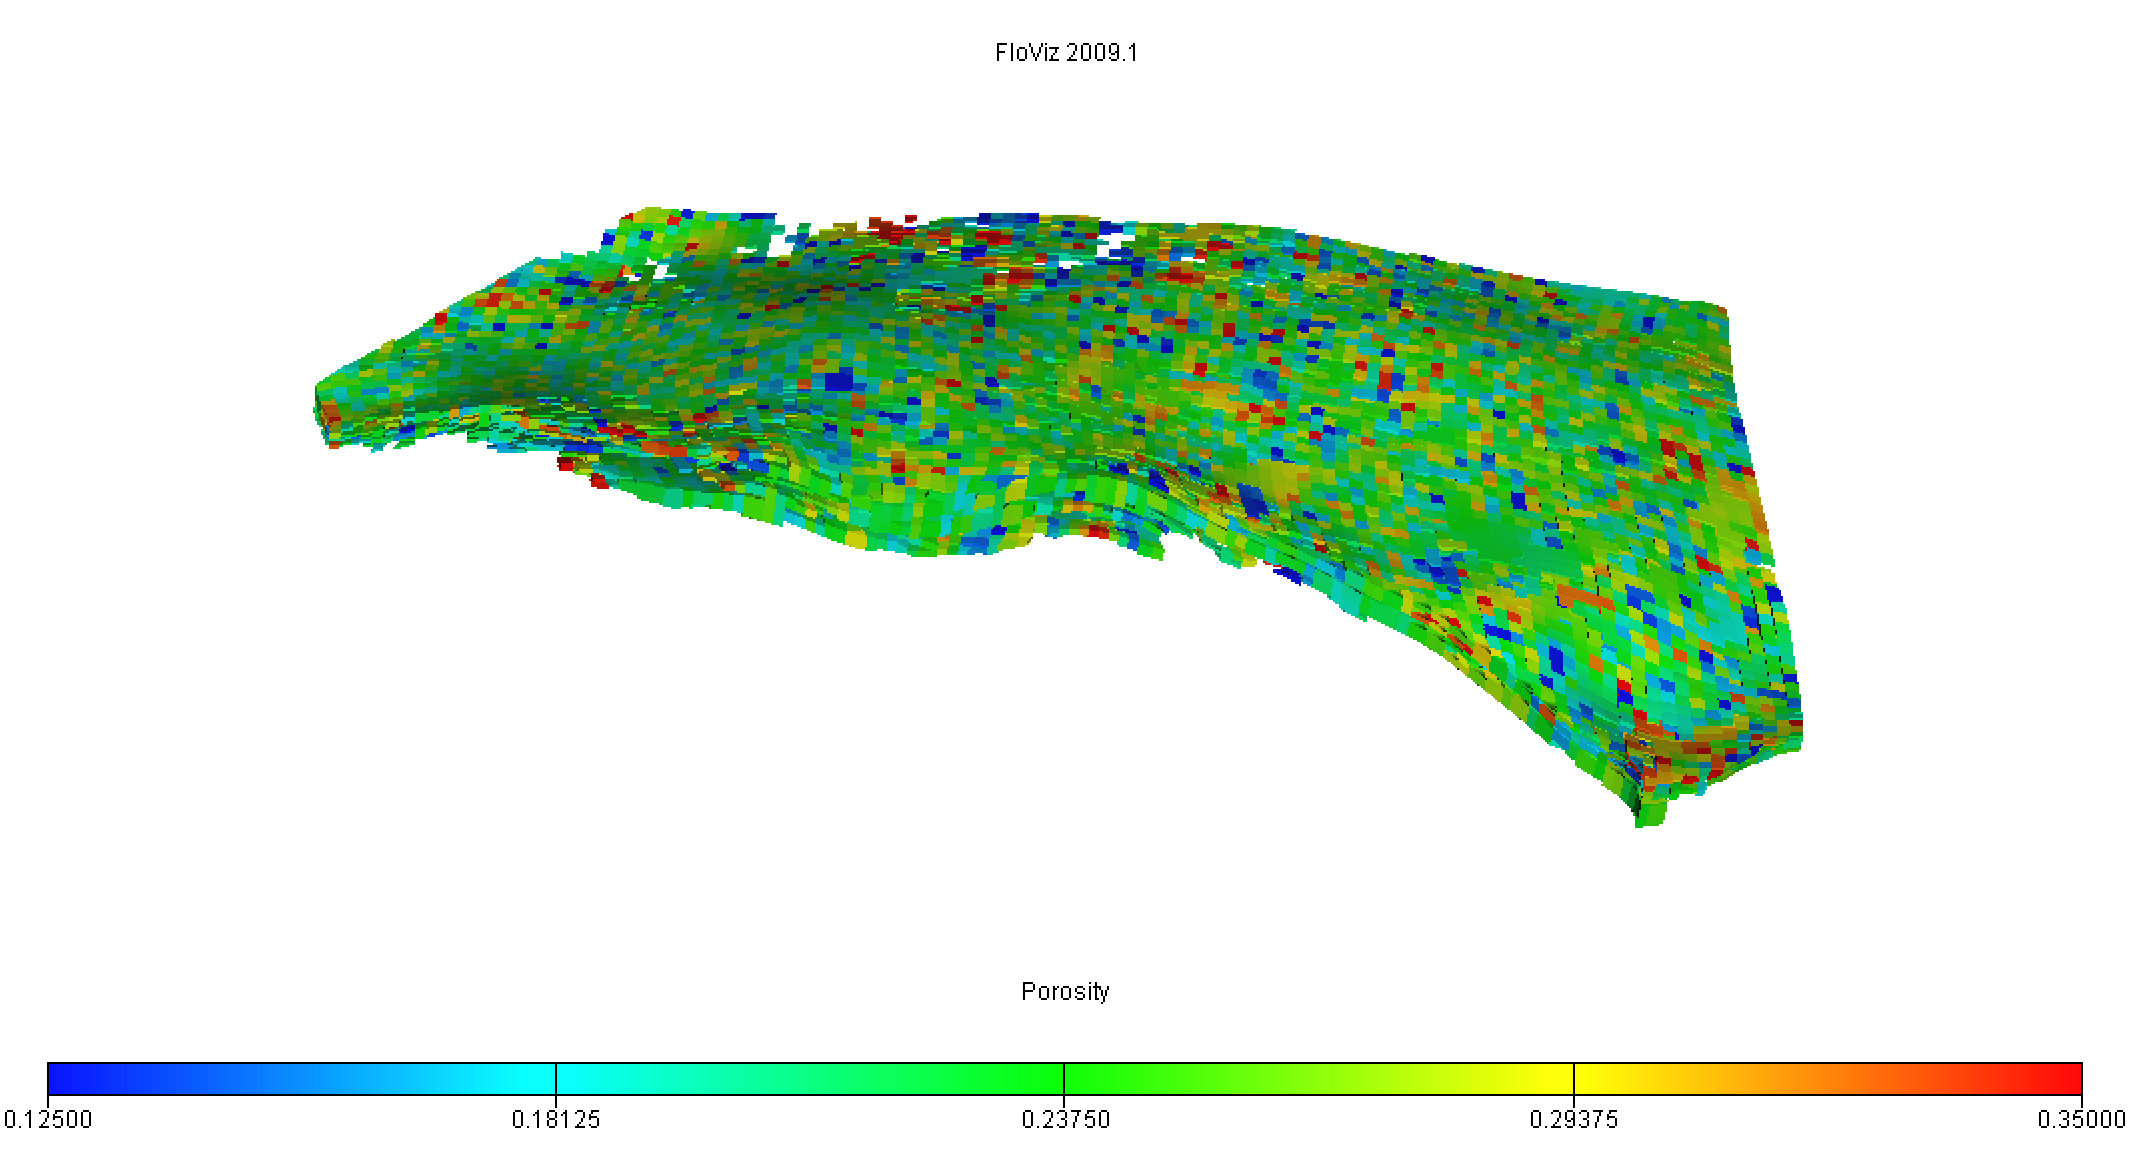
\includegraphics[width=\textwidth]{ecl_poro_model_01}
\caption{Грид пористости (только для активных ячеек) -- визуализация FloViz}
\label{fig:ecl_poro_model_01}
\end{figure}

В секции \textbf{REGION} укажем регионы (области, пласты) модели.
\begin{eclrun}
EQUALS
FIPNUM 1  1 61  1 114   1 17 /--RESERVOIR 1
FIPNUM 2  1 61  1 114  18 34 /--RESERVOIR 2
FIPNUM 3  1 61  1 114  35 40 /--RESERVOIR 3
/
\end{eclrun}


\begin{figure}[H]
\center
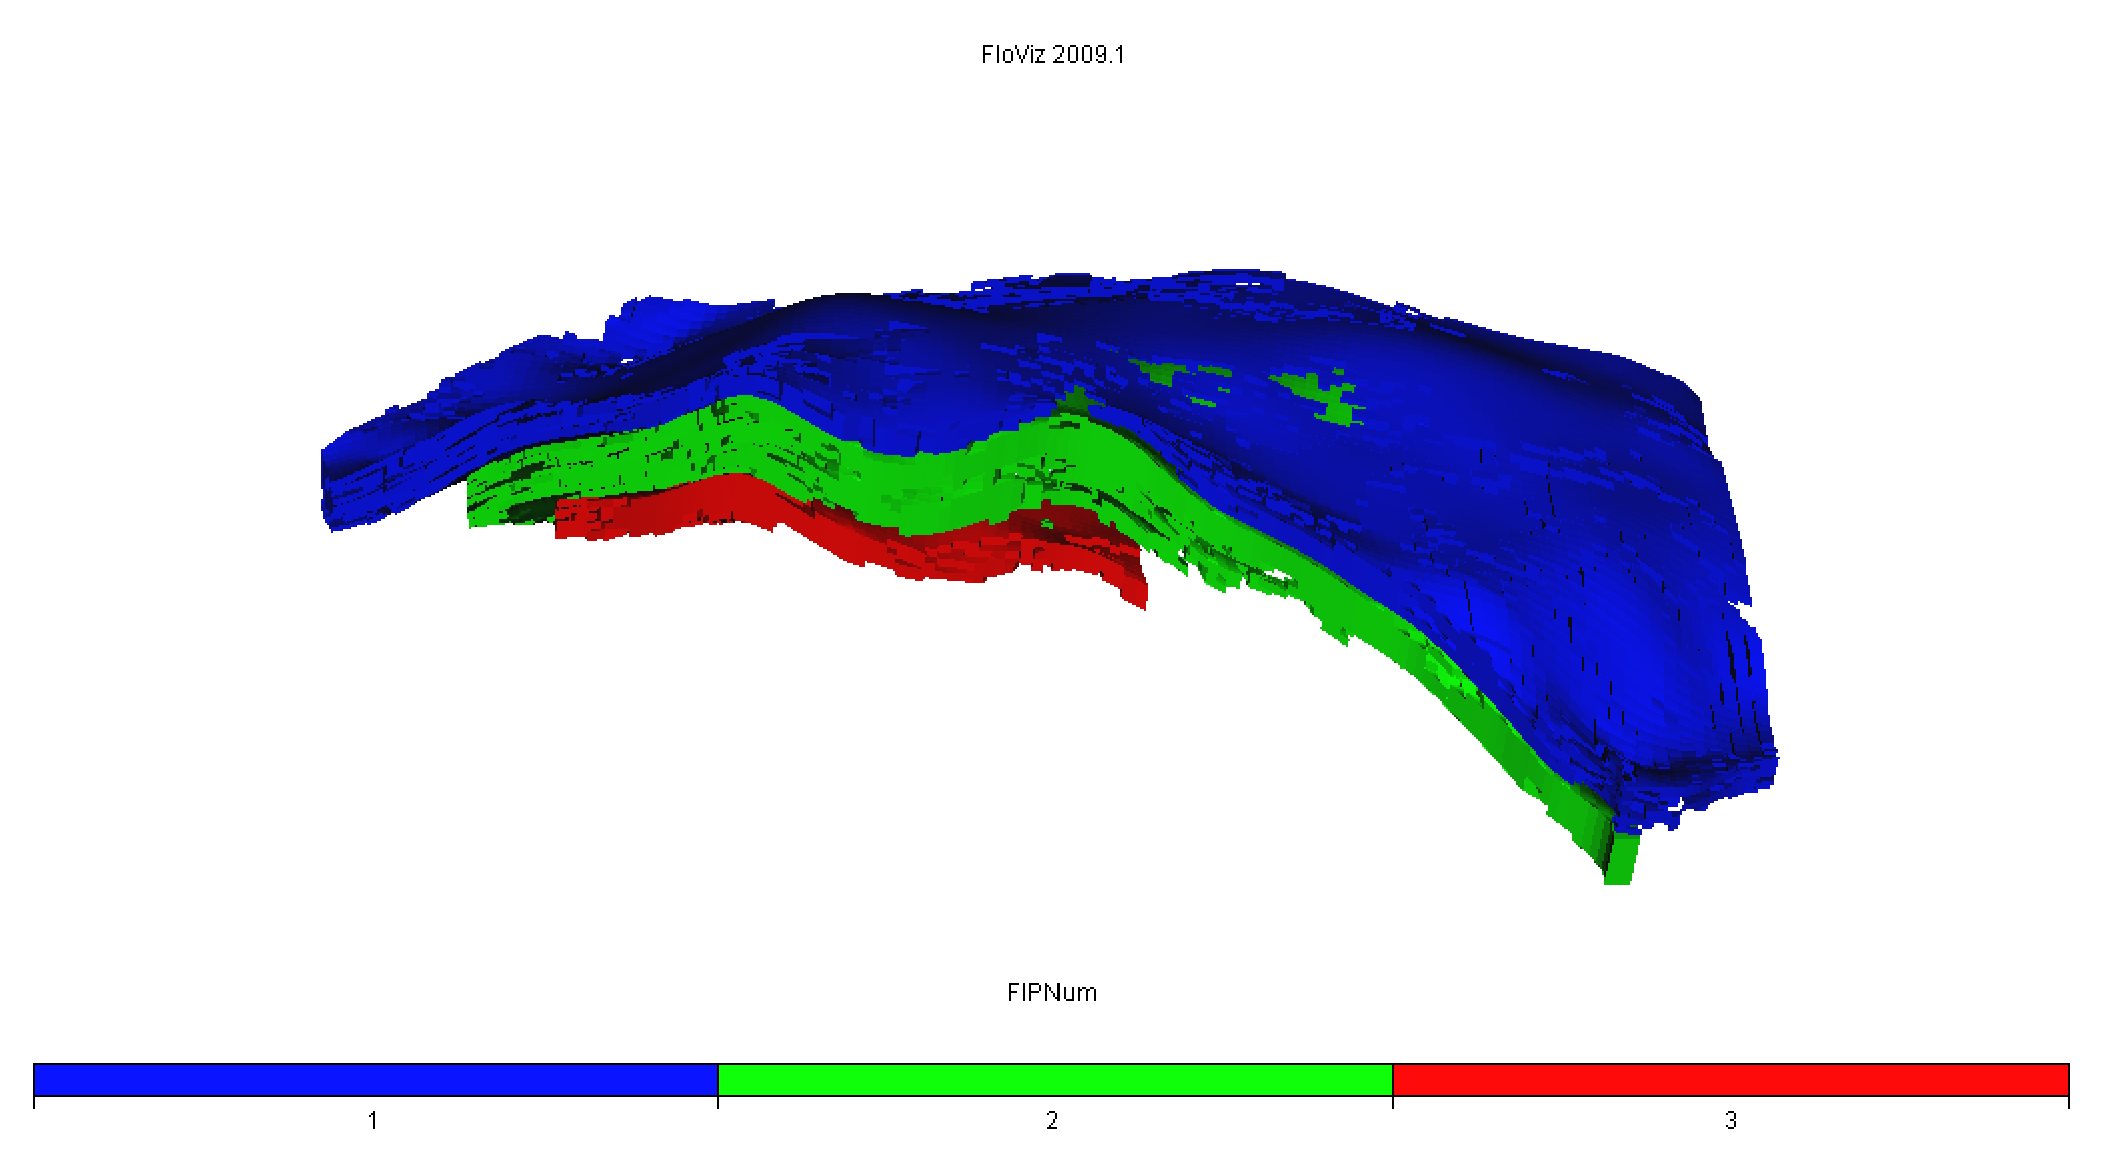
\includegraphics[width=\textwidth]{ecl_fipnum_model_01}
\caption{Регионы модели (только для активных ячеек) -- визуализация FloViz}
\label{fig:ecl_fipnum_model_01}
\end{figure}


\subsection{Задание проницаемости, анизотропии проницаемости}

В секции \textbf{GRID} укажем минимально возможное значение пористости в модели и зададим проницаемость в зависимости от пористости.
\begin{eclrun}
EQUALS
PERMX 1 /
/

MINVALUE
PORO 0.00001 /
/

OPERATE
PERMX  1 61  1 114  1 40  'MULTP'  PORO  14593.4635  2.62189 /
/

COPY
PERMX PERMY /
PERMX PERMZ /
/
\end{eclrun}

Зададим анизотропию проницаемости.
\begin{eclrun}
MULTIPLY
PERMZ  0.499 /--Kv/Kh RATIO
/
\end{eclrun}

Скажем симулятору, что необходимо записать исходные данные со свойствами сетки и таблицами насыщенностей в файл, который в дальнейшем можно будет прочесть в графических пакетах.
\begin{eclrun}
INIT
\end{eclrun}

Далее в начале секции \textbf{SOLUTION} зададим приток из аквифера, рассчитанный по модели Картера-Трейси.

\begin{eclrun}
AQUCT                      
--No  depth,m  Pinit,bar  Perm,mD  Poro  Ct,1/bar  Rinner,m  Thknss,m  Angle      
1  1252  1*  700  0.232  9.085E-05   10000  25  180  /
2  1252  1*  680  0.232  9.085E-05   10000  35  180  /
3  1252  1*  650  0.225  9.085E-05   10000  15  180  /
/
\end{eclrun}


И зададим точки соединения аналитического аквифера с ячейками модели.

\begin{eclrun}
AQUANCON                
--No  I1  I2  J1  J2  K1  K2  face  
1  61  61   23  114   1  16   'I+'  /
2  47  47   13  104  18  30   'I+'  /
3  34  34   21   68  35  40   'I+'  /
/
\end{eclrun}


\subsection{Инициализация EQUIL + Pc}

Для начала в соответствии с условием в секции \textbf{SOLUTION} зададим ЗСВ на глубине 1252 м.
В дальнейшем будем экспериментировать, изменяя капиллярное давление на ВНК (при ненулевом значении этого капиллярного давления на глубине 1252 м будет ВНК, но не будет зеркала свободной воды ЗСВ).
\begin{eclrun}
EQUIL
1260  159.6  1252  0  4*  0  /	
\end{eclrun}

Посмотрим, как меняется начальное распределение насыщенности (и запасы) в зависимости от капиллярного давления $P_c$ на ВНК.

\begin{figure}[H]
\center
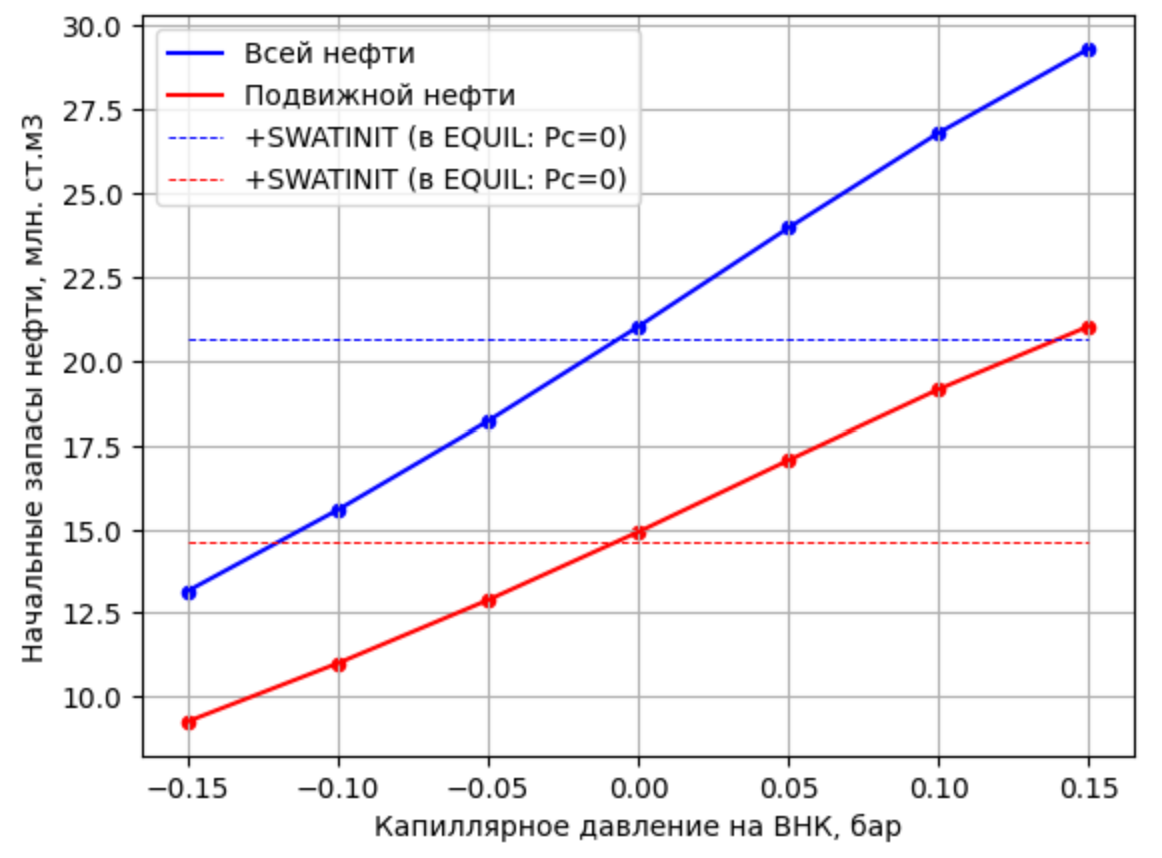
\includegraphics[width=.8\textwidth]{initial_reserves_plot}
\caption{График зависимости запасов нефти от капиллярного давления на ВНК}
\label{fig:initial_reserves_plot}
\end{figure}


\begin{figure}[H]
	\adjustbox{minipage=1.3em}{\subcaption{}\label{fig:saturation_1_model_1}}%
	\begin{subfigure}[t]{\dimexpr.5\linewidth-1.3em\relax}
		\centering
		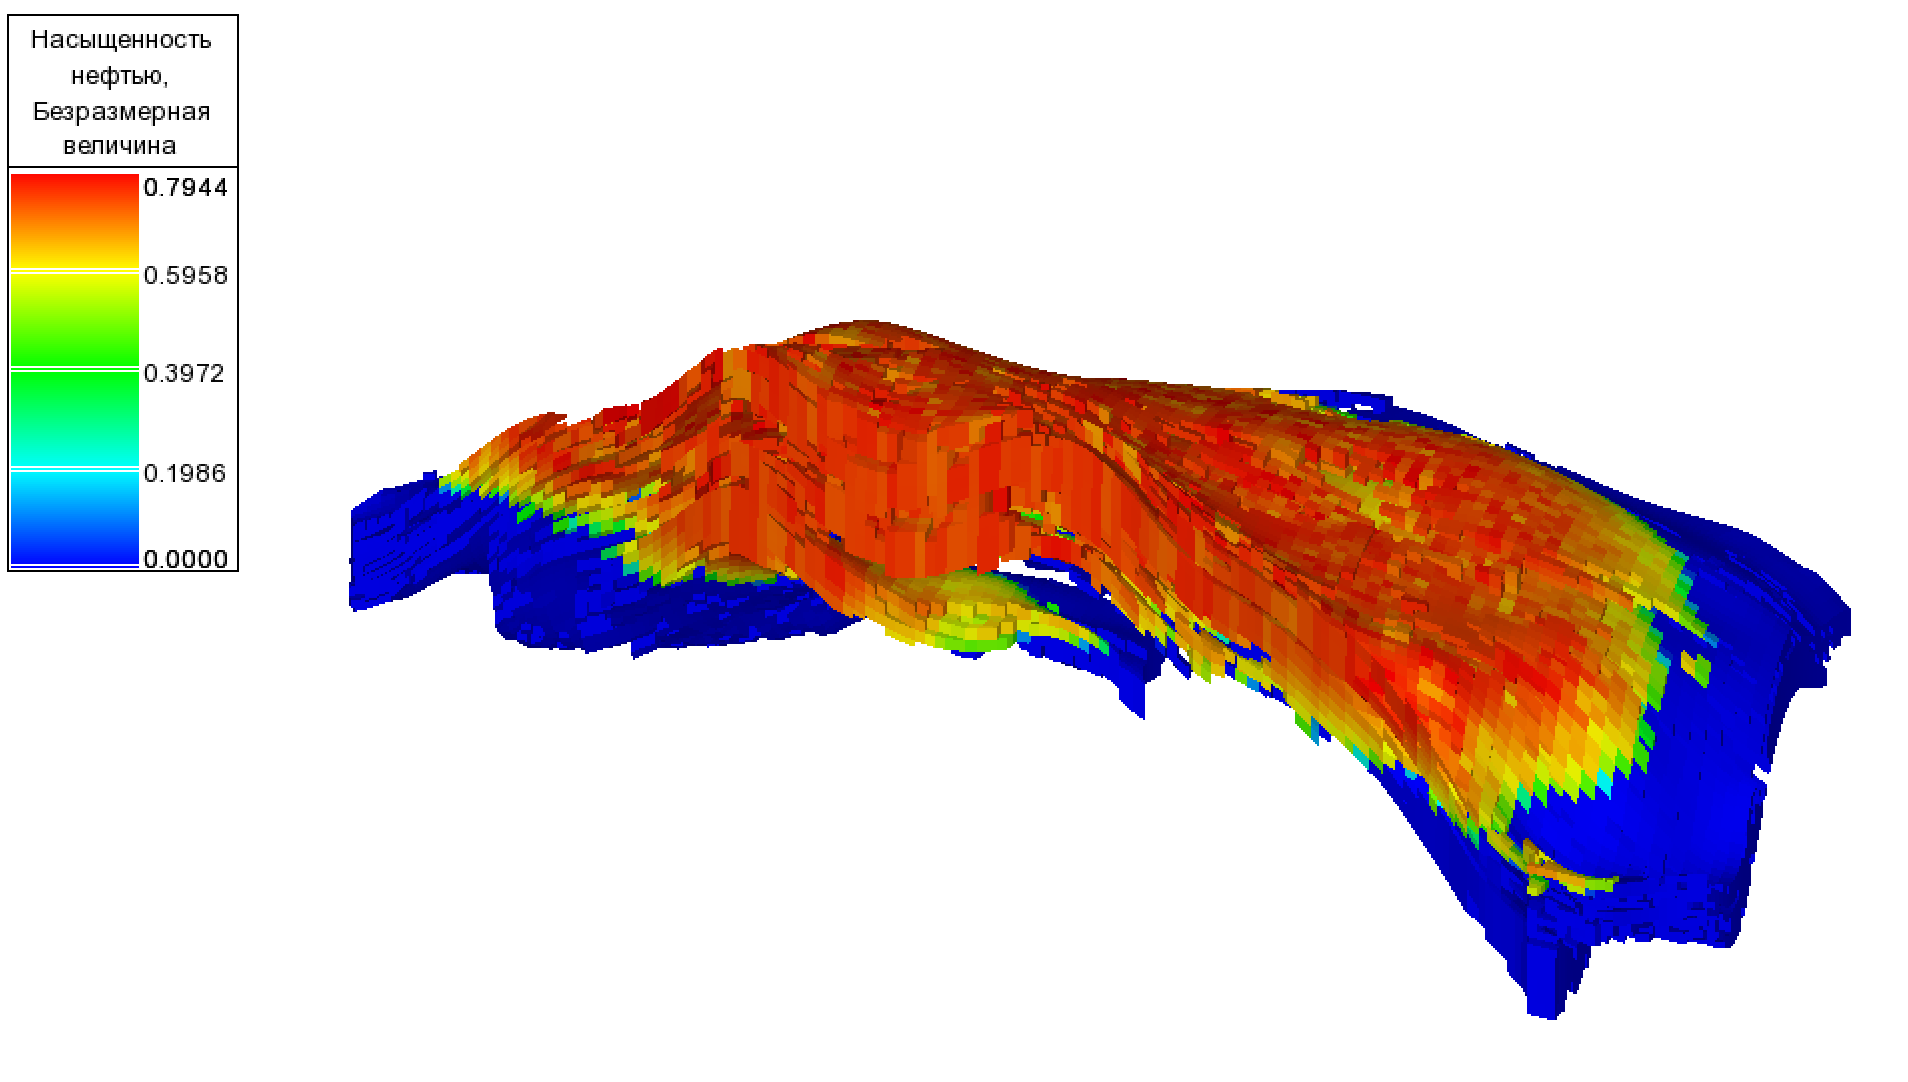
\includegraphics[width=.95\linewidth]{saturation_1_model_1}
	\end{subfigure}
\hfill %выровнять по ширине
	\adjustbox{minipage=1.3em}{\subcaption{}\label{fig:saturation_2_model_1}}%
	\begin{subfigure}[t]{\dimexpr.5\linewidth-1.3em\relax}
		\centering
		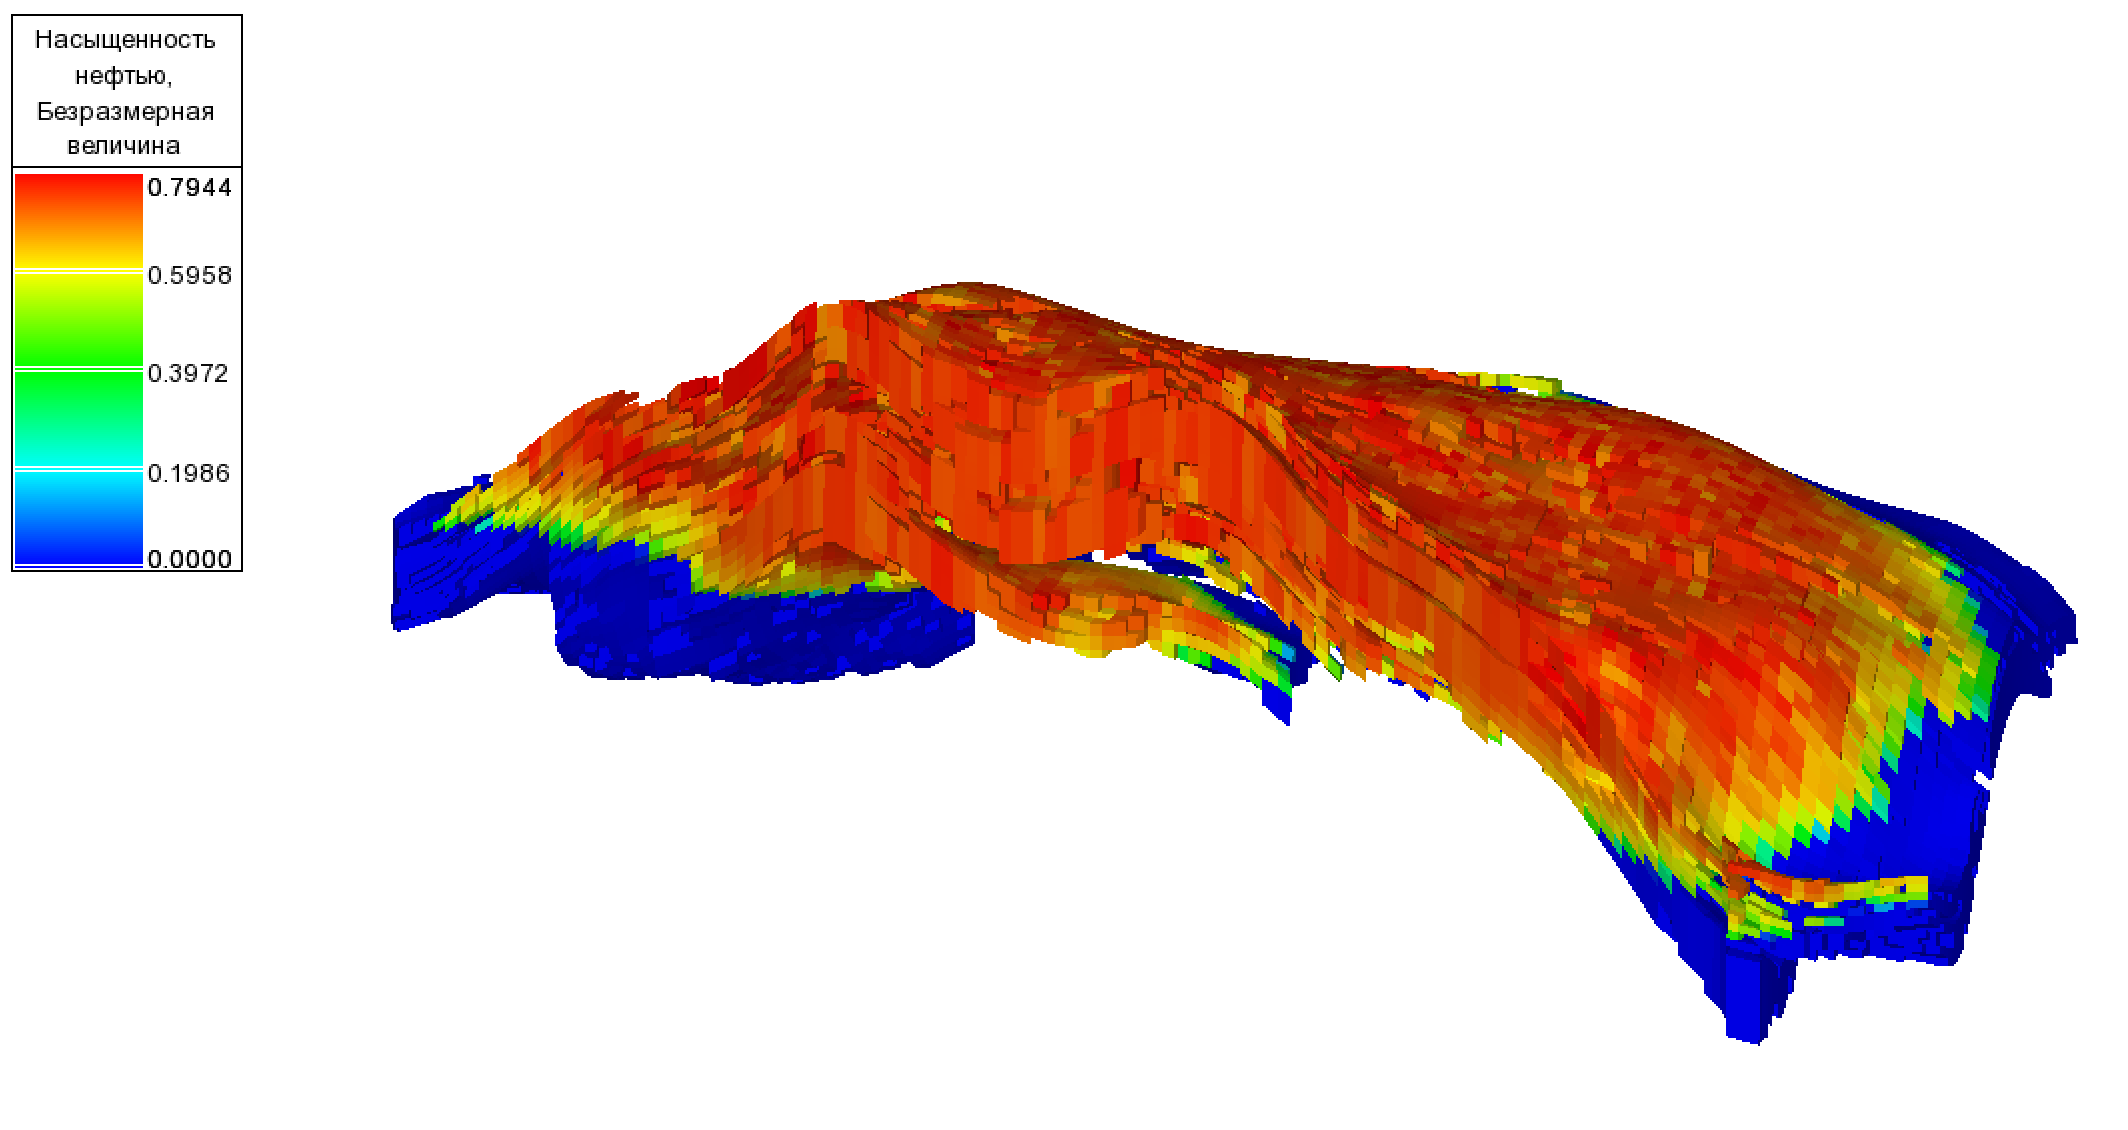
\includegraphics[width=.95\linewidth]{saturation_2_model_1}
	\end{subfigure}
\\[20pt]
	\adjustbox{minipage=1.3em}{\subcaption{}\label{fig:saturation_3_model_1}}%
\begin{subfigure}[t]{\dimexpr.5\linewidth-1.3em\relax}
	\centering
	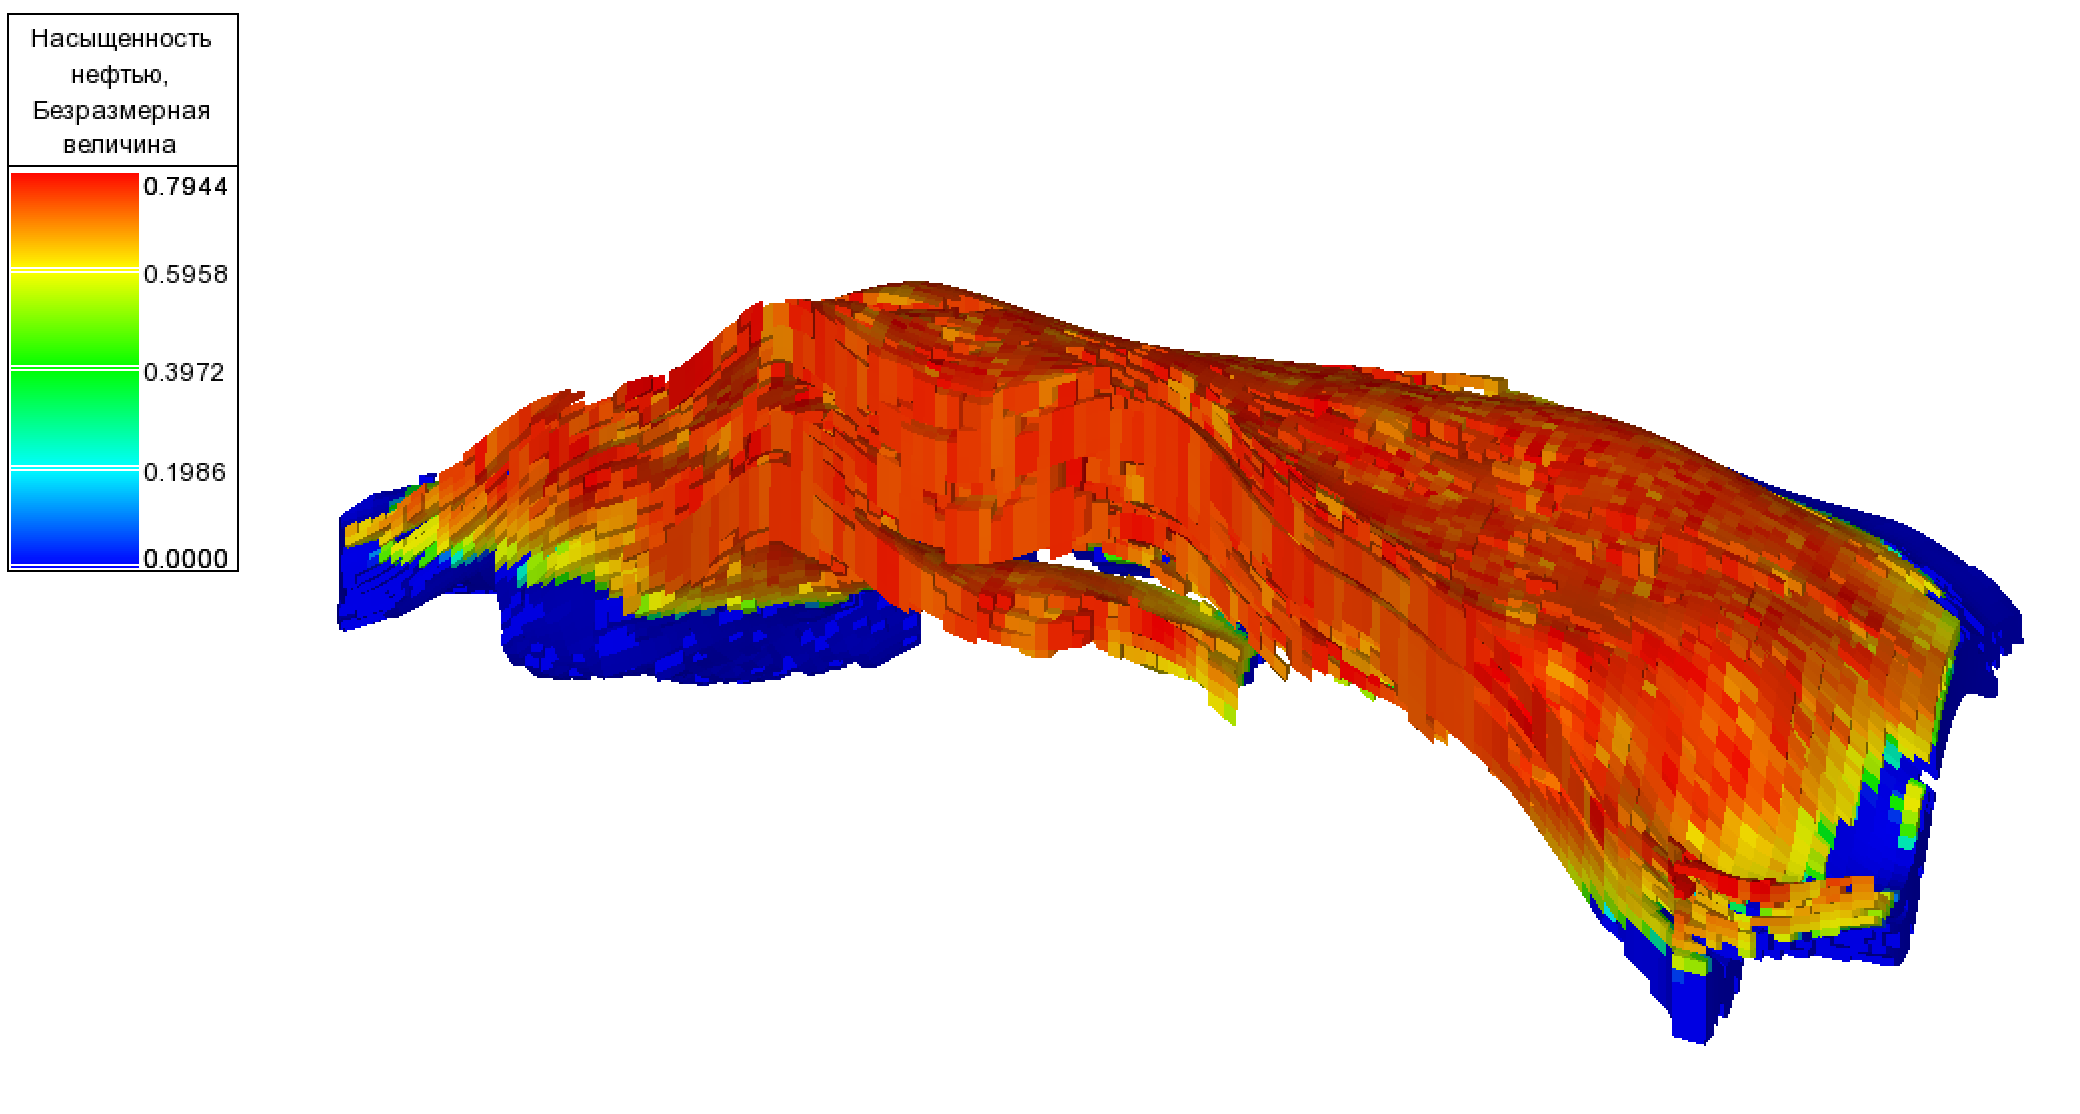
\includegraphics[width=.95\linewidth]{saturation_3_model_1}
\end{subfigure}%
\hfill %выровнять по ширине
\adjustbox{minipage=1.3em}{\subcaption{}\label{fig:saturation_4_model_1}}%
\begin{subfigure}[t]{\dimexpr.5\linewidth-1.3em\relax}
	\centering
	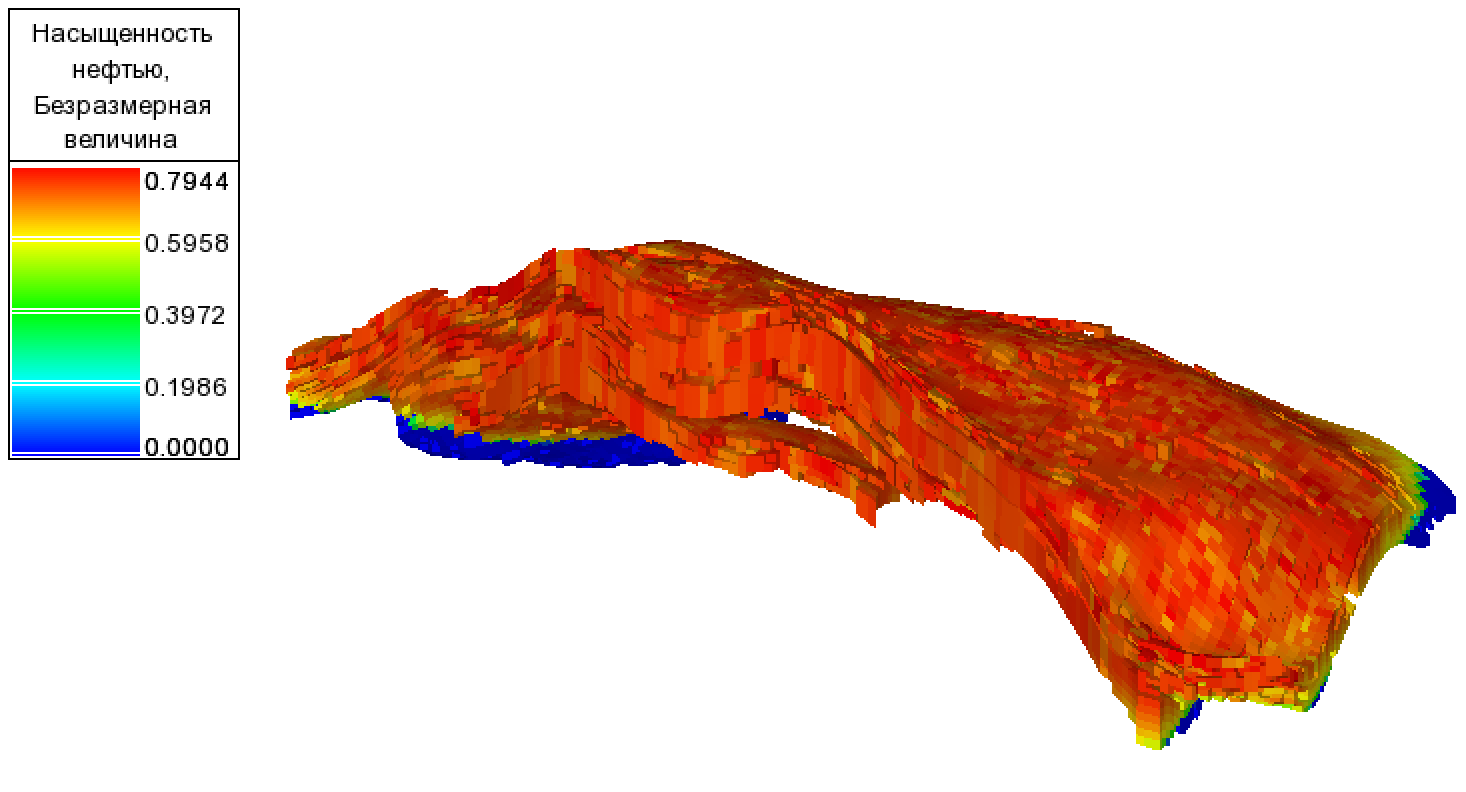
\includegraphics[width=.95\linewidth]{saturation_4_model_1}
\end{subfigure}
\captionsetup{justification=centering} %центрировать
\caption{Начальное распределение нефтенасыщенности: ({\itshape a}) $P_c=-0.1\text{ бар}$; ({\itshape b}) $P_c=0\text{ бар}$; \\({\itshape c}) $P_c=0.1\text{ бар}$; ({\itshape d}) $P_c=0.3\text{ бар}$} 
\label{fig:initial_saturation}
\end{figure}


\subsection{Инициализация EQUIL + SWATINIT}

Если необходимо строго соблюдать имеющиеся геологические запасы, то геолог передаёт нам куб водонасыщенности и мы его подключаем в модель с помощью ключевого слова SWATINIT.
При таком способе инициализации у симулятора получается две насыщенности: одну он сам рассчитал через условие равновесия, а другая задана в кубе SWATINIT.
Если они не совпали, симулятор будет масштабировать кривую капиллярного давления таким образом, чтобы насыщенность совпала со значениями в SWATINIT. 

В конце секции \textbf{PROPS} подключим файл SWATINIT.inc.
В этом файле с помощью ключевого слова SWATINIT указаны начальные водонасыщенности блоков сетки, которые должны быть получены симулятором с помощью масштабирования конечных точек фазовых проницаемостей.
Капиллярное давление воды будет масштабировано таким образом, чтобы водонасыщенности, рассчитанные с помощью фазового равновесия, совпали с указанными в данном ключевом слове.

\begin{eclrun}
INCLUDE
'INC\SWATINIT.inc' /
\end{eclrun}


\begin{figure}[H]
\center
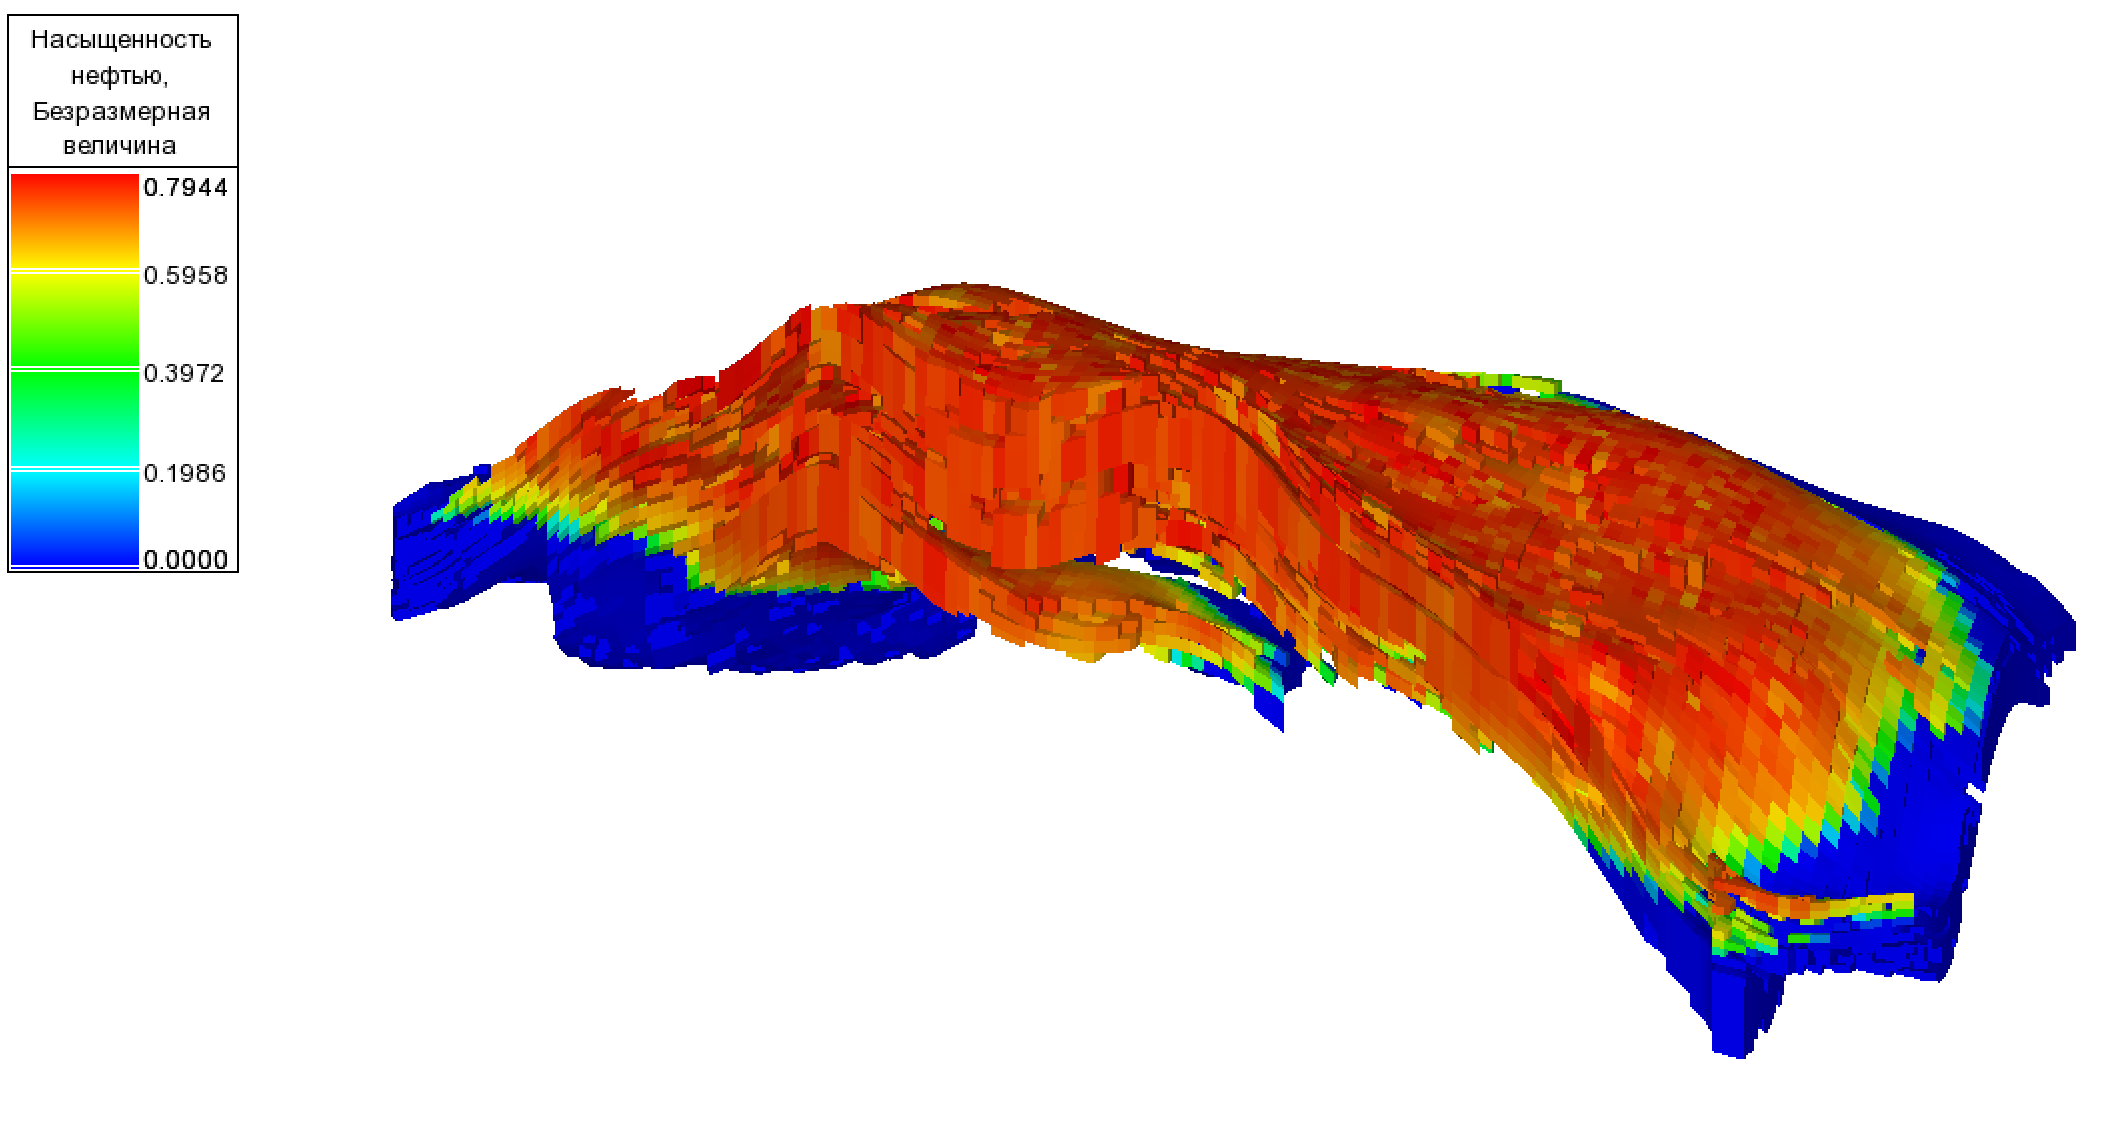
\includegraphics[width=\textwidth]{saturation_SWATINIT_model_1}
\caption{Начальное распределение нефтенасыщенности при $P_c=0$ бар и заданным кубом водонасыщенности SWATINIT -- визуализация tNavigator}
\label{fig:saturation_SWATINIT_model_1}
\end{figure}

\newpage
\section{Задание от 19.10.2022}

Собрать секцию SCHEDULE на основе подготовленных данных по траекториям скважин, перфорациям, замерам давления, добыче, распределению скважин по группам и модели из задания от 05.10.2022.

\subsection{Использование ключевого слова ARITHMETIC}

Ключевое слово ARITHMETIC доступно в т-Навигаторе, но не работает в Eclipse-е.
Позволяет более элегантно задать зависимости проницаемости и концевых точек ОФП от пористости.
Но по сути полностью равносильно действию ключевого слова OPERATE из модели от 05.10.2022.

В секции \textbf{GRID}:
\begin{eclrun}
ARITHMETIC
PERMX=14593.4635*((MAX(PORO,0.00001))^2.62189)
PERMY=PERMX
PERMZ=0.499*PERMX
/
\end{eclrun}

В секции \textbf{PROPS}:
\begin{eclrun}
ARITHMETIC
SWCR=-0.04705*LOG(PERMX)+0.52721
SOWCR=-0.01289*LOG(PERMX)+0.27396
KRWR=0.06701*LOG(PERMX)-0.14287
SWU=1
KRORW=0.833
KRO=1
KRW=1
SWL=SWCR
/
\end{eclrun}

\subsection{Секция SCHEDULE}
Секция \textbf{SCHEDULE} собрана в т-Навигаторе с помощью опции Загрузить данные по скважинам.

Дополнительно можем собрать секцию \textbf{SCHEDULE} в ПО SCHEDULE (поставляемом вместе с Eclipse-ом) и подключить её к data-файлу с моделью (в секции \textbf{SCHEDULE}):
\begin{eclrun}
INCLUDE
'INC\SCHEDULE.SCH' /
\end{eclrun}

При таком подходе в рассматриваемом примере результат совпадает с результатом в т-Навигаторе.


\begin{figure}[H]
\center
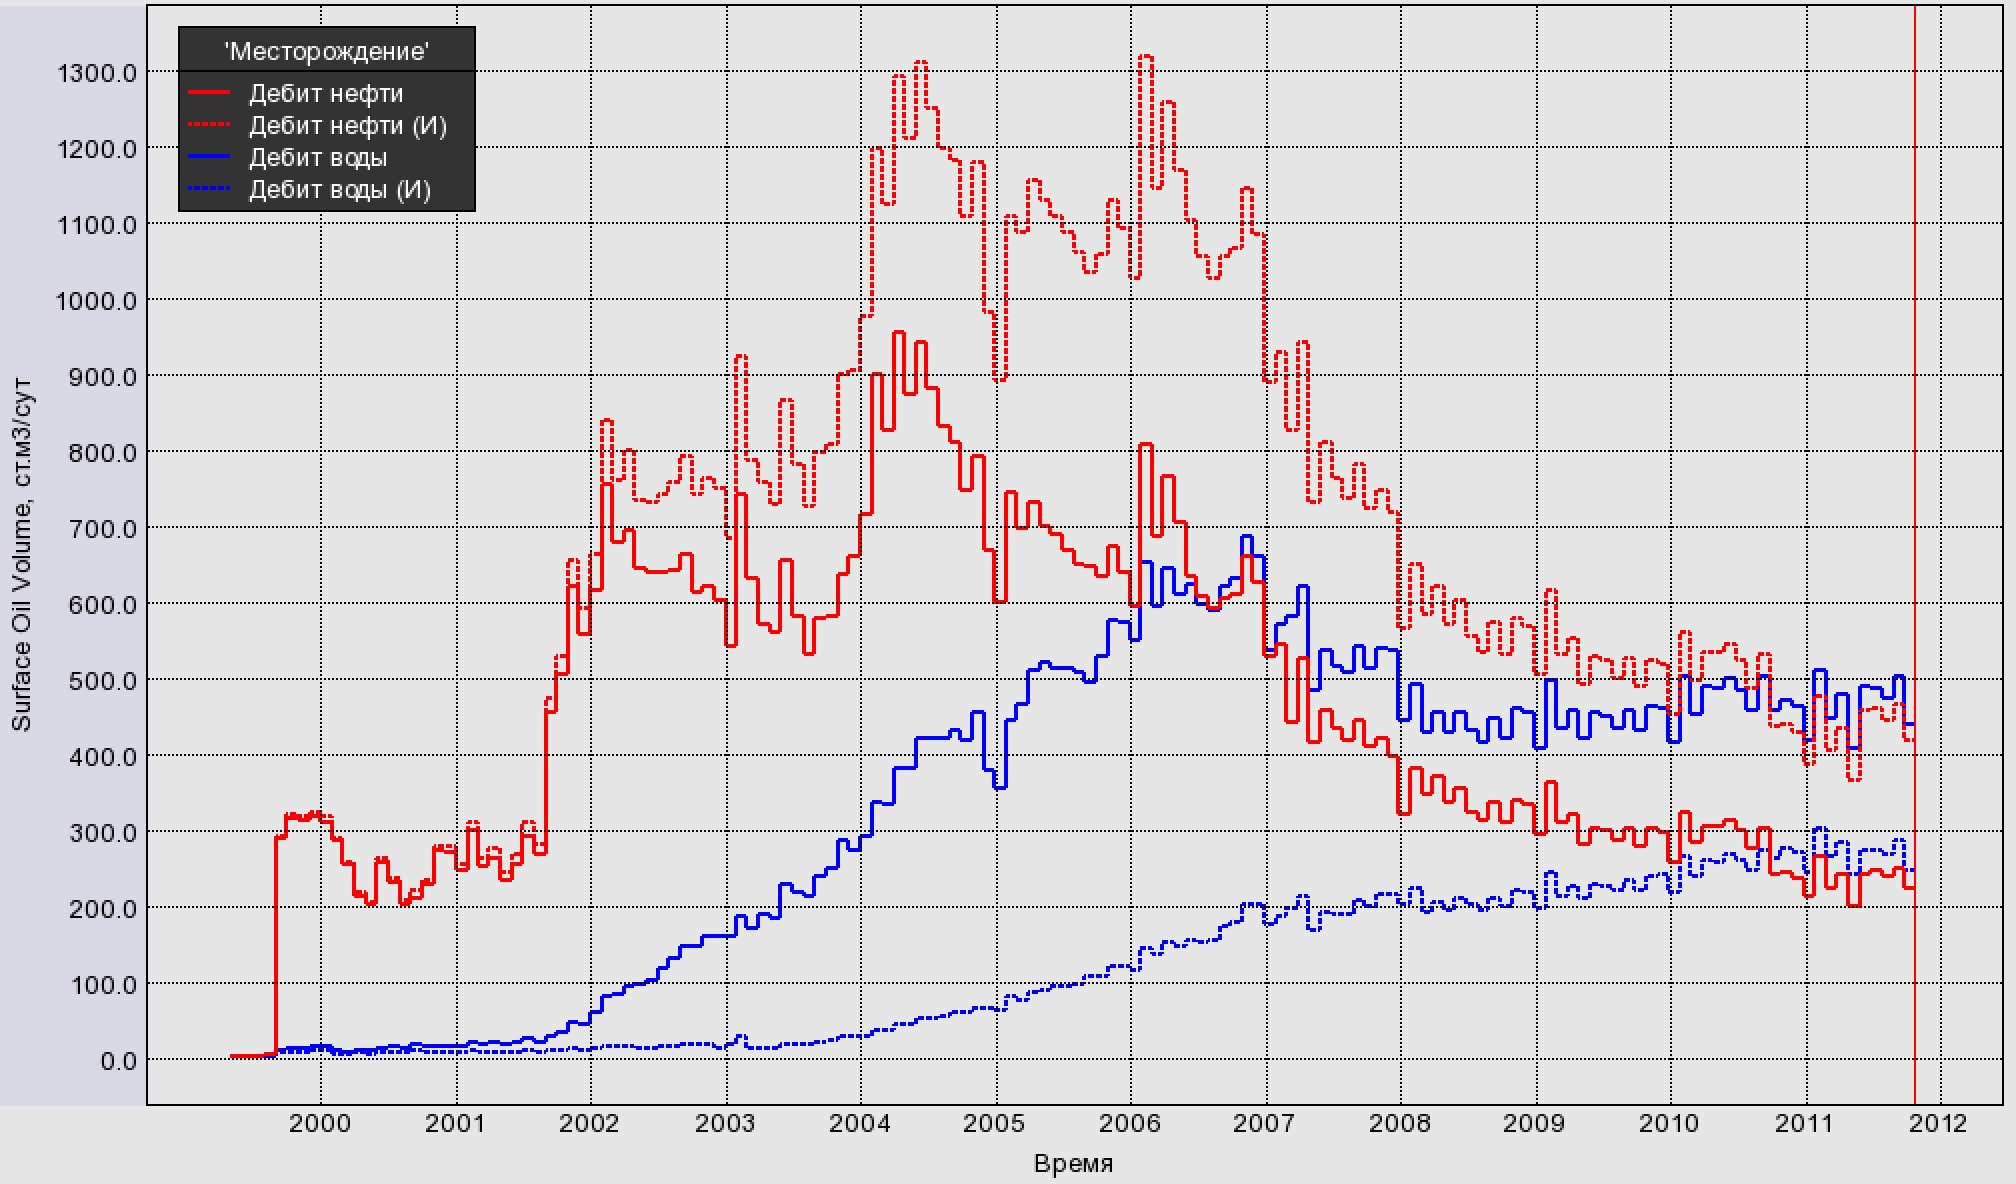
\includegraphics[width=\textwidth]{rates_model_schedule}
\caption{Фактические (исторические) и рассчитанные графики дебитов нефти и воды (суммарно со всех скважин по месторождению) для исходной модели}
\label{fig:history_and_calculate}
\end{figure}

Из рис. \ref{fig:history_and_calculate} видим, что для исходной модели адаптация не проводилась: рассчитанные значения дебитов нефти существенно занижены, а рассчитанные значения дебитов воды завышены относительно фактических (исторических) значений.

\newpage
\section{Задание от 26.10.2022}

\subsection{Расчёт моделей с разными наборами исходных данных}

Получаемый при моделировании результат чувствителен к исходным данным.
Требуется проверить, как изменится расчёт при отсутствии или некорректности некоторых данных:

\begin{itemize}
	\item нет исследования анизотропии проницаемости. Расчёт с анизотропией 0.1
	\item в наличии только одно исследование ОФП. Расчёт с ОФП Sample 4
	\item взятая ранее для расчётов проба оказалась некондиционной (частично разгазированной). Новая уточнённая глубинная проба нефти:
	$$\rho_{\text{oil}}=836\,\frac{\text{кг}}{\text{м}^3}
	\,\,\,\,\,\,\,C_0=1.46\cdot10^{-4}\,\text{бар}^{-1}
	\,\,\,\,\,\,\,P_b=58\,\text{бар}$$
	$$R_s=40\,\frac{\text{м}^3}{\text{м}^3}
	\,\,\,\,\,\,\,B_o\!\left(P_b\right)=1.18\,\frac{\text{м}^3}{\text{м}^3}
	\,\,\,\,\,\,\,\mu_{\text{oil}}=5.2\,\text{мПа}\cdot\text{с}$$
\end{itemize}

Результат расчёта моделей с разными наборами исходных данных представлен на рис. \ref{fig:rates_variations} и рис. \ref{fig:nakop_variations}.

\begin{figure}[H]
	\adjustbox{minipage=1.3em}{\subcaption{}\label{fig:rates_variations_1}}%
	\begin{subfigure}[t]{\dimexpr.5\linewidth-1.3em\relax}
		\centering
		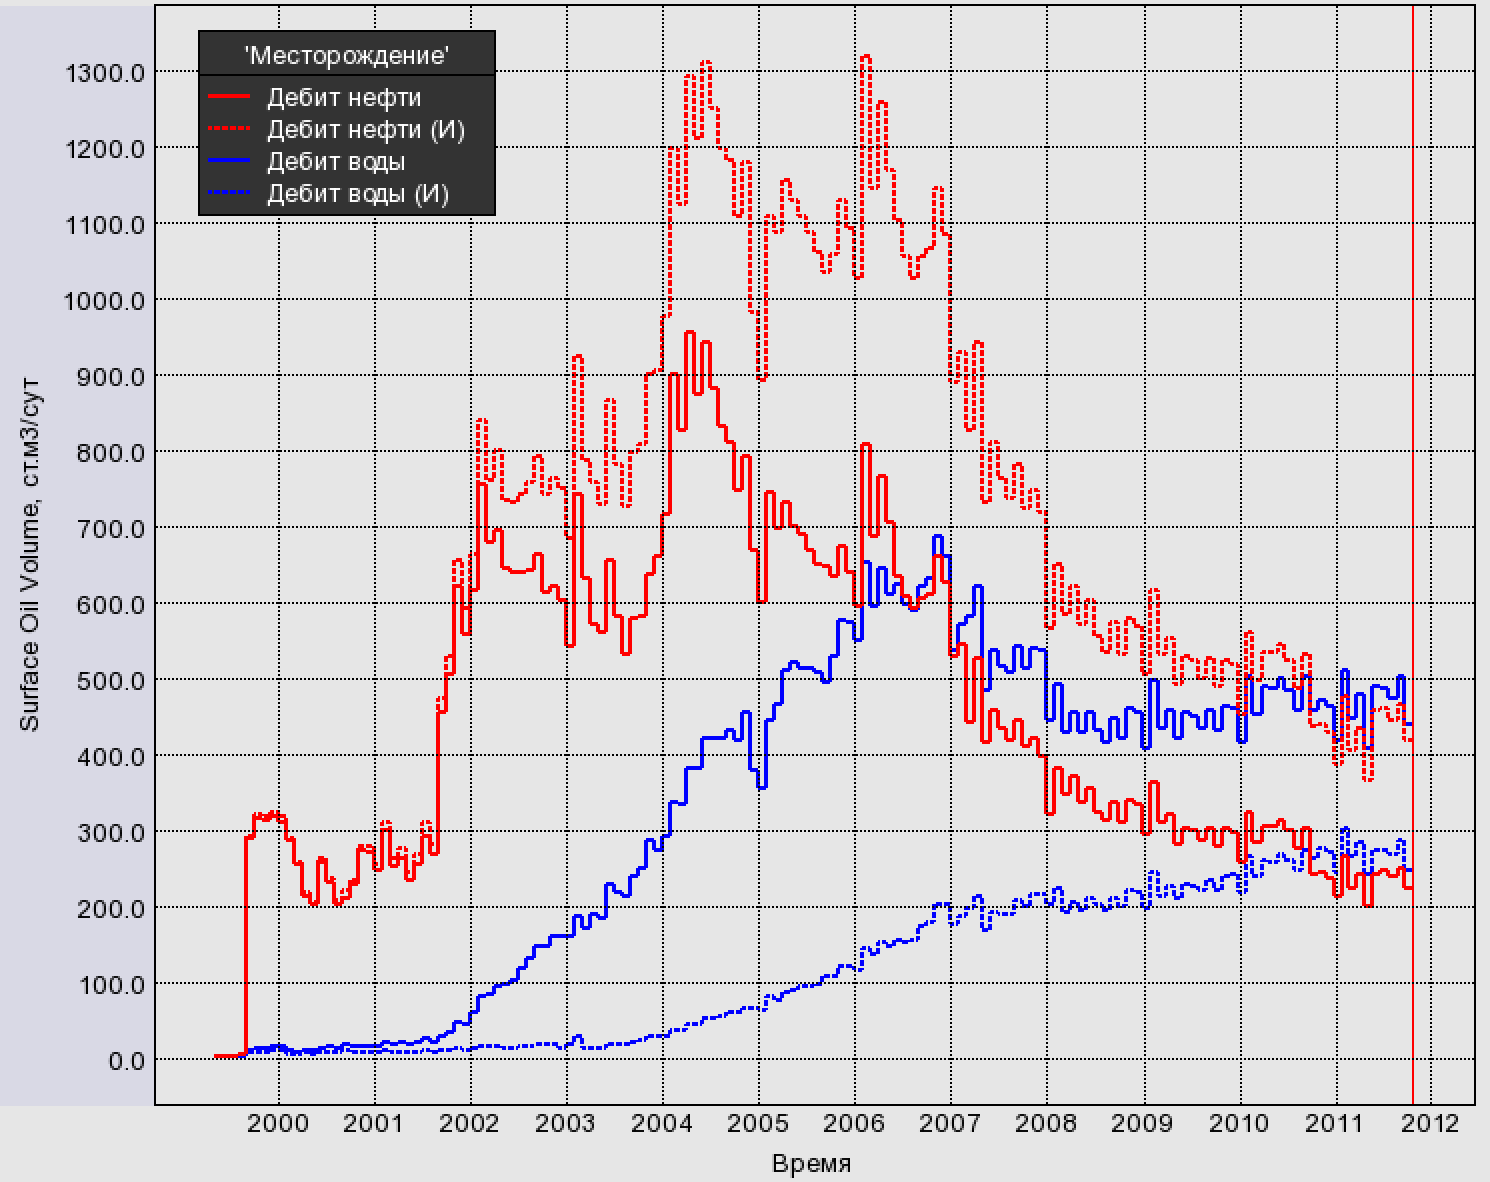
\includegraphics[width=.9\linewidth]{rates_default_model}
	\end{subfigure}
\hfill %выровнять по ширине
	\adjustbox{minipage=1.3em}{\subcaption{}\label{fig:rates_variations_2}}%
	\begin{subfigure}[t]{\dimexpr.5\linewidth-1.3em\relax}
		\centering
		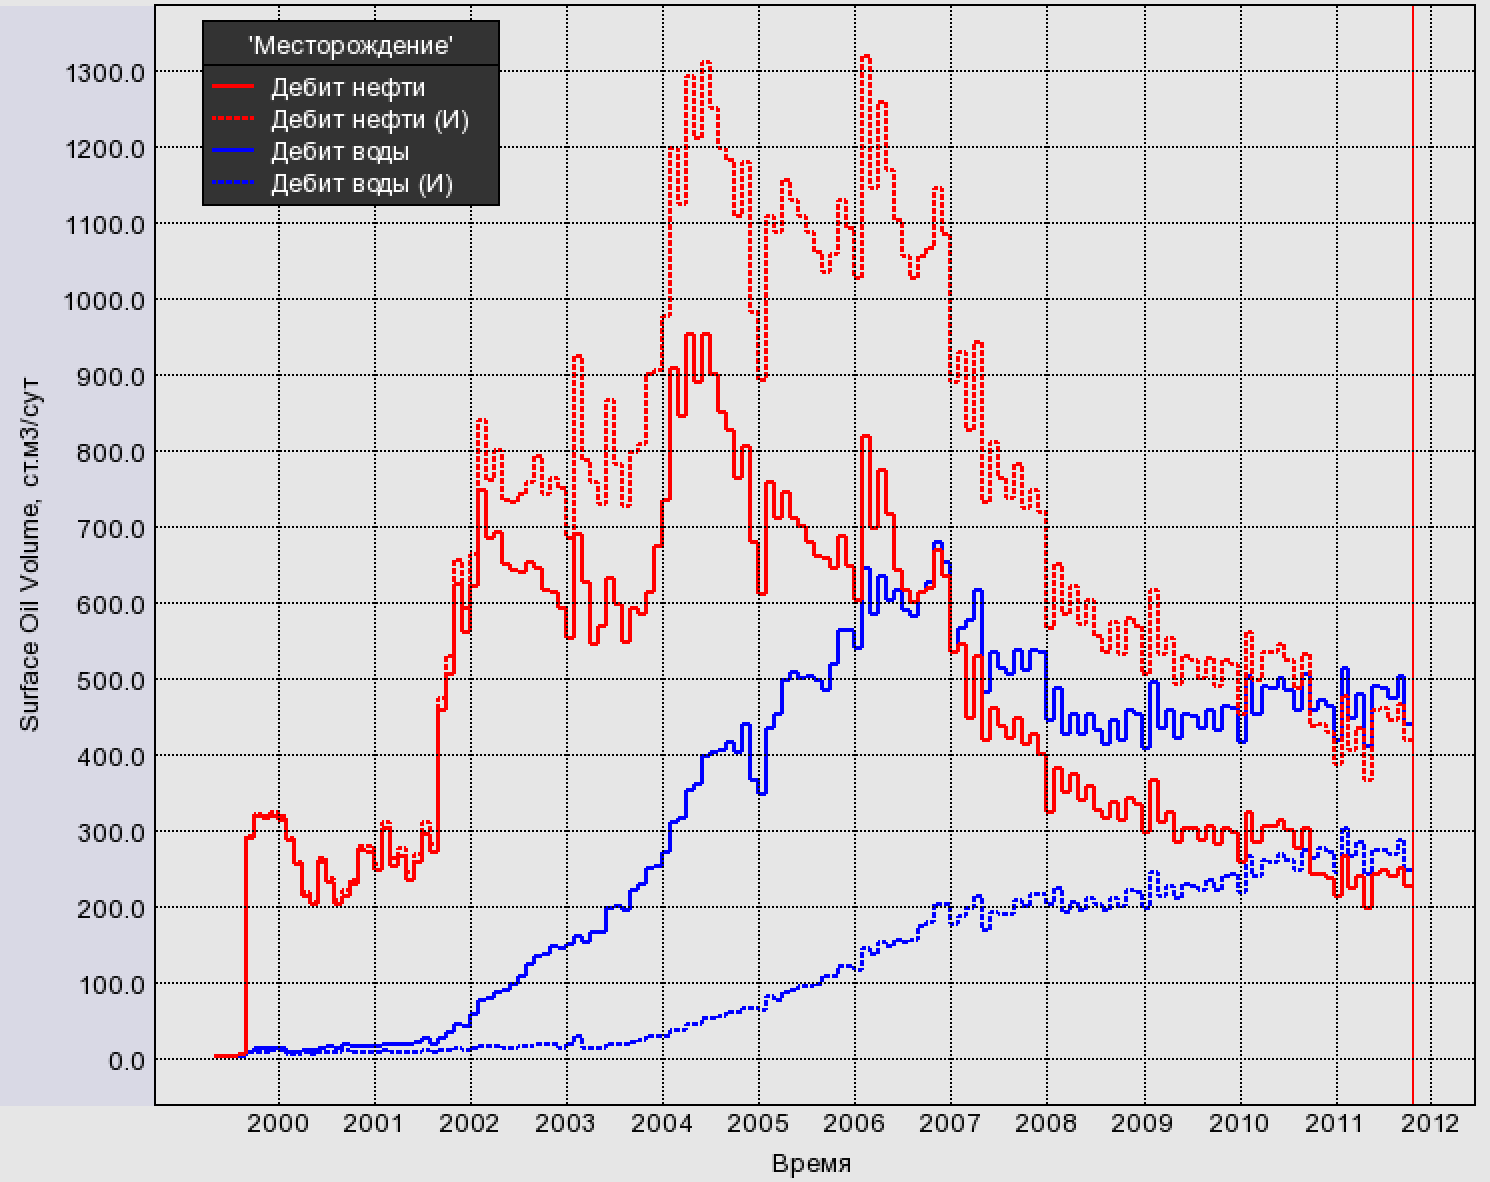
\includegraphics[width=.9\linewidth]{rates_anizotropy_model}
	\end{subfigure}
\\[20pt]
	\adjustbox{minipage=1.3em}{\subcaption{}\label{fig:rates_variations_3}}%
\begin{subfigure}[t]{\dimexpr.5\linewidth-1.3em\relax}
	\centering
	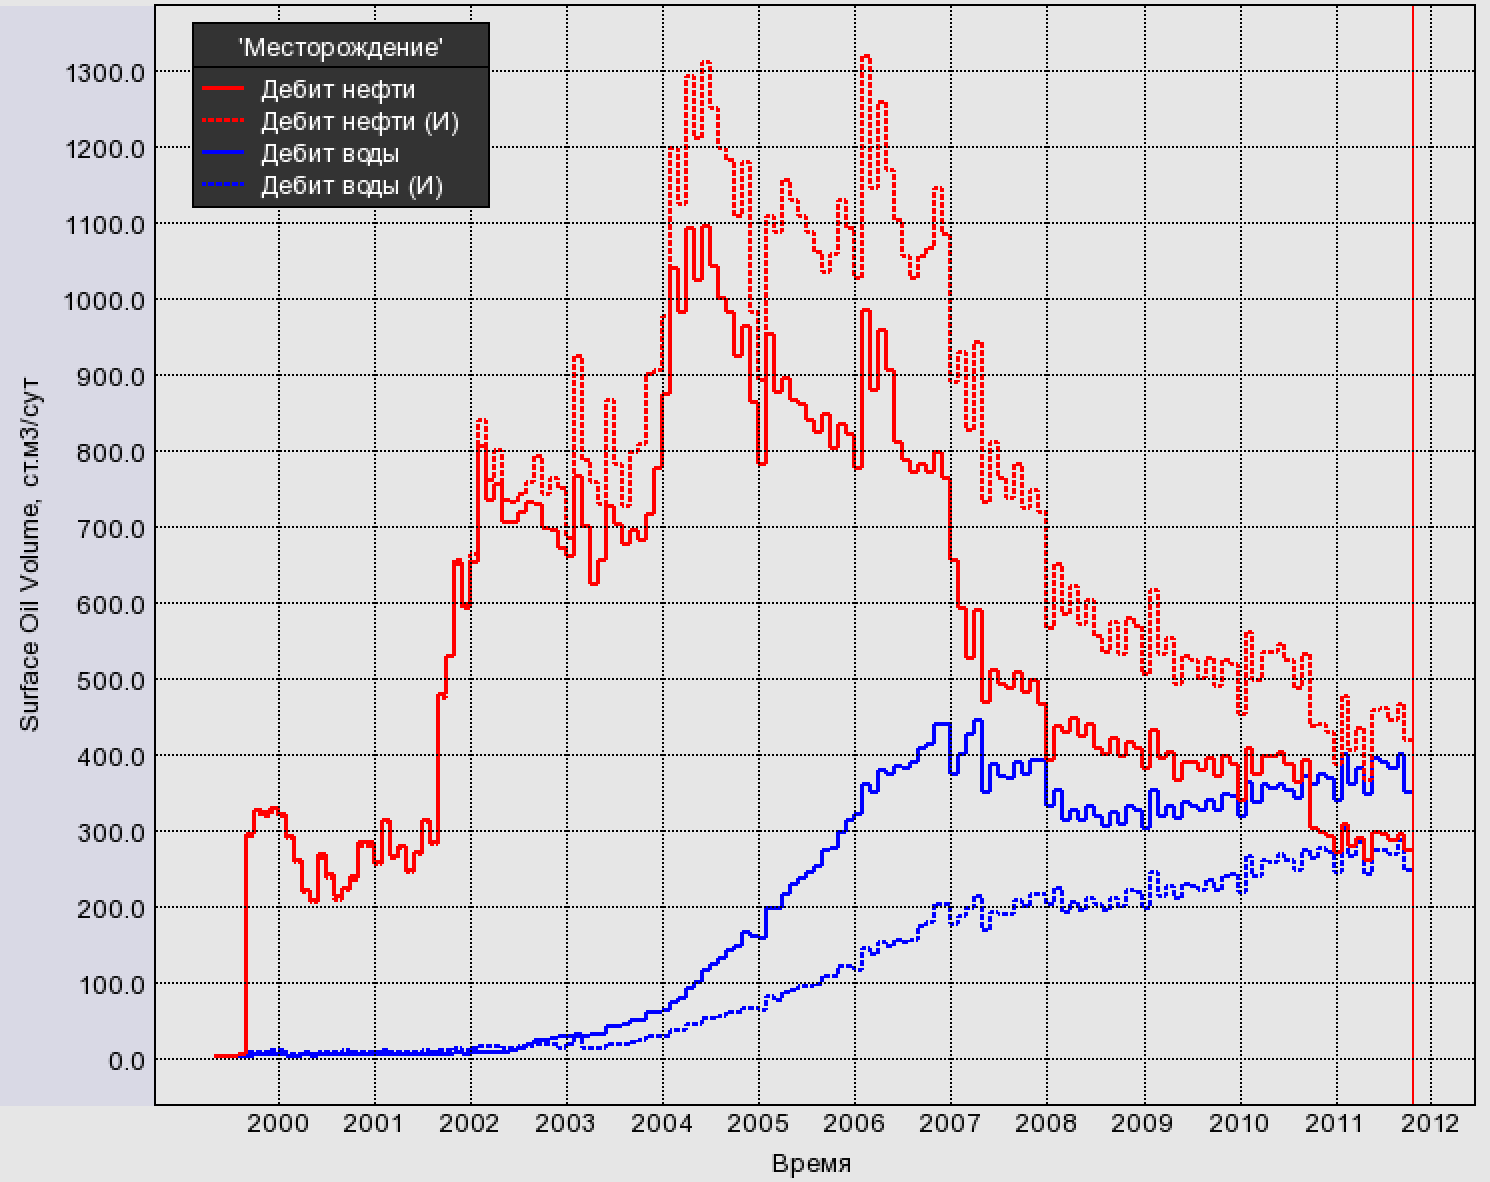
\includegraphics[width=.9\linewidth]{rates_ofp_model}
\end{subfigure}%
\hfill %выровнять по ширине
\adjustbox{minipage=1.3em}{\subcaption{}\label{fig:rates_variations_4}}%
\begin{subfigure}[t]{\dimexpr.5\linewidth-1.3em\relax}
	\centering
	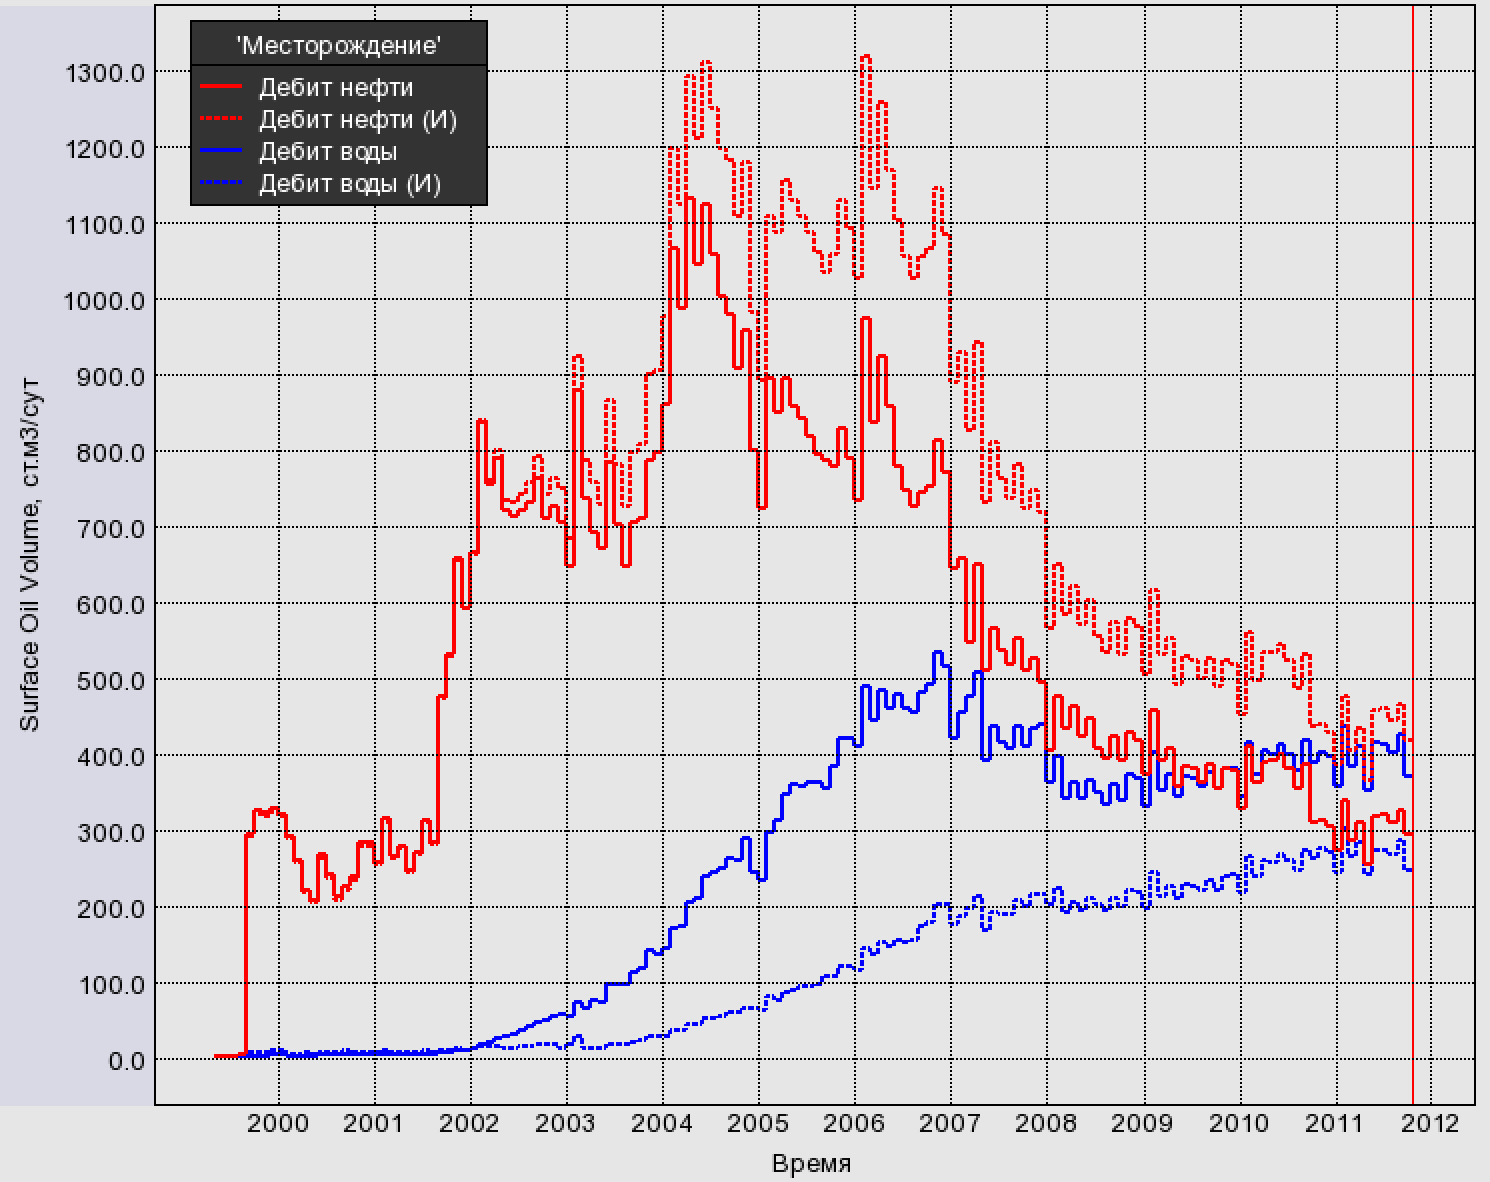
\includegraphics[width=.9\linewidth]{rates_pvt_model}
\end{subfigure}
\captionsetup{justification=centering} %центрировать
\caption{Графики зависимости дебитов нефти и воды от времени: ({\itshape a}) исходная модель; ({\itshape b}) с анизотропией 0.1; ({\itshape c}) с ОФП Sample 4; ({\itshape d}) с уточнёнными PVT-свойствами} 
\label{fig:rates_variations}
\end{figure}


\begin{figure}[H]
	\adjustbox{minipage=1.3em}{\subcaption{}\label{fig:nakop_variations_1}}%
	\begin{subfigure}[t]{\dimexpr.5\linewidth-1.3em\relax}
		\centering
		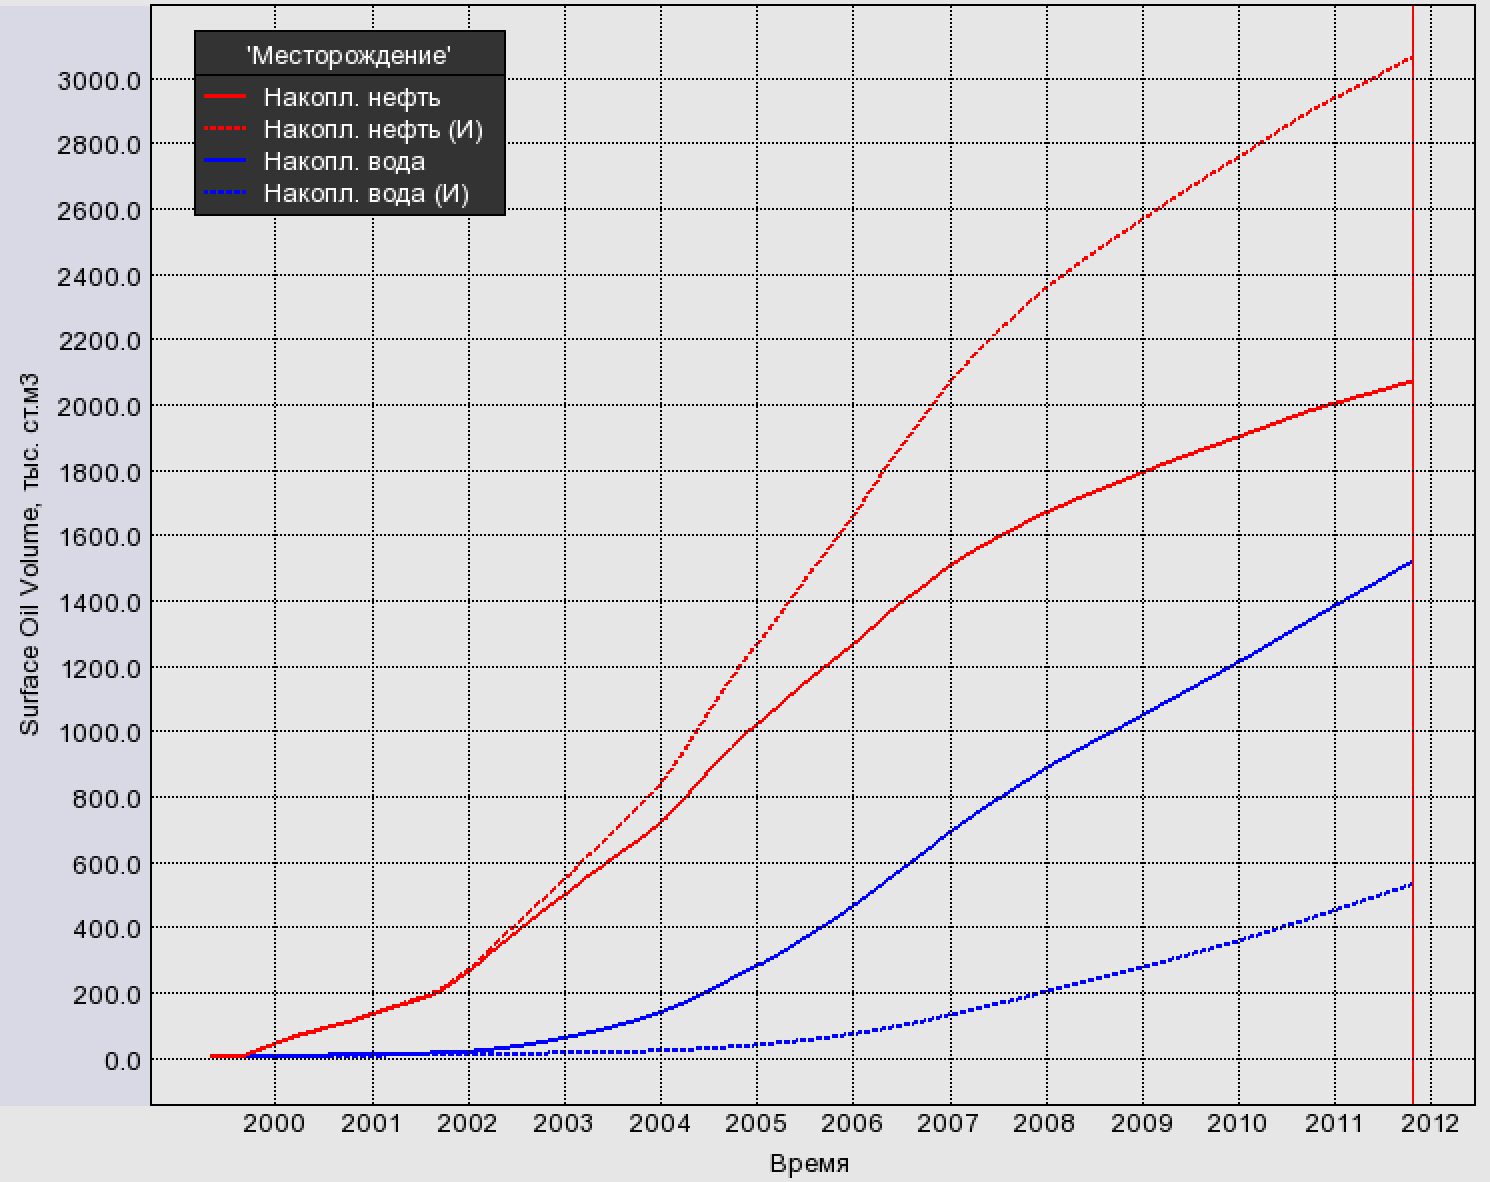
\includegraphics[width=.95\linewidth]{nakop_default_model}
	\end{subfigure}
\hfill %выровнять по ширине
	\adjustbox{minipage=1.3em}{\subcaption{}\label{fig:nakop_variations_2}}%
	\begin{subfigure}[t]{\dimexpr.5\linewidth-1.3em\relax}
		\centering
		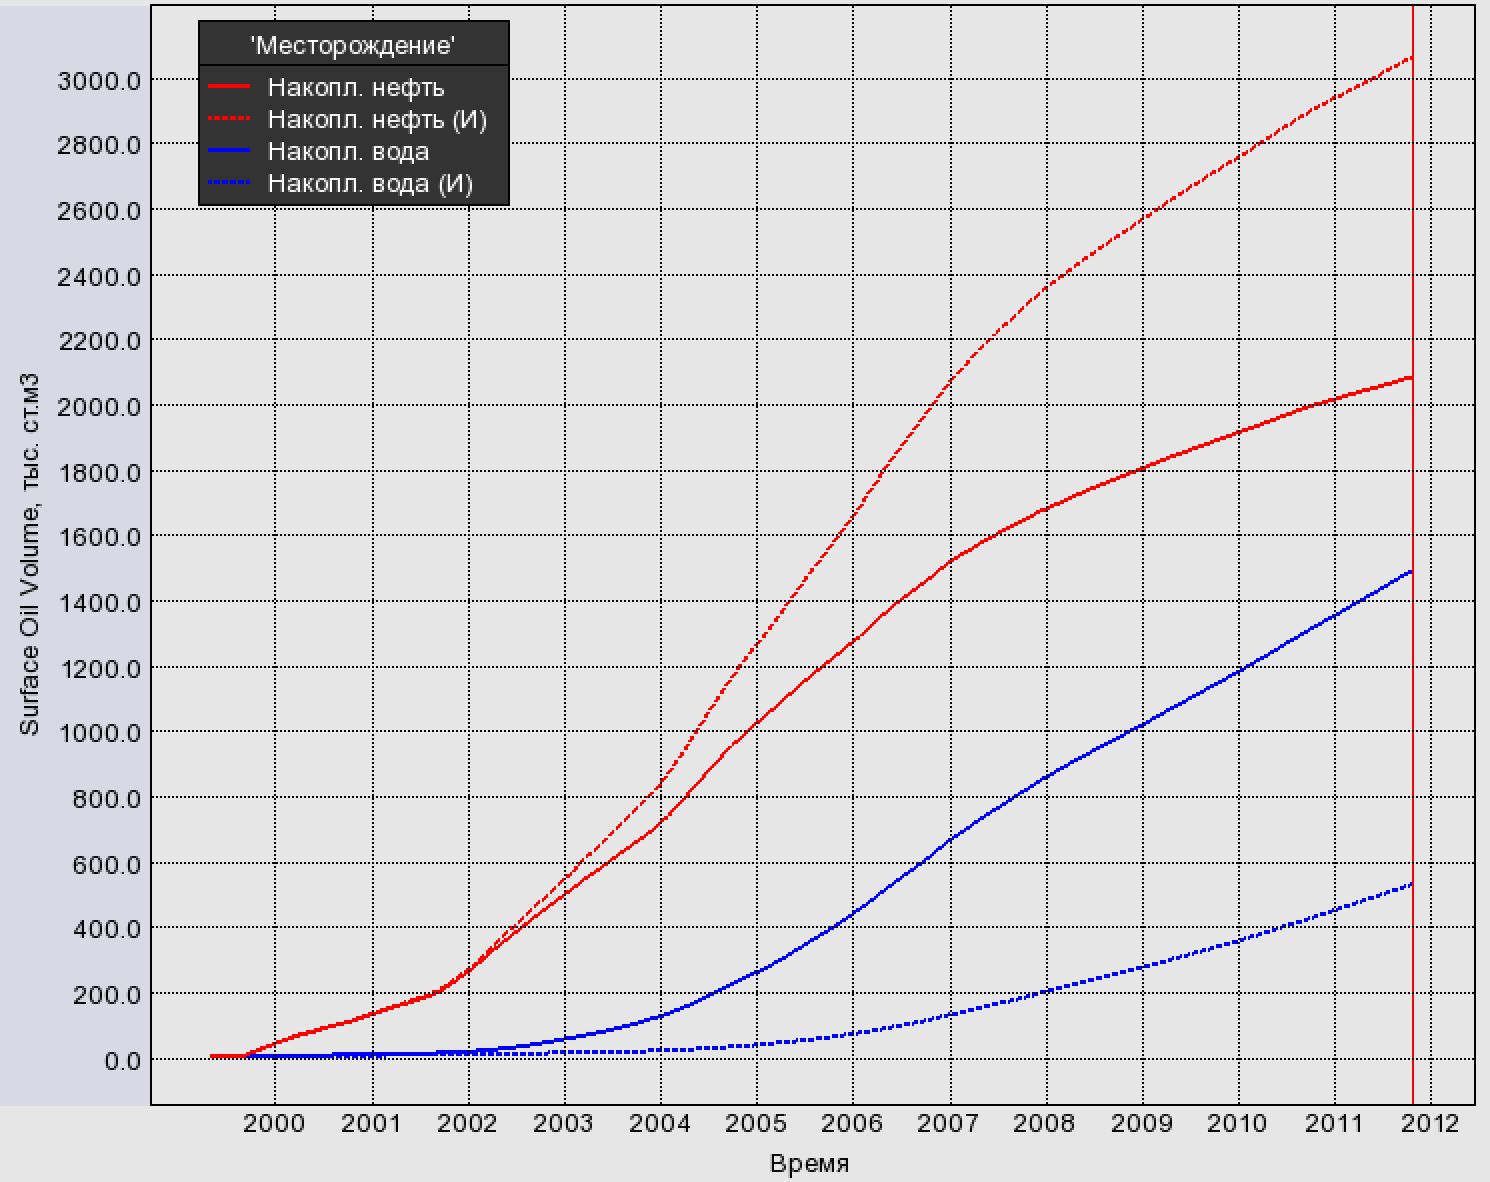
\includegraphics[width=.95\linewidth]{nakop_anizotropy_model}
	\end{subfigure}
\\[20pt]
	\adjustbox{minipage=1.3em}{\subcaption{}\label{fig:nakop_variations_3}}%
\begin{subfigure}[t]{\dimexpr.5\linewidth-1.3em\relax}
	\centering
	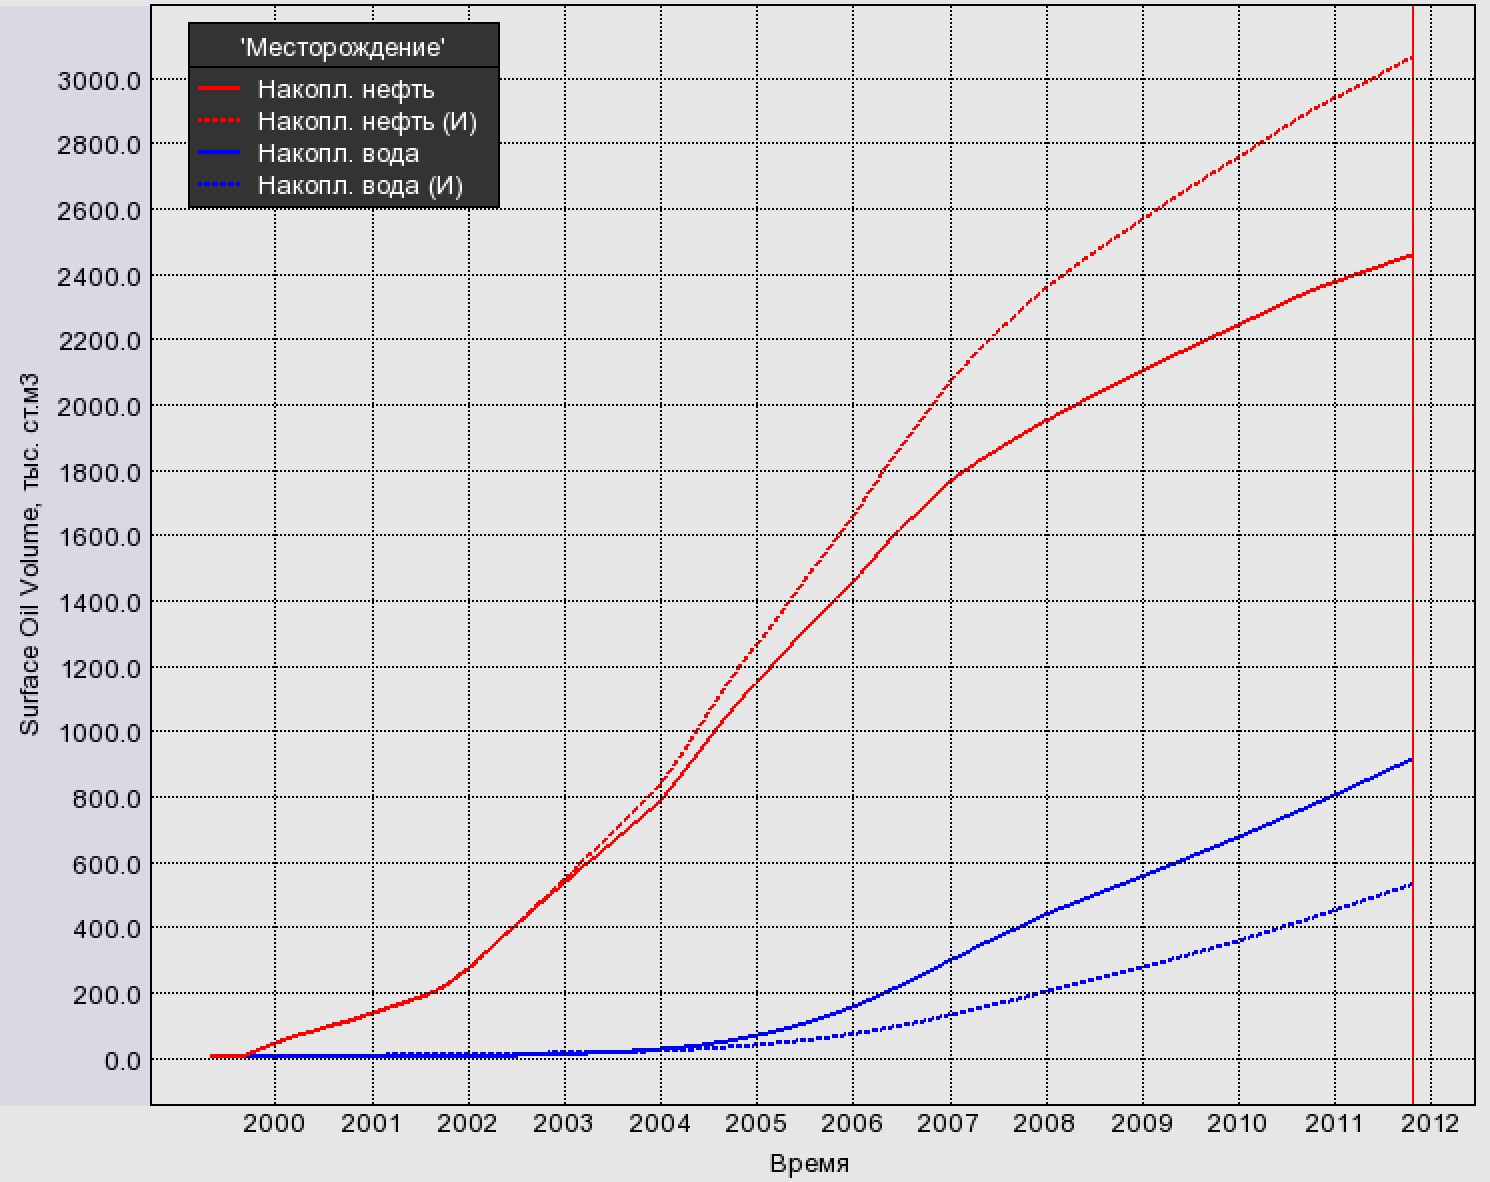
\includegraphics[width=.95\linewidth]{nakop_ofp_model}
\end{subfigure}%
\hfill %выровнять по ширине
\adjustbox{minipage=1.3em}{\subcaption{}\label{fig:nakop_variations_4}}%
\begin{subfigure}[t]{\dimexpr.5\linewidth-1.3em\relax}
	\centering
	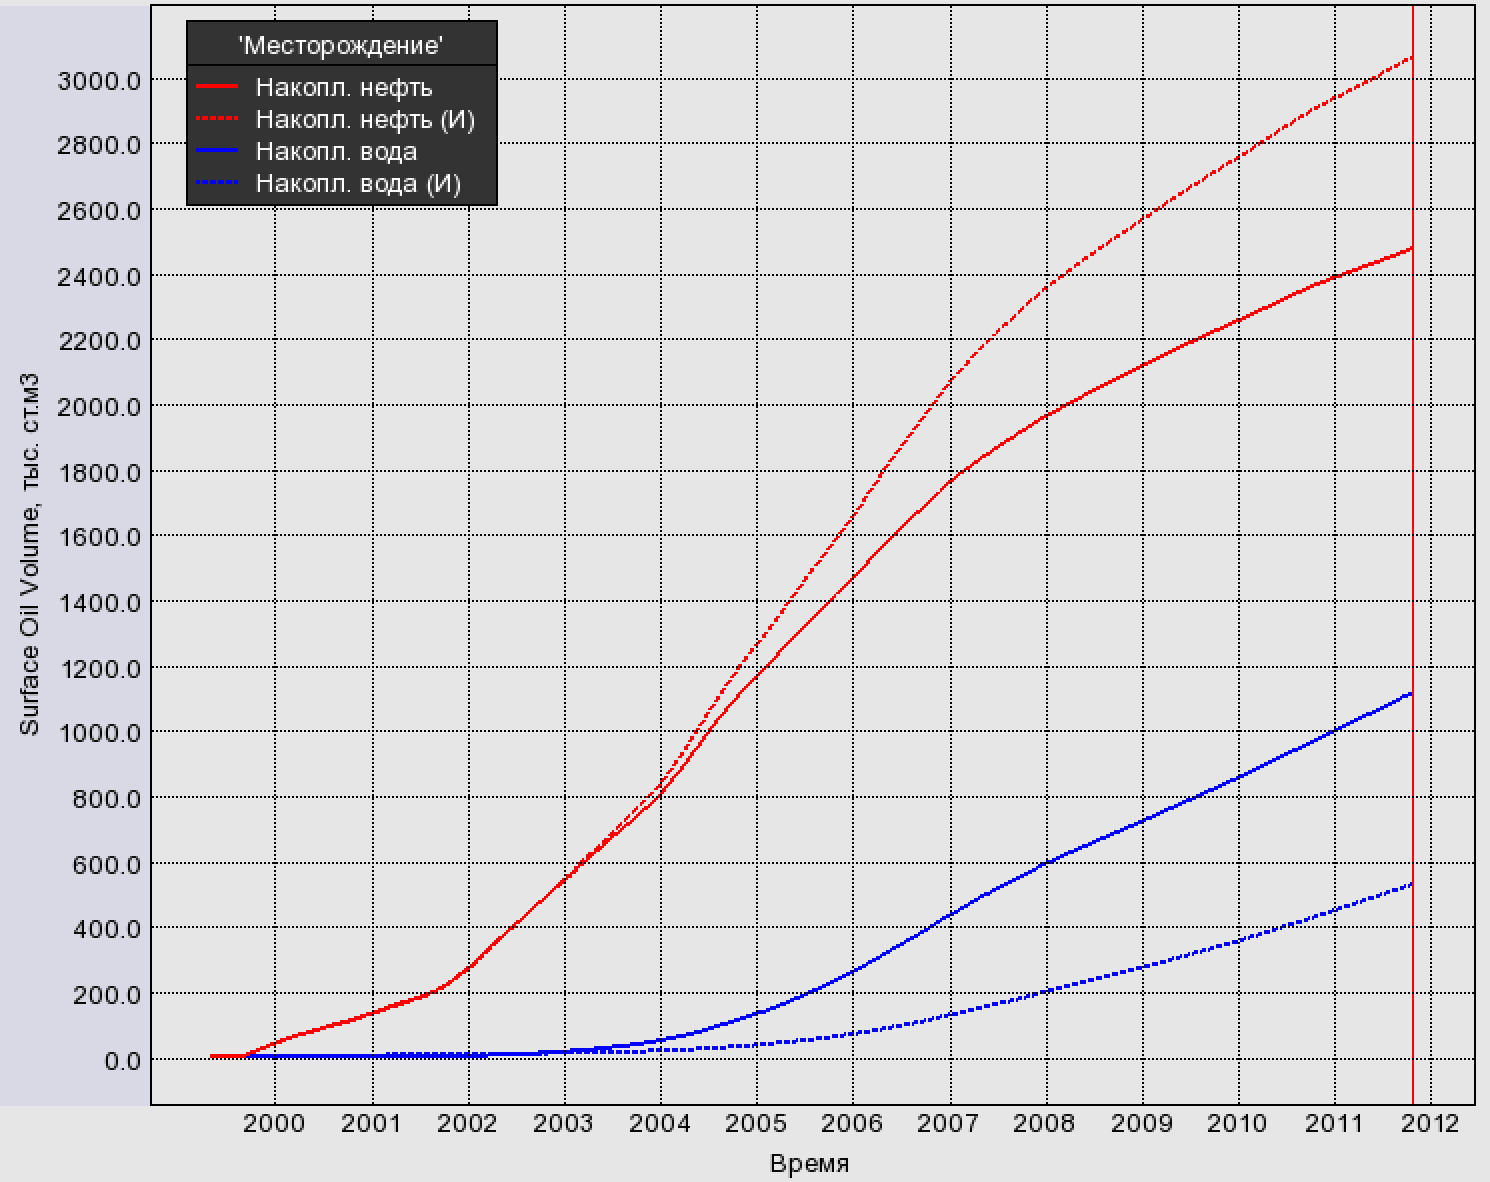
\includegraphics[width=.95\linewidth]{nakop_pvt_model}
\end{subfigure}
\captionsetup{justification=centering} %центрировать
\caption{Графики зависимости накопленной нефти и воды от времени: ({\itshape a}) исходная модель; ({\itshape b}) с анизотропией 0.1; ({\itshape c}) с ОФП Sample 4; ({\itshape d}) с уточнёнными PVT-свойствами} 
\label{fig:nakop_variations}
\end{figure}

Из полученных графиков видим, что отсутствие исследования анизотропии проницаемости (расчёт с анизотропией 0.1) совсем слабо повлияло на результат (а именно, на дебиты и накопленную добычу нефти и воды).

Изменение таблицы ОФП для системы вода-нефть существенно повлияло на итоговые результаты.
При этом рассчитанные результаты (суммарно по всему месторождению) стали ближе к историческим данным.

Уточнение PVT-свойств нефти тоже существенно повлияло на результат расчёта.

Из проведённых экспериментов с разными наборами исходных данных замечаем, что для адаптации модели разумно попытаться варьировать параметры ОФП и PVT-свойства.
\newpage

\subsection{Адаптация ГДМ}

Требуется:

\begin{itemize}
	\item просчитать модель, определить основные невязки
	\item варьируя различные параметры, садаптировать модель
\end{itemize}

\begin{figure}[H]
\center
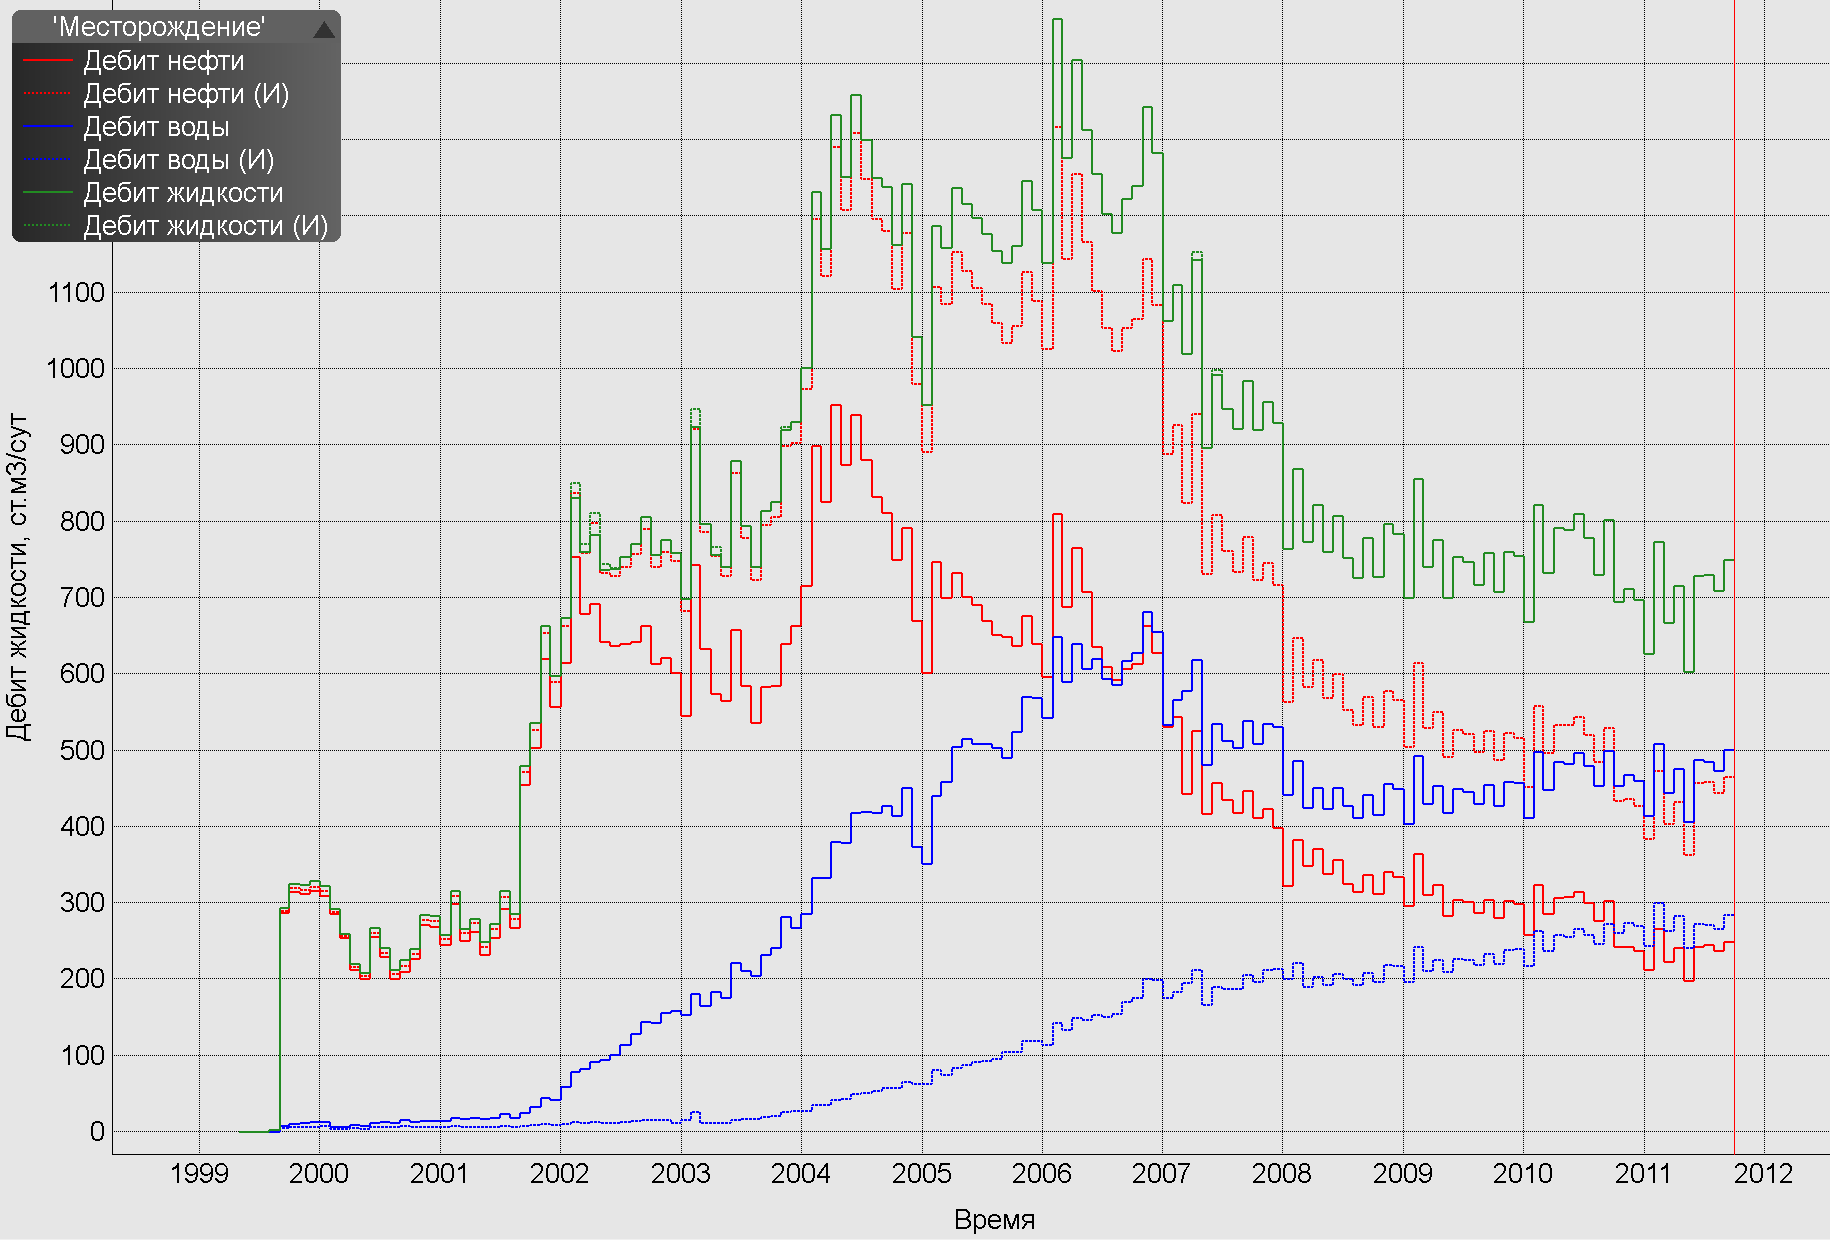
\includegraphics[width=\textwidth]{model_not_adapt}
\caption{Рассчитанные и исторические графики дебитов нефти, воды и жидкости (суммарно со всех скважин по месторождению) для исходной модели}
\label{fig:history_before_adaptation}
\end{figure}

Из рис. \ref{fig:history_before_adaptation} видим, что рассчитанные и исторические значения дебитов жидкости практически совпадают, а рассчитанные и исторические значения дебитов нефти/воды сильно отличаются друг от друга.
Дополнительно проверены зависимости дебитов для каждой из скважин в модели -- ситуация аналогична, т.е. по жидкости история и расчёт практически совпадают, а по дебитам воды/нефти есть большие невязки расчёта с историей работы скважин. 

Далее будем проводить адаптацию модели с целью минимизации невязок рассчитанных и исторических дебитов воды/нефти.

При адаптации модели для достижения поставленной цели варьируются параметры модели (исходные данные), обладающие неопределённостью.



\newpage
\section{Задание от 09.11.2022}

Решить уравнение фильтрации однофазной жидкости в одномерном пласте, используя явную схему метода конечных разностей.

Jupyter-тетрадь с решением доступна по ссылке: \href{https://colab.research.google.com/github/mualal/notebooks-source/blob/master/10_one_dimensional_filtration.ipynb}{OPEN IN COLAB}

\newpage
\section{Задание от 16.11.2022}

Решить уравнение фильтрации однофазной жидкости в одномерном пласте, используя неявную схему метода конечных разностей.

Jupyter-тетрадь с решением доступна по ссылке: \href{https://colab.research.google.com/github/mualal/notebooks-source/blob/master/10_one_dimensional_filtration.ipynb}{OPEN IN COLAB}

\newpage
\section{Задание от 16.11.2022 (бонус)}

Решить уравнение фильтрации однофазной жидкости в двумерном пласте, используя неявную схему метода конечных разностей.

Jupyter-тетрадь с решением доступна по ссылке: \href{https://colab.research.google.com/github/mualal/notebooks-source/blob/master/12_two_dimensional_filtration.ipynb}{OPEN IN COLAB}

Дополнительно код протестирован с большим числом ячеек и количеством скважин: \href{https://colab.research.google.com/github/mualal/notebooks-source/blob/master/13_two_dimensional_filtration.ipynb}{OPEN IN COLAB}

\end{document}
